% =============================================================================
% Indirect reciprocity with asymmetric reputational inertia
% Integrated manuscript draft (main text, Methods, Extended Data and
% Supplementary Information). Revision 3, 14 November 2026.
%
% This file supersedes Manuscript_full_20261103.tex. Changes in revision 3
% are listed in REVISION_NOTES_20261114.md:
%   - new title, abstract and Introduction (framing "How should reputations
%     change?", built on the two steps of reputation formation);
%   - Results revised throughout; the former Extended Data Fig. 4 (ALLD--DISC
%     edge) and the explanation of basin changes are removed;
%   - Discussion extended by a section on reputation filters;
%   - displayed equations carry one relation per line;
%   - Supplementary Information reorganized into nine notes.
%
% Figures are searched in figures/ (Overleaf package) and in ../ (repository).
% Extended Data figure files are numbered as in this manuscript: ED_FigN.pdf
% is Extended Data Fig. N (N = 1-8). The files were renamed on 14 November
% 2026, after the former Extended Data Fig. 4 (ALLD--DISC edge) was removed.
%
% Build:  pdflatex -> bibtex <jobname> -> bibtex SI -> pdflatex -> pdflatex
%         (latexmk -pdf also works). The second bibtex run builds the
%         separate Supplementary reference list (multibib).
%
% Draft notes are printed in dark red. Set \draftnotesfalse to hide them.
% =============================================================================
% Displayed equations are centred. Add the class option fleqn to set them
% flush left, as in the wlscirep template.
\documentclass[10pt]{wlscirep}
\usepackage[T1]{fontenc}
\usepackage{amsthm,bm,mathrsfs,array,longtable}
\usepackage{placeins}
\usepackage[resetlabels]{multibib}
\newcites{SI}{Supplementary References}

\graphicspath{{figures/}{../}}
% Journal names are already abbreviated (Nature style) in references.bib.
\renewcommand{\JournalTitle}[1]{#1}
\setlength{\emergencystretch}{2em}
\allowdisplaybreaks
\def\UrlBreaks{\do\/\do\_\do-}
\captionsetup{font=small}

% Float placement: let figures share pages with text instead of forming
% separate float pages.
\renewcommand{\topfraction}{0.9}
\renewcommand{\bottomfraction}{0.6}
\renewcommand{\textfraction}{0.08}
\renewcommand{\floatpagefraction}{0.85}
\setcounter{topnumber}{2}
\setcounter{bottomnumber}{1}
\setcounter{totalnumber}{3}
\setlength{\textfloatsep}{14pt plus 3pt minus 3pt}

% ---------------------------------------------------------------- draft notes
\newif\ifdraftnotes
\draftnotestrue
\DeclareRobustCommand{\draftnote}[1]{%
  \ifdraftnotes{\color{red!60!black}\sffamily\footnotesize[#1]}\fi}

% ------------------------------------------------------------------- notation
\newcommand{\Rmap}{\mathscr{R}}            % reputation map
\newcommand{\Lspace}{\mathscr{L}}          % latent state space
\newcommand{\st}[1]{\mathrm{#1}}           % latent states G, B, W_m, S_n
\newcommand{\Pp}[1]{P^{+}_{\mathrm{#1}}}   % e.g. \Pp{C|G}
\newcommand{\rR}{r_{\mathrm{R}}^{*}}
\newcommand{\uR}{u_{\mathrm{R}}^{*}}
\newcommand{\rX}{r_{\mathrm{X}}^{*}}
\newcommand{\uX}{u_{\mathrm{X}}}
\newcommand{\PhiC}{\Phi_{\mathrm{C}}}
\newcommand{\PhiD}{\Phi_{\mathrm{D}}}
\newcommand{\PhiCs}{\Phi^{*}_{\mathrm{C}}}
\newcommand{\PhiDs}{\Phi^{*}_{\mathrm{D}}}
\newcommand{\dPhi}{\Delta\Phi^{*}}
\newcommand{\Hmin}{H_{\min}}
\newcommand{\Pone}{P_{1}}                  % price of one negative assessment
\newcommand{\dd}{\mathrm{d}}
\newcommand{\ALLC}{\mathrm{ALLC}}
\newcommand{\ALLD}{\mathrm{ALLD}}
\newcommand{\DISC}{\mathrm{DISC}}

% ------------------------------------------- statements (used in the SI only)
\theoremstyle{plain}
\newtheorem{lemma}{Lemma}
\newtheorem{proposition}[lemma]{Proposition}
\newtheorem{corollary}[lemma]{Corollary}
\theoremstyle{remark}
\newtheorem{remark}[lemma]{Remark}
\renewcommand{\thelemma}{S\arabic{lemma}}

% -------------------------------------------------------------------- figures
\newcommand{\figfile}[2][0.66]{%
  \includegraphics[width=\linewidth,height=#1\textheight,keepaspectratio]{#2}}

% ---------------------------------------------------------------- front matter
\title{Indirect reciprocity with asymmetric reputational inertia}

% Affiliations are numbered in order of first appearance. The asterisk marks
% the corresponding authors.
\author[1,2]{Wenqiang Zhu}
\author[1,2,3,4,*]{Xin Wang}
\author[1,2]{Xingru Chen}
\author[2,5]{Ming Wei}
\author[1,6,7,8,*]{Shaoting Tang}
\author[9]{Christian Hilbe}

\affil[1]{School of Artificial Intelligence, Beihang University, Beijing 100191, China}
\affil[2]{Key Laboratory of Mathematics, Informatics and Behavioral Semantics, Beihang University, Beijing 100191, China}
\affil[3]{Zhongguancun Laboratory, Beijing 100094, China}
\affil[4]{Beijing Advanced Innovation Center for Future Blockchain and Privacy Computing, Beihang University, Beijing 100191, China}
\affil[5]{School of Mathematics, Beihang University, Beijing 100191, China}
\affil[6]{Hangzhou International Innovation Institute, Beihang University, Hangzhou 311115, China}
\affil[7]{Institute of Trustworthy Artificial Intelligence, Zhejiang Normal University, Hangzhou 310012, China}
\affil[8]{Shandong Key Lab of Complex Medical Intelligence and Aging, Shandong Medical and Pharmaceutical University, Yantai 264003, China}
\affil[9]{Interdisciplinary Transformation University, Linz 4040, Austria}
\affil[*]{Corresponding authors, Xin Wang (wangxin\_1993@buaa.edu.cn) and Shaoting Tang (tangshaoting@buaa.edu.cn)}

% Abstract revised 26 November 2026, 150 words, unreferenced (Nature Human
% Behaviour allows up to 150).
\begin{abstract}
Reputations sustain cooperation through indirect reciprocity, and theory has asked how to define goodness. Yet in standard models one assessment can overturn a reputation, so that misjudgments under private assessment spread and undermine cooperation. Here we ask how reputations should change in response to new assessments. In our model, a reputation changes only after a run of contrary assessments, and losing good standing can require a longer or shorter run than regaining it. We find that where this inertia is placed matters more than how much there is. Inertia that protects the standing overturned by a norm's misjudgments makes private reputations accurate and consistent without communication, and cooperation stable and reachable from 70--88\% of initial conditions. Placed the other way, the same inertia can destroy cooperation. Tolerance also shelters opportunists, who are excluded once a single negative assessment lowers a reputation without reversing it, making it costly but not catastrophic.
\end{abstract}

\begin{document}
\raggedbottom
\maketitle

% =============================================================================
\section*{Introduction}
% Revision 10 (26 November 2026). Five paragraphs in an academic register:
% (1) reputation and cooperation, and the two processes of reputation formation
% (assessment and updating); (2) assessment, the classic question of how
% goodness should be defined, and the failure of agreement under private
% assessment; (3) updating, replacement in standard models, inertia in real
% reputations and in earlier models; (4) the direction of inertia, the two
% kinds of misjudgment and the research question; (5) "Here, we ...", the
% findings without numbers, and their significance. Framing B (agreement
% without communication) stays in the Discussion.

Reputations sustain cooperation among individuals who may never interact again~\cite{alexander1987,nowak1998,nowak2005}. Under indirect reciprocity, individuals who help others acquire a good reputation and are more likely to receive help from third parties~\cite{wedekind2000,milinski2002}, and people cooperate more when their actions are observable~\cite{yoeli2013}. A good reputation thereby substitutes for a shared history of interactions and extends cooperation beyond pairs of individuals who meet repeatedly~\cite{kandori1992,milinski2016,okada2020}. The formation of a reputation comprises two distinct processes. An observer first assesses an action according to a social norm and then updates its view of the actor in light of this assessment. Together, the two processes determine whether reputations reflect behavior and whether different observers agree about them, the two conditions on which reputation-based cooperation depends~\cite{michelmata2024}.

Whether an action merits a good reputation depends on the norm that observers apply~\cite{brandt2004,ohtsuki2004}, and refusing to help an individual in bad standing, for example, can be a justified sanction, not a defection~\cite{sugden1986,leimar2001,panchanathan2003}. Theory has accordingly asked how goodness should be defined~\cite{ohtsuki2004}, that is, which actions, in which contexts, deserve a good reputation~\cite{santos2018,kessinger2023,murase2024computational}. Its best-known answer, the leading-eight norms, sustains cooperation in the presence of errors, provided that reputations are public and all observers share the same view of everyone else~\cite{ohtsuki2004,ohtsuki2006}. Under private assessment, observers witness different interactions and perceive them imperfectly, so that their views of the same individual diverge~\cite{takahashi2006,uchida2010,uchida2013,hilbe2018}. Assessment then propagates these disagreements, since each observer evaluates an action in light of its own view of the recipient~\cite{hilbe2018,radzvilavicius2019,fujimoto2022}. Even rare errors can thereby erode the agreement on which reputation-based cooperation relies~\cite{murase2024synchronization}, and most leading-eight norms lose their stability~\cite{hilbe2018,okada2018,perret2021,fujimoto2023}. Proposed mechanisms restore agreement through public institutions, gossip and the synchronization of opinions~\cite{radzvilavicius2021,kawakatsu2024,murase2024synchronization,tham2026}, or make assessment more lenient through empathy, generosity and tolerance~\cite{radzvilavicius2019,schmid2021nhb,schmid2021,okada2017,okada2024}. These mechanisms act on the information that enters assessment or on the norm itself, and they leave the updating of reputations unchanged.

In standard models, updating takes its simplest form, in which the most recent assessment replaces the observer's previous view~\cite{ohtsuki2004,hilbe2018}. A single assessment, whether correct or erroneous, can then overturn a reputation established over many interactions, and under private assessment each misjudgment immediately alters the reputations against which subsequent actions are assessed. Reputations in human societies display inertia instead, as people revise their impressions of others incrementally~\cite{mendesiedlecki2013neural,siegel2018,yamamoto2025}, online platforms aggregate many ratings~\cite{tadelis2016}, and communities that manage common resources escalate sanctions only for repeated violations~\cite{ostrom1990,cox2010}. Models in which reputations accumulate evidence, in the form of quantitative scores~\cite{schmid2023}, records of past defections~\cite{clark2020} or samples of several observations~\cite{michelmata2024}, can sustain cooperation where models based on replacement predict its collapse. Related models allow intermediate reputations~\cite{tanabe2013,murase2022,lee2021}, stochastic or gradual updating~\cite{murase2023,yamamoto2025}, or no update when the recipient is in bad standing~\cite{sasaki2017,okada2018}. Cooperation therefore depends not only on how actions are assessed but also on how reputations change in response to new assessments.

Inertia can, moreover, differ between the two directions in which a reputation changes. Human judgments display asymmetries in both directions, in that trust is lost more easily than it is gained~\cite{slovic1993}, whereas beliefs about individuals who have behaved badly are revised more readily than beliefs about individuals who have behaved well~\cite{siegel2018}. In indirect reciprocity, the direction of inertia matters, as private assessment produces two kinds of misjudgment. Cooperators are wrongly condemned, as when an observer who disagrees with the donor about the recipient condemns a justified refusal to help~\cite{okada2020dilemmas}. Defectors are wrongly excused, as when a norm that approves of refusing help to individuals in bad standing allows an unconditional defector to pass as a justified punisher. Inertia that delays the loss of good standing absorbs wrongful condemnations but also shields excused defectors, whereas inertia that delays recovery absorbs wrongful excuses but also entrenches wrongful condemnations. Norms differ in the misjudgments they produce, and the direction of inertia that sustains cooperation may therefore differ between norms. These considerations raise the question of how reputations should change in response to new assessments, and whether the answer depends on the norm by which actions are judged.

Here, we address this question using a model of indirect reciprocity with asymmetric reputational inertia (Fig.~\ref{fig:model}). An established reputation changes only after a run of contrary assessments, the run required to lose good standing can differ from the run required to regain it, and incomplete evidence can already have partial consequences. We find that the placement of inertia matters more than its amount. Inertia sustains cooperation when it protects the standing that a norm's misjudgments overturn, namely good standing under Scoring and Shunning, bad standing under Simple Standing and both under Stern Judging. A small number of intermediate states placed in this way allows observers to distinguish cooperators from defectors and to agree about reputations, renders cooperation evolutionarily stable and enlarges its basin of attraction, including under Shunning and Stern Judging, which fail without inertia. The same inertia placed in the opposite direction can eliminate cooperation. Tolerance of isolated negative assessments, however, also shelters opportunists who withhold help in a fraction of their interactions, and they are excluded only when a single negative assessment is costly but not catastrophic, lowering a reputation without reversing it. Our results identify the updating of reputations as a determinant of cooperation distinct from the definition of goodness. They suggest that norms and the rules by which reputations change should be studied together, and that the stability of reputation systems, from informal communities to formal institutions, depends on how they weigh new evidence against established standing.

% =============================================================================
\section*{Results}

\subsection*{A model of asymmetric reputational inertia}

We study a well-mixed population in which randomly matched donors and recipients play the donation game, in which helping costs the donor $c$ and gives the recipient a benefit $b>c$ (Methods). Unconditional cooperators (ALLC) intend to help every recipient, unconditional defectors (ALLD) intend to help no one, and discriminators (DISC) help only recipients they regard as good. Reputations are private~\cite{hilbe2018,okada2018}, in the sense that each observer keeps its own record of every other individual and judges a donor's action by its own view of the recipient. We compare four second-order norms, Scoring (SC), Shunning (SH), Stern Judging (SJ) and Simple Standing (SS)~\cite{ohtsuki2004,pacheco2006}, which judge actions towards a recipient in good standing in the same way and differ in how they judge actions towards a recipient regarded as bad. Intended help fails with probability $e_1$, and assessments are reversed with probability $e_2$ (Methods).

Under instantaneous updating, as in the classic models, each new assessment replaces the observer's previous image of the donor (Fig.~\ref{fig:model}a). Under inertial updating, an established reputation changes only after a run of contrary assessments (Fig.~\ref{fig:model}b). An individual in good standing passes through $k_1$ warning states before it loses this standing, and an individual in bad standing passes through $k_2$ recovery states before it regains good standing. Losing good standing thus takes $k_1+1$ consecutive negative assessments, and regaining it takes $k_2+1$ consecutive positive ones. We call $k_1$ the tolerance depth, $k_2$ the strictness depth and $K=k_1+k_2$ the total depth. Inertia is asymmetric whenever $k_1\neq k_2$, and $(k_1,k_2)=(0,0)$ recovers instantaneous updating. The intermediate states can already have partial consequences, because a warning state is still treated as good with a probability set by the tolerance strength $\alpha$, and a recovery state is still treated as bad with a probability set by the strictness strength $\beta$ (Methods).

\begin{figure}[!t]
\centering
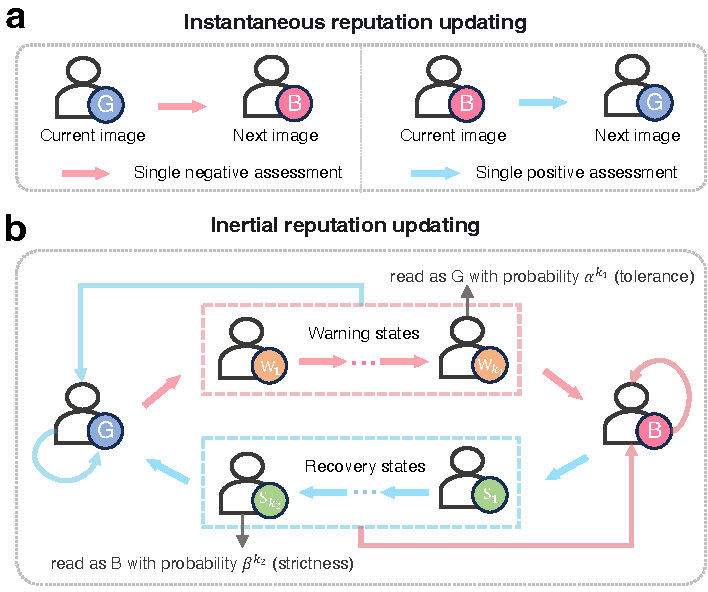
\includegraphics[width=0.6\linewidth]{Fig1_model}
\caption{\textbf{Instantaneous and inertial updating of reputations.}
Each observer keeps a private record of every other individual, and each assessment that the observer makes of a donor updates its record of that donor. Pink and blue arrows denote negative and positive assessments throughout the figure.
\textbf{a}, Under instantaneous updating, the record holds only a good (G) or a bad (B) image, and every assessment replaces it, so that a single negative assessment turns G into B and a single positive one turns B into G.
\textbf{b}, Under inertial updating, consecutive negative assessments move a record in good standing through $k_1$ warning states $\st W_1,\ldots,\st W_{k_1}$ (orange) to B, and consecutive positive assessments move a record in bad standing through $k_2$ recovery states $\st S_1,\ldots,\st S_{k_2}$ (green) to G. An assessment that supports the established standing returns the record directly to G or B, and it leaves an established record unchanged (loops). The tolerance depth $k_1$ and the strictness depth $k_2$ are set independently, so that losing good standing takes $k_1+1$ consecutive negative assessments and regaining it takes $k_2+1$ consecutive positive ones. When the record is consulted, warning state $\st W_m$ is read as good with probability $\alpha^m$ (tolerance strength $\alpha$), and recovery state $\st S_n$ is read as bad with probability $\beta^n$ (strictness strength $\beta$). The diagram gives these probabilities for the last state of each path. With $\alpha=\beta=1$, an established image persists until a path is completed, and with smaller strengths, incomplete evidence already has partial consequences.}
\label{fig:model}
\end{figure}

In the population-level theory, every rule that turns assessments into reputations acts through a single function, the reputation map $\Rmap(u)$. It gives the stationary probability that an individual is regarded as good when the assessments it receives are positive with probability $u$ (Methods). Without inertia, $\Rmap(u)=u$, and every negative assessment counts in full. With full strengths, warning states flatten the map near $u=1$ and thereby make the reputation of an individual in good standing insensitive to isolated negative assessments, and recovery states flatten it near $u=0$, with the mirror effect on individuals in bad standing. Throughout, we compare instantaneous updating, symmetric one-step inertia ($k_1=k_2=1$ with $\alpha=\beta=1$) and norm-specific asymmetric architectures with $\alpha=\beta=1$, which we identify next.

% -----------------------------------------------------------------------------
\subsection*{Asymmetric inertia makes private reputations accurate and consistent}

To support cooperation, reputations need to distinguish cooperative from defective strategies, and different observers need to share them. We measured both properties in simulated finite populations with equal numbers of ALLC, ALLD and DISC individuals, in which every DISC observer keeps a separate record of every individual and strategies do not change (Methods). We measure accuracy by the reputational separation $\Delta g$, the difference between the probability that the cooperative strategies are regarded as good and the probability that ALLD is, and consistency by the mean disagreement $\bar d$, the probability that two DISC observers hold different images of the same individual (Methods).

Without inertia, each norm fails in its own way (Fig.~\ref{fig:recognition}a--d, top row). Under SC, which condemns every refusal to help, two observers disagree about a discriminator with probability 0.50. Under SH, which condemns every action towards a recipient regarded as bad, fewer than 5\% of images are good. Under SJ, where every assessment depends on the observer's view of the recipient, two observers disagree about any individual with probability 0.50, and under SS, which approves of refusing help to recipients regarded as bad, observers regard ALLD as good with probability 0.30. Under all four norms, private assessment wrongly condemns cooperators, and under SS and SJ it also wrongly excuses defectors, whose refusals are approved whenever the observer regards the recipient as bad (Supplementary Note~\ref{si:interactions}). Symmetric one-step inertia does not repair these failures (Fig.~\ref{fig:recognition}a--d, middle row). Under SH, for example, observers now agree, but only that everyone is bad, with fewer than 0.2\% of images good, which shows that agreement alone does not suffice.

\begin{figure}[!t]
\centering
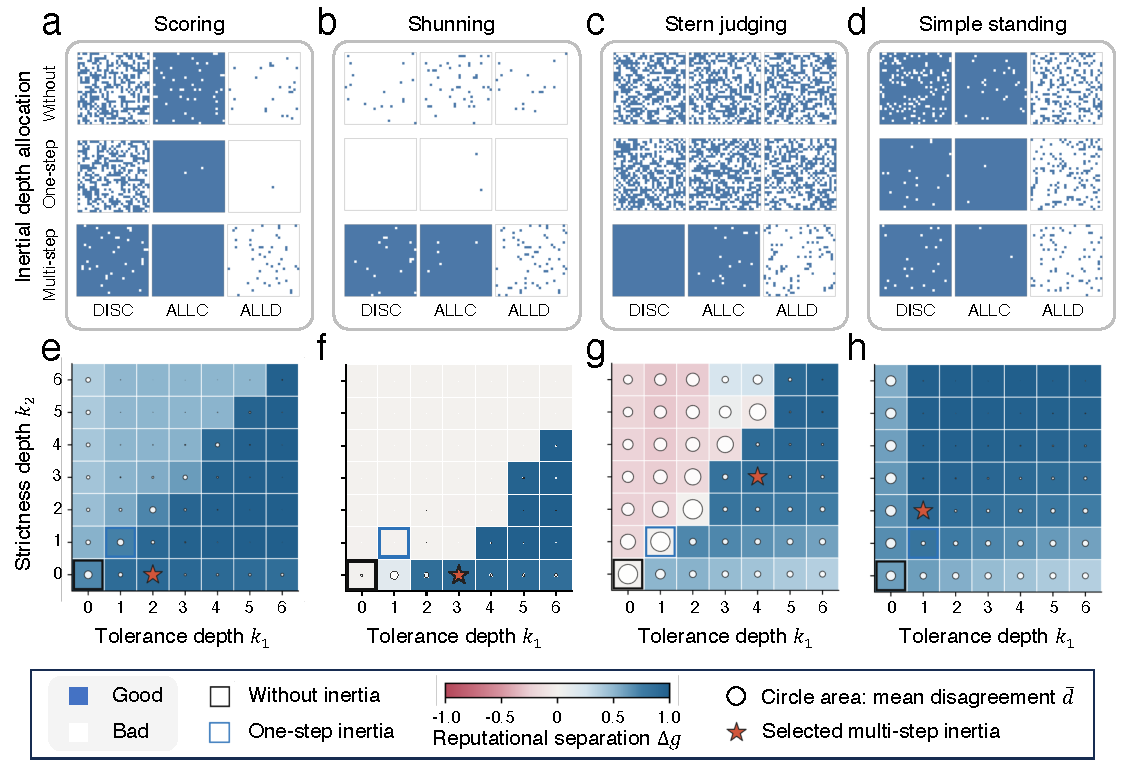
\includegraphics[width=0.9\linewidth]{Fig2}
\caption{\textbf{Accuracy and consistency of private reputations across inertial architectures.}
\textbf{a--d}, Private reputation matrices at the end of single simulation runs under Scoring (SC, \textbf{a}), Shunning (SH, \textbf{b}), Stern Judging (SJ, \textbf{c}) and Simple Standing (SS, \textbf{d}), without inertia, with full one-step inertia and with the selected architectures (rows of each panel). In each matrix, rows are the 30 DISC observers and columns are the 30 targets of each strategy, with blue and white cells showing good and bad images.
\textbf{e--h}, Reputational separation $\Delta g$ (color, Eq.~\eqref{eq:separation}) and mean disagreement $\bar d$ between DISC observers (circle area) for every depth pair with $0\leq k_1,k_2\leq6$, from single runs averaged over sweeps 800--1,000. Negative separations (red) mean that ALLD is regarded as good with a higher probability than the cooperative strategies. Black and blue outlines mark instantaneous updating, $(0,0)$, and one-step inertia, $(1,1)$. Stars mark the qualifying pair with the smallest total depth $K=k_1+k_2$ under the criteria $\Delta g\geq0.8$ and $\bar d\leq0.1$ (Methods), and replicated runs confirm this selection (Extended Data Fig.~\ref{ed:selection}).
Parameter values are equal numbers of the three strategies, $N=90$ in \textbf{a--d} and $N=150$ in \textbf{e--h}, 1,000 sweeps, $e_1=e_2=0.02$, and $\alpha=\beta=1$ for one-step and multi-step inertia.}
\label{fig:recognition}
\end{figure}

Both requirements are met when inertia is placed in a norm-specific direction (Fig.~\ref{fig:recognition}e--h). Using $\Delta g\geq0.8$ and $\bar d\leq0.1$ as operational criteria, we selected for each norm the qualifying allocation with the smallest total depth, which yields $(k_1,k_2)=(2,0)$ for SC, $(3,0)$ for SH, $(4,3)$ for SJ and $(1,2)$ for SS. All four architectures are asymmetric, and each asymmetry matches the misjudgments of its norm. Inertia protects good standing under SC and SH, where cooperators are wrongly condemned, it combines a single warning state with two recovery states under SS, where defectors are wrongly excused, and it acts on both paths under SJ. With these architectures, observers regard DISC and ALLC as good and ALLD as bad, with separations of 0.88--0.92 and disagreements of 0.06--0.08 (Fig.~\ref{fig:recognition}a--d, bottom row, and Extended Data Fig.~\ref{ed:selection}). Placing inertia in the other direction fails, as under SS, where warning states alone lower the separation from 0.61 to 0.43 as their number grows from zero to four, because tolerance then also protects defectors whose good standing stems from excuses (Fig.~\ref{fig:recognition}h). Replicated simulations confirm the selection, and the direction of each asymmetry persists over a range of criteria around the default (Extended Data Fig.~\ref{ed:selection} and Supplementary Table~\ref{tab:si-selected}). The selection uses reputation statistics only, without reference to evolutionary outcomes.

Inertia also changes the reputation dynamics of a population of discriminators (Extended Data Fig.~\ref{ed:resident}a--d). With one-step inertia, homogeneous DISC populations under SC, SH and SJ are bistable, so that the population's reputation depends on its history. In one stable state, residents are regarded as good with probability above 0.99, and in the other with probability below 0.001 under SC and SH and exactly 0.5 under SJ. The selected architectures remove this bistability and leave a single high-reputation state. Whether such a state exists, and whether it is unique, depends jointly on the two depths and the two strengths (Extended Data Fig.~\ref{ed:reputation-planes}). Asymmetric inertia thus makes private reputations both accurate and consistent, and we next ask whether such reputations allow cooperation to evolve.

% -----------------------------------------------------------------------------
\subsection*{Asymmetric inertia makes cooperation stable and enlarges its basin of attraction}

We let ALLC, ALLD and DISC evolve under the replicator dynamics~\cite{hofbauer1998}, assuming that reputations equilibrate faster than strategy frequencies change (Methods). At each strategy composition, payoffs are computed from the stationary private reputations reached from initially good records. To compare settings, we integrate the dynamics from 512 initial compositions and report the fraction of them that reach a cooperative state, which we call the cooperative basin, together with the mean realized cooperation $\bar\rho$.

Without inertia, a pure DISC population is not stable under any of the four norms (Fig.~\ref{fig:dynamics}a). SH and SJ sustain no cooperation at all, and under SC and SS cooperation persists only where discriminators are a minority, on a line of equilibria under SC and in a single mixture of ALLC and DISC under SS. This instability reflects the independence of private opinions when each interaction is assessed by a single observer~\cite{murase2024synchronization}. When every individual observes every interaction, Simple Standing can be stable without inertia~\cite{fujimoto2023}. Symmetric one-step inertia makes cooperative DISC populations locally stable under all four norms (Fig.~\ref{fig:dynamics}b), but the stable state is reached from only 8\% of initial compositions under SH and 23\% under SJ, and under SC the cooperative basin is no larger than without inertia.

\begin{figure}[!t]
\centering
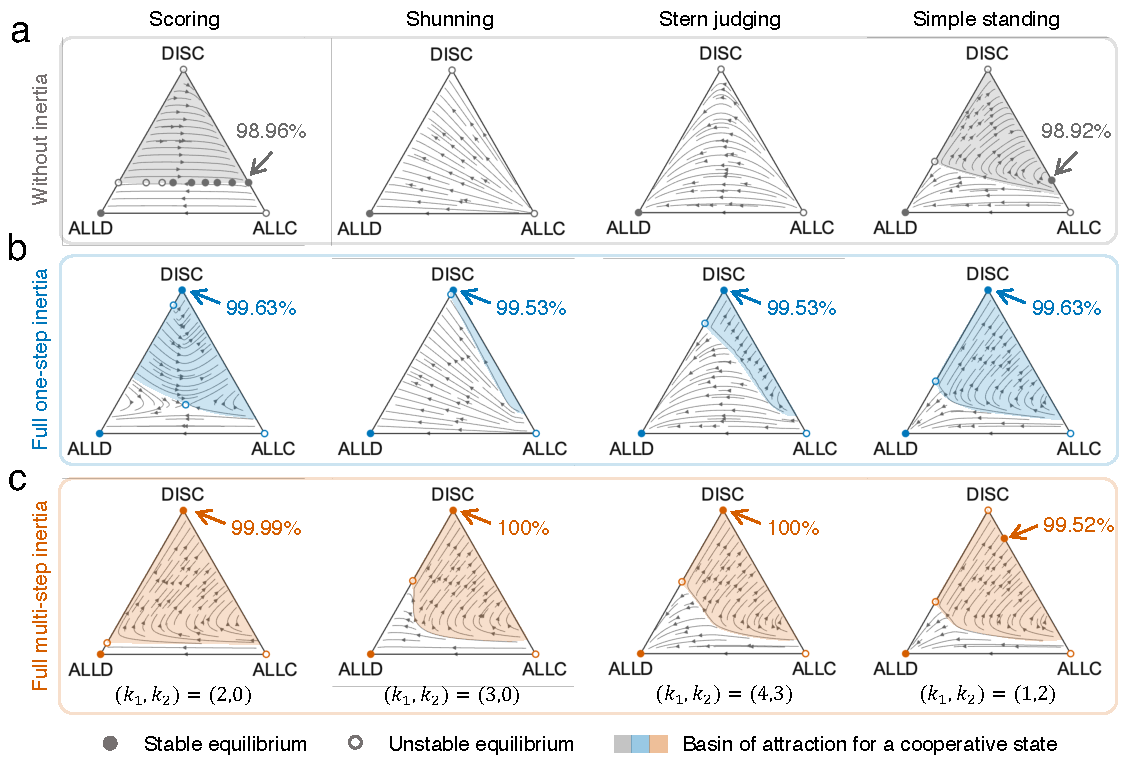
\includegraphics[width=0.9\linewidth]{Fig3}
\caption{\textbf{Evolution of cooperation without inertia, with one-step inertia and with the selected architectures.}
\textbf{a--c}, Evolutionary dynamics of ALLC, ALLD and DISC under SC, SH, SJ and SS (columns) without inertia (\textbf{a}), with full one-step inertia (\textbf{b}) and with the selected architectures (\textbf{c}, with depths $(k_1,k_2)$ given below each simplex). Vertices are pure populations, and streamlines show the replicator dynamics, with reputations at their stationary values, relaxed from initially good records, at every composition (Methods). Filled and open circles mark stable and unstable equilibria, and for equilibria on an edge they refer to stability along that edge. Shading marks the basin of attraction of a cooperative state, and percentages give intended cooperation at the stable cooperative equilibria. Without inertia, SC has a line of equilibria on which all three strategies obtain the same payoff, and filled and open circles along this line mark where it attracts and where it repels nearby populations (Supplementary Note~\ref{si:evolution}). Parameter values are $b/c=5$, $e_1=e_2=0.02$ and $\alpha=\beta=1$.}
\label{fig:dynamics}
\end{figure}

The selected architectures make cooperation stable and enlarge its basin of attraction (Fig.~\ref{fig:dynamics}c). Under SC, SH and SJ, pure DISC is a stable equilibrium at which discriminators intend to cooperate with probability above 0.9999. Under SS, unconditional cooperators can invade pure DISC, and the population settles in a stable mixture in which discriminators form the majority and intended cooperation exceeds 99\%. Under all four norms, the cooperative state is reached from 70--88\% of initial compositions. Averaged over the trajectories that reach a cooperative state, realized cooperation is 0.96--0.98 with or without inertia, so that mean cooperation follows the size of the cooperative basin (Supplementary Note~\ref{si:evolution} and Supplementary Table~\ref{tab:si-basins}).

Why stability requires inertia can be seen from the invasion of an established DISC population by rare unconditional mutants. Let $\rR$ denote the probability that a resident is regarded as good, and let $\PhiCs$ and $\PhiDs$ denote the probabilities that intended cooperation and intended defection towards a resident are assessed positively (Methods). Rare ALLC and ALLD mutants then have the reputations $\Rmap(\PhiCs)$ and $\Rmap(\PhiDs)$. When ALLD is regarded worse and ALLC better than the residents, pure DISC resists both mutants if and only if
\begin{equation}
R_{\mathrm L}\equiv\frac{\rR}{\rR-\Rmap(\PhiDs)}<\frac{b}{c}<\frac{1-\rR}{\Rmap(\PhiCs)-\rR}\equiv R_{\mathrm U}.
\label{eq:window}
\end{equation}
The lower bound $R_{\mathrm L}$ requires ALLD to lose more help than the cost it saves, and the upper bound $R_{\mathrm U}$ requires ALLC to gain less through its better reputation than it pays for also helping recipients regarded as bad.

The window has a geometric interpretation, because residents intend to help with probability $\rR$, so that the assessments they receive are a mixture of those received by ALLC and ALLD. The window is non-empty if and only if the reputation map lies above its chord between $\PhiDs$ and $\PhiCs$ (Methods). Without inertia, the map is linear and coincides with its chord, so that the two bounds coincide and no benefit-to-cost ratio protects discriminators against both mutants (Supplementary Note~\ref{si:unconditional}), whereas inertia bends the map and opens the window. With one-step inertia, the upper bound lies between 5.6 and 6.3, close to the reference ratio $b/c=5$, whereas the selected architectures raise it to about 230 under SC, 4,400 under SH and 21,000 under SJ (Supplementary Table~\ref{tab:si-thresholds}). Under SS, the upper bound of the selected architecture lies at $b/c\approx4$, below the reference ratio, which is why ALLC can invade pure DISC under SS and why the population settles in the mixture of Fig.~\ref{fig:dynamics}c instead of losing cooperation.

Beyond the reference conditions, the selected architectures reach similar cooperation from all-good and all-bad initial reputations, whereas one-step inertia under SH and SJ loses cooperation when records start bad (Extended Data Fig.~\ref{ed:resident}e--h). They support at least as much cooperation as instantaneous updating and one-step inertia at every sampled benefit-to-cost ratio from 1 to 10, and more at all but the lowest (Extended Data Fig.~\ref{ed:benefit-cost}). At one-step depths, tolerance alone makes pure DISC stable under every norm, with intended cooperation above 99.8\%, whereas strictness alone does not (Extended Data Fig.~\ref{ed:readout}). Under SH and SJ, the selected architectures also exclude ALLD in 69\% and 86\% of the plane of implementation and assessment errors up to 0.45, compared with about 1\% under one-step inertia (Extended Data Fig.~\ref{ed:errors}). They differ from one-step inertia both in where their intermediate states are placed and in how many there are, and we next separate these two factors.

% -----------------------------------------------------------------------------
\subsection*{Where inertia is placed matters more than how much there is}

Comparing all allocations $(k_1,k_2)$ with the same total depth $K$ shows that cooperation depends on which path receives the intermediate states (Fig.~\ref{fig:depth}). Under SC with two intermediate states, placing both on the recovery path leaves no cooperation, whereas placing both on the warning path yields $\bar\rho=0.87$. Across all depths, allocations that only slow recovery sustain no cooperation under SC, SH and SJ. Under these three norms, adding a recovery state to a single warning state, which yields symmetric one-step inertia, even lowers mean cooperation, so that more inertia can be worse than less. Under SS, by contrast, neither path alone raises mean cooperation by more than 0.02 above its value without inertia, 0.54, and longer paths of either kind lower it. Warning states alone lower cooperation as their number grows, in line with the protection they give to excused defectors. Cooperation increases only when a short warning path is combined with a longer recovery path.

\begin{figure}[!t]
\centering
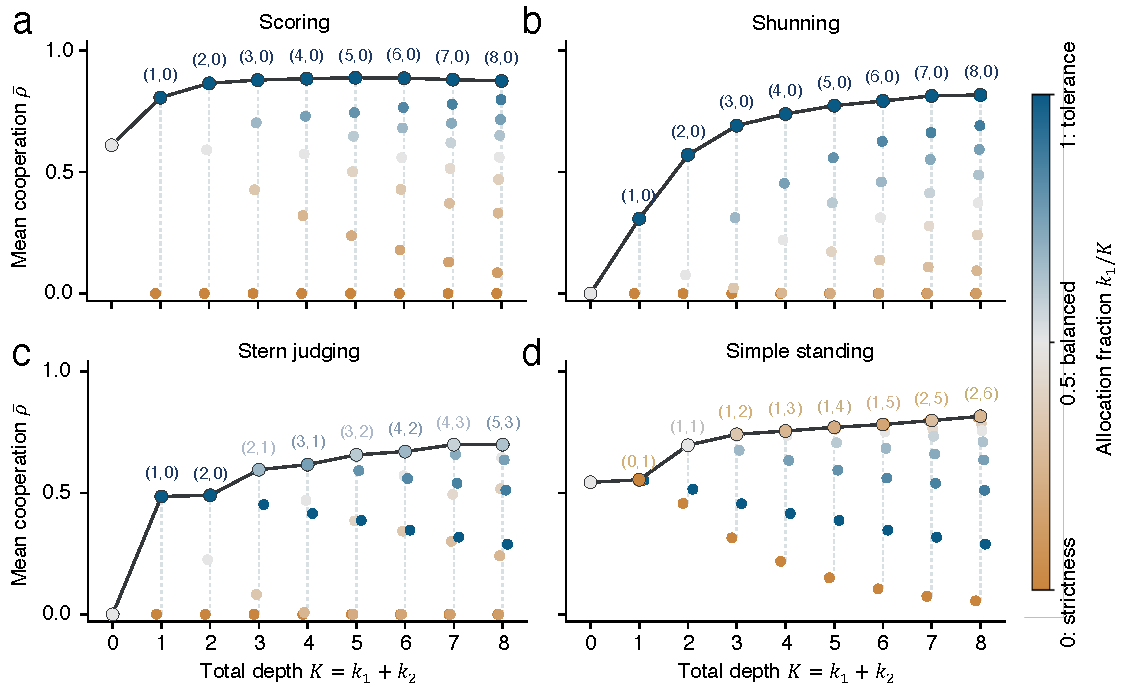
\includegraphics[width=0.85\linewidth]{Fig4}
\caption{\textbf{Mean cooperation for every allocation of a given total depth.}
\textbf{a--d}, Mean realized cooperation $\bar\rho$ over 512 initial strategy compositions against total depth $K=k_1+k_2$ ($0\leq K\leq8$) under SC (\textbf{a}), SH (\textbf{b}), SJ (\textbf{c}) and SS (\textbf{d}). Each point is one allocation $(k_1,k_2)$, and the point at $K=0$ is instantaneous updating. Points are colored by the allocation fraction $k_1/K$, from all intermediate states on the recovery path (0, brown) through a balanced allocation (0.5, gray) to all states on the warning path (1, blue). Large outlined points, connected by black lines and labeled with their depths, mark the most cooperative allocation at each $K$. At a given total depth, cooperation depends on the allocation, and under SC with $K=2$, for example, $\bar\rho=0.87$ for $(2,0)$ and $\bar\rho=0$ for $(0,2)$. Initial compositions are sampled uniformly from the simplex (Methods). Parameter values are $b/c=5$, $e_1=e_2=0.02$ and $\alpha=\beta=1$.}
\label{fig:depth}
\end{figure}

The most cooperative allocations follow the asymmetries identified above. They place all states on the warning path under SC and SH, combine a longer warning path with a shorter recovery path under SJ, and pair a short warning path with a longer recovery path under SS. The full plane of depths shows the same pattern (Extended Data Fig.~\ref{ed:depth-plane}). The four architectures selected from reputation statistics alone are the most cooperative allocations at their respective depths, so that the reputational criteria identify architectures that also maximize cooperation for their depth.

Additional depth beyond these architectures yields diminishing returns, and under SC the most cooperative allocation gains less than 0.03 in mean cooperation beyond two warning states and declines beyond five. One reason is that tolerance also protects defectors, because under SC and SH an unconditional defector receives a positive assessment only through an assessment error, and each additional warning state makes it more likely that such an error restores its good image. In a DISC population, the selected SC and SH architectures regard a rare defector as good with probability 0.06 and 0.08, respectively, compared with less than 0.001 under one-step inertia (Supplementary Table~\ref{tab:si-thresholds}). Two to seven intermediate states, placed on the appropriate path, therefore suffice. Protecting good standing, however, means tolerating isolated negative assessments, and we finally ask whether individuals who withhold help in a fraction of their interactions can exploit this tolerance.

% -----------------------------------------------------------------------------
\subsection*{Full tolerance shelters opportunists, and partial consequences exclude them}

Tolerance protects discriminators against erroneous negative assessments, but the same protection might shelter individuals who defect deliberately in a fraction of their interactions. We therefore consider a rare opportunistic discriminator (O-DISC), which behaves like DISC except that it withholds help from a recipient it regards as good with probability $\delta$, independently in each interaction. The endpoints $\delta=0$ and $\delta=1$ correspond to DISC and ALLD. Let $\rX(\delta)$ denote the stationary probability that the mutant is regarded as good. Its payoff advantage over residents, in units of the expected cost of an intended donation, is
\begin{equation}
\Lambda(\delta)=\delta\,\rR-\frac{b}{c}\bigl[\rR-\rX(\delta)\bigr].
\label{eq:lambda}
\end{equation}
The first term is the cost that the mutant saves, and the second is the benefit that it loses through a worse reputation. A positive $\Lambda$ permits invasion, and resistance to ALLD establishes only $\Lambda(1)<0$, leaving partial opportunism, $0<\delta<1$, untested.

All five mechanisms compared in Fig.~\ref{fig:opportunism}a exclude ALLD under SJ, but this does not exclude partial opportunism. Under the selected architecture with full tolerance strength, every O-DISC mutant with $0<\delta<0.365$ can invade, and one-step inertia admits invasion for $0<\delta<0.0084$. Two other rules that buffer isolated negative assessments show similar windows, up to $\delta=0.14$ for an aggregation rule that assigns a good image if at least one of two sampled assessments is positive~\cite{michelmata2024} and up to $\delta=0.38$ for a bounded quantitative score~\cite{schmid2023}. Because these rules were neither optimized nor matched in memory to the inertial record, the comparison illustrates a shared vulnerability rather than a ranking (Supplementary Note~\ref{si:filters}). The vulnerability is a property of the reputation map rather than of the mechanism that produces it, and the aggregation rule, for example, has exactly the map of an inertial record with a single warning state and full tolerance strength (Methods).

\begin{figure}[!t]
\centering
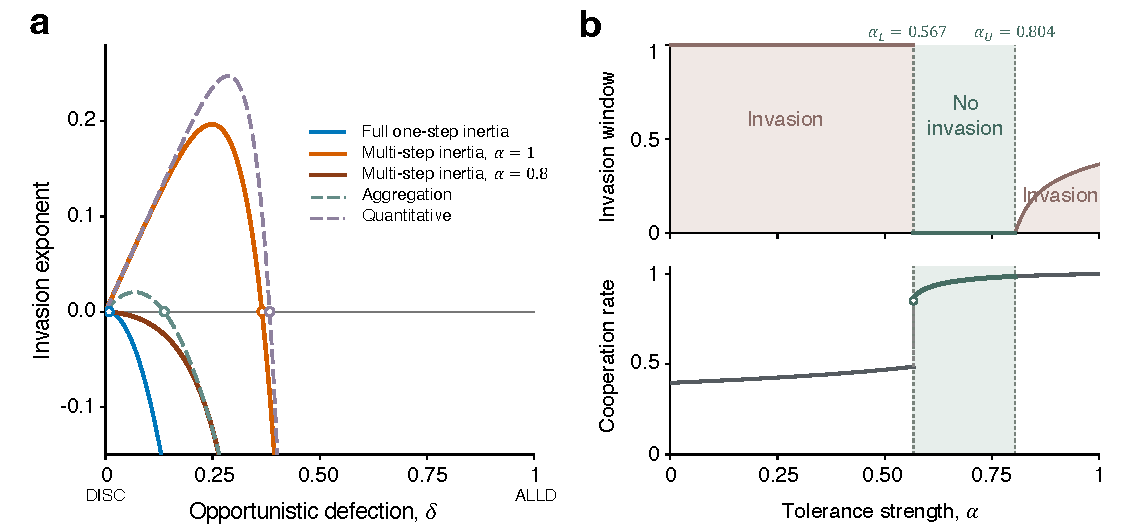
\includegraphics[width=0.9\linewidth]{Fig5}
\caption{\textbf{Invasion by opportunistic discriminators and the role of the tolerance strength.}
\textbf{a}, Payoff advantage $\Lambda$ (Eq.~\eqref{eq:lambda}) of a rare opportunistic discriminator (O-DISC) over a DISC resident under SJ, as a function of the probability $\delta$ with which it withholds help from recipients it regards as good (DISC at $\delta=0$ and ALLD at $\delta=1$). Curves compare full one-step inertia, the selected architecture $(4,3)$ with $\alpha=1$ and with $\alpha=0.8$, an aggregation rule that assigns a good image if at least one of two sampled assessments is positive\cite{michelmata2024}, and a bounded quantitative score\cite{schmid2023} (Methods). Positive values indicate invasion, and open circles mark where curves cross zero at $\delta>0$. All five mechanisms exclude ALLD, with $\Lambda(1)$ between $-4.0$ and $-3.8$, outside the plotted range (Supplementary Note~\ref{si:filters}).
\textbf{b}, Selected architecture $(4,3)$ as the tolerance strength $\alpha$ varies. The upper panel shows the upper end $\delta_c$ of the interval of omission probabilities that invade, and the lower panel shows the intended cooperation of residents, $\rR$. Below $\alpha_{\mathrm L}=0.567$, the high-reputation resident state no longer exists, residents cooperate with probability below 0.5, and every O-DISC mutant, including ALLD, invades ($\delta_c=1$), whereas above $\alpha_{\mathrm U}=0.804$ weak opportunists invade again. In the shaded secure range, $\alpha_{\mathrm L}<\alpha\leq\alpha_{\mathrm U}$, residents resist every O-DISC mutant and cooperate with probability above 0.85. Parameter values are $b/c=5$, $e_1=e_2=0.02$ and $\beta=1$.}
\label{fig:opportunism}
\end{figure}

This vulnerability originates in the reputational response to weak opportunism. At $\delta=0$, the slope of the invasion payoff is
\begin{equation}
\Lambda'(0)=\rR\Bigl[1-\frac{b}{c}\,\dPhi\,\Rmap'(\uR)\Bigr].
\label{eq:lambda-slope}
\end{equation}
The reputational cost of withholding help is thus a product of two factors, one for each of the two processes of reputation formation, assessment and updating. The assessment contrast $\dPhi$ measures how differently intended cooperation and intended defection towards a resident are judged, and the slope $\Rmap'(\uR)$ of the reputation map at the residents' positive-assessment probability $\uR$ measures how strongly a change in assessments moves a reputation (Methods). If the map is flat near the resident state, the benefit that weak opportunists lose through a worse reputation is smaller than the cost they save. Full tolerance strength produces this flatness, because for any architecture with a warning path, $\Rmap'(u)$ tends to $1-\alpha$ as $u$ tends to 1 (Supplementary Note~\ref{si:map}). Lowering $\alpha$ gives warning states an immediate chance of being read as bad and so restores a marginal penalty.

A negative slope at $\delta=0$ does not yet exclude larger omission probabilities. We therefore consider the reputation lost per unit of withheld cooperation, $H(\delta)=[\rR-\rX(\delta)]/(\delta\rR)$. Because $\Lambda(\delta)\leq0$ exactly when $H(\delta)\geq c/b$, the resident excludes the entire O-DISC family if and only if
\begin{equation}
\Hmin\equiv\min_{0\leq\delta\leq1}\frac{\rR-\rX(\delta)}{\delta\,\rR}\geq\frac{c}{b},
\label{eq:security}
\end{equation}
where the ratio at $\delta=0$ is defined by its limit, $\dPhi\,\Rmap'(\uR)$. Even the mutant with the smallest reputational penalty must gain nothing. In the error-free limit, the criterion takes a simple form. An all-good discriminator population with a warning path and full strictness strength then excludes every O-DISC mutant if and only if $\alpha\leq1-c/b$, under all four norms and for any strictness depth (Methods). The condition has a direct interpretation, because an isolated negative assessment leads to a bad image with probability $1-\alpha$, and the benefit expected to be lost in this way, $b(1-\alpha)$, must be at least as large as the cost $c$ that a defection saves.

Lowering the tolerance strength can therefore exclude opportunists while preserving cooperation. For the selected SJ architecture, reducing $\alpha$ from 1 to 0.8 excludes every O-DISC mutant, and residents still cooperate with probability 0.99 (Fig.~\ref{fig:opportunism}a). Below a critical value, however, lowering $\alpha$ destroys the high-reputation resident state, because a single negative assessment then leads to a bad image with probability $1-\alpha$, which approaches the value of 1 under instantaneous updating. Protection therefore holds within a bounded range, $\alpha_{\mathrm L}<\alpha\leq\alpha_{\mathrm U}$, which here extends from about 0.57 to 0.80 (Fig.~\ref{fig:opportunism}b). The lower boundary is a fold of the high-reputation state and does not depend on $b/c$. The upper boundary marks the point at which the weakest opportunists become neutral, and it rises with $b/c$ (Methods).

Protective tolerance strengths exist under all four norms, although their location depends on the norm and the architecture (Extended Data Fig.~\ref{ed:security}). At $\alpha=0.8$, all four selected architectures resist the O-DISC family, and residents are regarded as good with probability 0.98--0.99, whereas one-step inertia under SH and SJ has already lost its high-reputation state. Because the fold is fixed while the upper boundary rises with $b/c$, protective ranges shrink at low benefit-to-cost ratios and can vanish, as under SH at $b/c=2$.

These results concern omissions that occur independently in each interaction and do not cover persistent or temporally correlated opportunism. They also have a mirror image, because once withholding help costs more reputation than it saves, helping marginally more than residents do becomes worthwhile. At $\alpha=0.8$, the upper bound $R_{\mathrm U}$ of Eq.~\eqref{eq:window} accordingly lies below the reference ratio under all four norms, and ALLC can enter a pure DISC population. Under SC, SH and SJ, this invasion stops in a mixture with less than 3\% ALLC, in which intended cooperation is about 0.99 and the growth rate of rare ALLD is below $-3.4$ in units of $c$ (Supplementary Note~\ref{si:generous}).
\draftnote{The DISC--ALLC mixtures at $\alpha=0.8$ (Supplementary Table~\ref{tab:si-generous}) were reproduced on 25 November 2026 with an independent implementation of the mean-field equations. Add this calculation to the verified package before submission.}

Depth and strength therefore serve different functions in a reputation system. The depths, and their asymmetry, determine whether a single assessment can overturn a reputation, and thereby whether reputations are accurate and how large the basins of cooperative states are. The strength of warning states determines what a single negative assessment costs at the margin, and thereby whether tolerance can be exploited. A single negative assessment is thus catastrophic under instantaneous updating and costless under full tolerance, whereas with partial consequences it is costly but not catastrophic.

% =============================================================================
\section*{Discussion}
% Revised 25 November 2026. Seven paragraphs: the answer to the question posed
% in the Introduction; agreement without communication (framing B); norms and
% the rules for changing reputations; the price of tolerance and why
% consequences must be graded; human judgments and institutions; limitations;
% closing. The comparison of reputation filters and the open question of which
% filter is best are in Supplementary Note si:filters.

We asked how reputations should change in response to new assessments. Our results suggest that, when assessments are private, reputations should change slowly, asymmetrically and with graded consequences. Inertia sustains cooperation when it protects the standing that a norm's misjudgments overturn, and placed the other way it entrenches misjudgments instead of absorbing them. Two to seven intermediate states suffice, and more can reduce cooperation, because the tolerance that protects cooperators also protects defectors. This is in line with the finding that individuals who can choose how many observations to use evolve to use fewer than are available~\cite{michelmata2024}. While contrary evidence accumulates, it should already have partial consequences, so that a single negative assessment is costly but not catastrophic. None of these properties concerns which actions are judged good, because they concern how each new judgment is weighed against earlier ones.

Observers who update their records independently and never communicate can still arrive at shared and accurate views. Theory predicts that reputation-based cooperation can evolve only if individuals' opinions of one another are sufficiently correlated~\cite{murase2024synchronization,tham2026}. Our observers exchange no information, and our mean-field theory treats their opinions of an individual as independent once its strategy is given. With suitably placed inertia, they nevertheless agree, with disagreements of 0.06--0.08, and their shared view separates cooperators from defectors. Reliable private judgments coincide, because two observers who independently regard an individual as good with probability $r$ disagree with probability $2r(1-r)$, which approaches zero as $r$ approaches zero or one. Agreement alone, however, is not enough, because under Shunning with one-step inertia observers agreed that everyone was bad, with fewer than 0.2\% of images good. Accuracy thus implies agreement, but agreement does not imply accuracy. Nor does independence prevent stable cooperation once reputations have inertia. When each assessment replaces the previous view, independent opinions make one of the two unconditional strategies a best response to discriminators~\cite{murase2024synchronization}, but inertia bends the reputation map and allows discriminators to resist both. Inertia can be combined with mechanisms that align opinions, such as institutions, gossip and synchronization~\cite{radzvilavicius2021,kawakatsu2024,murase2024synchronization}, but unlike them it needs no communication, whose requirements include, for gossip, a minimum amount of exchange~\cite{kawakatsu2024}.

How reputations change also affects which norms succeed, as the example of Stern Judging shows. Stern Judging is among the most successful norms when reputations are public~\cite{santos2018}, but under private assessment it fails to distinguish friend from foe~\cite{hilbe2018} and cannot be evolutionarily stable, because errors accumulate~\cite{fujimoto2023}. With inertia on both paths, Stern Judging yielded accurate and consistent reputations, and cooperation was stable and reached from 71\% of initial conditions. Shunning, under which fewer than 5\% of images are good without inertia, sustained cooperation with warning states alone. Comparisons and evolutionary analyses of norms~\cite{kessinger2023,murase2024computational} may reach different conclusions once reputations have inertia, and norms and the rules for changing reputations may need to be studied together.

Tolerance can be exploited, because a rule for changing reputations sees only assessments and cannot tell a wrongful condemnation from a deserved one, so that any rule that forgives isolated negative assessments also forgives isolated defections. This tension between correcting errors and inviting exploitation, noted for generous assessment~\cite{schmid2021}, also affects inertial records and the forgiving forms of aggregation and quantitative scores. Discriminators that resisted unconditional defectors were invaded by opportunists, so that stability against unconditional strategies is not a sufficient test of a reputation system. The tension has a resolution that applies to any rule for changing reputations (Supplementary Note~\ref{si:filters}). The relevant quantity is the price of a negative assessment, the expected time for which one isolated negative assessment makes an observer regard an individual as bad, in units of the interval between that observer's assessments of the individual. In the error-free limit, deterring opportunists requires a price of at least $c/b$, whereas preventing misjudgments from spreading requires a price below one, or below one half under Shunning and Stern Judging. A rule that reads each of its states as definitely good or definitely bad charges a whole-number price and therefore fails one of the two requirements. Both can be met only with graded or probabilistic consequences, such as warning states that are read as bad with a probability between zero and one. This is the general content of the principle that a single negative assessment should be costly but not catastrophic.

Human impressions are revised asymmetrically, but not always in the same direction. Trust is fragile~\cite{slovic1993}, beliefs about bad people are volatile~\cite{siegel2018}, and the direction differs between judgments of morality and of ability~\cite{reeder1979,skowronski1989,mendesiedlecki2013diagnostic}. Our results suggest one reason, namely that the direction that favors cooperation depends on how a community judges refusals to help. Where refusing help to someone in bad standing is condemned, as under Scoring and Shunning, good standing should be hard to lose. Where such refusals are approved, as under Simple Standing, bad standing should be hard to shed. Experiments that vary the norm by which participants judge others could test whether the direction of their updating follows it. A second prediction concerns incomplete evidence, namely that an individual with a single recent lapse should be treated less favorably than one with a clean record but better than one in bad standing. Scenario experiments suggest that people's evaluations of a donor do move one step at a time, through a neutral level between good and bad~\cite{yamamoto2025}. Institutions also distinguish incomplete from complete evidence, as graduated sanctions answer first violations with mild responses that escalate with repetition~\cite{ostrom1990,cox2010} and a criminal record loses its predictive value only after years without further offenses~\cite{blumstein2009}.

Our theory has several limitations that point to future work. It uses a mean-field closure that treats different observers' records as conditionally independent, and it evaluates strategy evolution at stationary reputations. Finite-population simulations support the reputational results, but simulations in which strategies and records change together would test this separation of timescales. Each interaction was assessed by a single observer, whereas when every individual observes every interaction, opinions become correlated and some norms sustain cooperation without inertia~\cite{fujimoto2023,murase2024synchronization}, and how inertia acts in that setting remains open. All individuals shared one architecture, chosen by us rather than evolved, and memory was free. Letting depths and strengths evolve, together with norms and at a cost, would show which architectures arise without design, and whether observers who reason about the reliability of their own assessments~\cite{pandula2024,morsky2024} arrive at similar rules. Our invasion analysis covered unconditional strategies and omissions that occur independently in each interaction, and persistent or temporally correlated defection deserves separate analysis. Finally, in our theory a discriminator population cannot strictly resist deviations in both directions, because once withholding help costs more reputation than it saves, helping marginally more than residents do becomes worthwhile and unconditional cooperators can enter. This possibility reflects the independence of private opinions~\cite{murase2024synchronization}, and inertia does not remove it, although the resulting mixtures kept intended cooperation of at least 0.987.

In standard models of indirect reciprocity, a reputation is a verdict on the latest action. In real communities, it is closer to a summary of evidence. Our results suggest that how this summary is kept, and in particular how much evidence it takes to change one's mind about another person in each direction, can decide whether cooperation among private observers succeeds.

% =============================================================================
\section*{Methods}
\label{sec:methods}
% Revised 26 November 2026. Only the formulas needed to follow the analysis
% are displayed. Explicit assessment probabilities, the stationary
% distribution of a record, special cases of the reputation map, the
% population-level assessment probabilities, the boundaries of secure
% intervals, the simulation estimators and all numerical settings are given
% in the Supplementary Information. Equations displayed in the Results are
% cited rather than repeated.

\subsection*{Model}

We consider an infinitely large, well-mixed population in which randomly matched donors and recipients play the donation game. A donor either cooperates, paying a cost $c>0$ to give the recipient a benefit $b>c$, or defects, which has no payoff consequences. Individuals use one of three strategies $I\in\{\ALLC,\ALLD,\DISC\}$ with frequencies $f_I$. ALLC intends to cooperate with every recipient, ALLD intends to defect against every recipient, and DISC intends to cooperate if and only if it regards the recipient as good. All individuals share one social norm and one reputation mechanism, and strategy evolution changes only the frequencies $f_I$.

Reputations are private~\cite{okada2018,hilbe2018,radzvilavicius2019}, so that every individual keeps its own record of every other individual, and in each interaction an observer, drawn independently of the donor and the recipient, assesses the donor. A DISC donor acts on its own image of the recipient, whereas the observer judges the donor's action by its own image of the recipient, so the two can disagree. We use second-order norms~\cite{ohtsuki2004}, under which cooperation with a recipient regarded as good is assessed positively and defection against such a recipient negatively. Towards a recipient regarded as bad, cooperation and defection are assessed positively with probabilities $p$ and $q$, so that SC, SH, SJ and SS correspond to $(p,q)=(1,0)$, $(0,0)$, $(0,1)$ and $(1,1)$. Intended cooperation fails with probability $e_1$, intended defection is always implemented, and the observer records the opposite of the prescribed assessment with probability $e_2$. Unless stated otherwise, the parameter values are $b=5$, $c=1$ and $e_1=e_2=0.02$.

We write $\Pp{A|Y}$ for the probability that the recorded assessment is positive when the donor intends action $A\in\{\st C,\st D\}$ and the observer regards the recipient as $Y\in\{\st G,\st B\}$. These probabilities combine the norm with both kinds of error, and their explicit forms are given in Supplementary Note~\ref{si:interactions} and Supplementary Table~\ref{tab:si-norms}. If the observer regards the recipient as good with probability $r$, intended cooperation and intended defection are assessed positively with probabilities $\PhiC(r)$ and $\PhiD(r)$, the averages of $\Pp{C|Y}$ and $\Pp{D|Y}$ over the observer's image. Their difference, $\Delta\Phi(r)=\PhiC(r)-\PhiD(r)$, is the assessment contrast, which measures how much better intended cooperation is judged than intended defection.

\subsection*{Inertial records and the reputation map}

Observer $i$ holds a latent record $L_{ij}$ of target $j$, with the states $\st G,\st W_1,\ldots,\st W_{k_1},\st B,\st S_1,\ldots,\st S_{k_2}$. After an interaction, only the observer's record of the donor changes, and only through the recorded assessment (Fig.~\ref{fig:model}b). Negative assessments move a record from G through the warning states to B, and positive assessments move it from B through the recovery states to G. An assessment that supports the established judgment returns a warning state to G and a recovery state to B. Consecutive assessments are those made by the same observer about the same target (Supplementary Note~\ref{si:record} and Supplementary Table~\ref{tab:si-transitions}). Whenever a record in state $\ell$ is consulted, to act or to assess, it yields a good image with probability
\begin{equation}
\sigma(\ell)=
\begin{cases}
1, & \ell=\st G,\\
\alpha^m, & \ell=\st W_m,\\
0, & \ell=\st B,\\
1-\beta^n, & \ell=\st S_n,
\end{cases}
\label{eq:m-readout}
\end{equation}
independently of other consultations and without changing the state. Instantaneous updating corresponds to $(k_1,k_2)=(0,0)$, or equivalently to $\alpha=\beta=0$ at any depths (Supplementary Note~\ref{si:record}). At one-step depths, $(\alpha,\beta)=(1,0)$ and $(0,1)$ give tolerance only and strictness only.

If the successive assessments entering a record are independent and positive with probability $u$, the record follows a Markov chain on its $K+2$ states with a unique stationary distribution (Supplementary Note~\ref{si:map}). Averaging $\sigma$ over this distribution gives the reputation map, the stationary probability that the target is regarded as good. With $v=1-u$,
\begin{equation}
\Rmap(u)=\frac{u^{k_2+1}\sum_{m=0}^{k_1}(\alpha v)^m+v^{k_1+1}\sum_{n=1}^{k_2}u^n\bigl(1-\beta^n\bigr)}{v^{k_1}+u^{k_2}-v^{k_1}u^{k_2}},
\label{eq:m-map}
\end{equation}
with $\Rmap(0)=0$ and $\Rmap(1)=1$. Without inertia, $\Rmap(u)=u$, and with full strengths, $\Rmap(u)$ is the fraction of time that the record spends in good standing. An individual whose assessments are positive with a probability $u$ close to 1 is then regarded as bad with a probability of order $v^{k_1+1}$, and one with $u$ close to 0 is regarded as good with a probability of order $u^{k_2+1}$. For $k_1\geq1$, the slope of the map at $u=1$ is $\Rmap'(1)=1-\alpha$, where the prime denotes $\dd/\dd u$, and for $k_2=0$ the map is concave. These and further properties are derived in Supplementary Note~\ref{si:map}.

\subsection*{Private reputations in a population}

Let $r_I$ be the probability that a randomly chosen observer regards a randomly chosen type-$I$ individual as good, and $\bar r=\sum_If_Ir_I$. As in previous analyses of private assessment~\cite{okada2018,radzvilavicius2019,kessinger2023,michelmata2024,kawakatsu2024}, we close the model with two mean-field assumptions. First, the donor's and the observer's images of a recipient are independent given the recipient's strategy. Second, the assessments entering a record of a type-$I$ individual are independent, each positive with a common probability $u_I$. Under the first assumption, $u_I(\bm r;\bm f)$ follows from the probabilities $\Pp{A|Y}$ and the reputations. ALLC and ALLD donors are assessed positively with probabilities $\PhiC(\bar r)$ and $\PhiD(\bar r)$, whereas the assessment of a DISC donor depends on whether the donor and the observer agree about the recipient (Supplementary Note~\ref{si:population}). Under the second assumption, every record has the stationary response of Eq.~\eqref{eq:m-map}, so that stationary reputations satisfy
\begin{equation}
r_I^*=\Rmap\bigl(u_I(\bm r^*;\bm f)\bigr),\qquad I\in\{\ALLC,\ALLD,\DISC\}.
\label{eq:m-selfconsistency}
\end{equation}
These equations can have several solutions, and, consistent with records that start in good standing, we select at every composition the solution reached by the auxiliary relaxation
\begin{equation}
\frac{\dd r_I}{\dd\tau}=\Rmap(u_I)-r_I,\qquad r_I(0)=1,
\label{eq:m-relaxation}
\end{equation}
in which $\tau$ is a computational time, unrelated to evolutionary time. The fixed points of Eq.~\eqref{eq:m-relaxation} coincide with the stationary states of the mean-field dynamics of the full distribution of latent states, and wherever we checked, the two descriptions agreed on stability (Supplementary Note~\ref{si:population}).

In a homogeneous DISC population with reputation $r$, a resident donor regards its recipient as good with probability $r$, independently of the observer, and is therefore assessed positively with probability $u_{\mathrm R}(r)=r\,\PhiC(r)+(1-r)\,\PhiD(r)$. Resident reputations are the roots of $F(r)=\Rmap[u_{\mathrm R}(r)]-r$, a root is stable if $F'(r)<0$, and a branch of roots ends at a fold, where $F=F'=0$. We denote by $\rR$ the highest strictly stable root, which coincides with the root reached by relaxation from $r=1$ unless the highest root is a fold, and we write $\uR=u_{\mathrm R}(\rR)$, $\PhiCs=\PhiC(\rR)$, $\PhiDs=\PhiD(\rR)$ and $\dPhi=\Delta\Phi(\rR)$, none of which depends on $b/c$.

\subsection*{Strategy evolution}

Reputations are assumed to equilibrate quickly relative to strategy change, so payoffs are evaluated with the selected stationary reputations at every composition. Per unit time, each individual acts on average once as donor and once as recipient. A type-$I$ individual receives intended help from ALLC donors and from DISC donors that regard it as good, and it intends to help with probability $\chi_I$, which is 1 for ALLC, 0 for ALLD and $\bar r^*$ for DISC. Because each intended donation is realized with probability $1-e_1$, the expected payoffs are
\begin{equation}
\Pi_I=(1-e_1)\bigl[b\,\bigl(f_{\ALLC}+f_{\DISC}\,r^*_I\bigr)-c\,\chi_I\bigr],
\label{eq:m-payoffs}
\end{equation}
and strategy frequencies follow the replicator dynamics~\cite{hofbauer1998}
\begin{equation}
\frac{\dd f_I}{\dd t}=f_I\bigl(\Pi_I-\bar\Pi\bigr),
\label{eq:m-replicator}
\end{equation}
with the mean payoff $\bar\Pi=\sum_Jf_J\Pi_J$. Intended cooperation is $\rho_{\mathrm{int}}=f_{\ALLC}+f_{\DISC}\,\bar r^*$, and realized cooperation is $\rho=(1-e_1)\,\rho_{\mathrm{int}}$, which cannot exceed $1-e_1=0.98$.

To compare settings, we integrate Eq.~\eqref{eq:m-replicator} from 512 initial compositions sampled uniformly by area from the simplex, using the same compositions for all settings that are compared. Every trajectory ended either in the zero-cooperation set, which comprises the ALLD vertex and the low-reputation part of the ALLD--DISC edge (final $\rho\leq7\times10^{-4}$), or at an attractor with positive cooperation (final $\rho\geq0.34$). We call a trajectory cooperative if its final $\rho$ is at least 0.01, and any threshold inside this gap gives the same classification. We report the mean long-run cooperation $\bar\rho$, the average of the final $\rho$ over initial compositions, and the size of the cooperative basin, the fraction of cooperative trajectories (Supplementary Note~\ref{si:evolution}).

\subsection*{Invasion analysis}

We consider a homogeneous DISC population at $\rR$ and a rare mutant X that uses the residents' norm and record mechanism. Because X is rare, it interacts only with residents and leaves their reputations unchanged. Suppose that X intends to help a resident recipient with probability $\chi_{\mathrm X}$, independently of the observer's image of that recipient and independently across interactions. X is then assessed positively with probability $\uX=\chi_{\mathrm X}\PhiCs+(1-\chi_{\mathrm X})\PhiDs$, its reputation is $\rX=\Rmap(\uX)$, and its payoff advantage over residents, in units of the expected cost of an intended donation, is (Supplementary Note~\ref{si:mutant})
\begin{equation}
\Lambda_{\mathrm X}=\bigl(\rR-\chi_{\mathrm X}\bigr)-\frac{b}{c}\bigl(\rR-\rX\bigr),
\label{eq:m-mutant}
\end{equation}
the cost saved minus the benefit lost through a worse reputation. Every mutant we study is a special case of this expression, and ALLD ($\chi_{\mathrm X}=0$) and ALLC ($\chi_{\mathrm X}=1$) give the window of Eq.~\eqref{eq:window}. The window is non-empty if and only if $\rR\,\Rmap(\PhiCs)+(1-\rR)\,\Rmap(\PhiDs)<\Rmap(\uR)$, that is, if the reputation map at the residents' assessment probability lies above its chord between $\PhiDs$ and $\PhiCs$. Without inertia the map is linear, and the two thresholds coincide (Supplementary Note~\ref{si:unconditional}). The opportunistic discriminator O-DISC has $\chi_{\mathrm X}=(1-\delta)\rR$, which gives Eqs.~\eqref{eq:lambda}--\eqref{eq:security}. For $k_2=0$ the map is concave, the weakest opportunists are the hardest to exclude, and Eq.~\eqref{eq:security} reduces to $\Lambda'(0)\leq0$, whereas for $k_2>0$ all values of $\delta$ are checked numerically. In the error-free limit with $\beta=1$ and $k_1\geq1$, an all-good resident excludes every O-DISC mutant if and only if $\alpha\leq1-c/b$, for every norm and every $k_2$ (Supplementary Note~\ref{si:opportunism}).

For a given norm, architecture, strictness strength and error rates, we call a tolerance strength secure if a strictly stable high-reputation resident exists and satisfies Eq.~\eqref{eq:security}. Unless it is $\alpha=0$, the lower boundary $\alpha_{\mathrm L}$ of a secure interval is a fold of the high-reputation branch, and it does not depend on $b/c$ because resident reputations do not. In every case we computed, an upper boundary $\alpha_{\mathrm U}$ below 1 was the point at which the weakest opportunists become neutral, $(b/c)\,\dPhi\,\Rmap'(\uR)=1$, so that it rises with $b/c$. The two boundaries meet, and the secure interval closes, at the benefit-to-cost ratio $u_{\mathrm R}'/\Delta\Phi$ evaluated at the fold, which equals 2 under SH (Supplementary Note~\ref{si:opportunism}).

A mutant that also helps a recipient it regards as bad with probability $\gamma$ has $\chi_{\mathrm X}=\rR+\gamma(1-\rR)$, and $\gamma=1$ corresponds to ALLC. Its invasion payoff increases at $\gamma=0$ whenever $(b/c)\,\dPhi\,\Rmap'(\uR)>1$, so a resident population that strictly excludes weak opportunists favors mutants that help marginally more (Supplementary Note~\ref{si:generous}). For the selected architectures at $\alpha=0.8$, we followed the resulting invasion by ALLC along the ALLC--DISC edge to the composition at which ALLC and DISC obtain equal payoffs, and evaluated the growth rate of rare ALLD there.

For Fig.~\ref{fig:opportunism}a, we replaced $\Rmap$ by the stationary response of two other mechanisms and kept everything else unchanged. Aggregation, adapted from Michel-Mata et al.~\cite{michelmata2024}, assigns a good image if at least $Q$ of $M$ sampled assessments are positive. We use $(M,Q)=(2,1)$, whose map $2u-u^2$ equals that of an inertial record with $(k_1,k_2)=(1,0)$ and $\alpha=1$. Quantitative assessment, adapted from Schmid et al.~\cite{schmid2023}, keeps an integer score between $-z_{\max}$ and $z_{\max}$ that rises by one after a positive assessment and falls by one after a negative assessment, and that is read as good if it is at least $z_0$, with $z_{\max}=5$ and $z_0=0$. Neither mechanism was optimized or matched in memory to the inertial record, and both maps are derived in Supplementary Note~\ref{si:filters}.

\subsection*{Finite-population simulations}

Individual-based simulations test reputation formation without the mean-field closure, at fixed strategy composition. A population of $N$ individuals contains fixed numbers $n_I$ of each strategy, and every DISC individual stores a record of every individual, including itself, starting in G. In each event, a donor and a recipient are drawn at random, and the donor acts, a DISC donor on an image sampled from its own record of the recipient. An observer drawn independently from the DISC individuals then samples its own image of the recipient, assesses the realized action with both kinds of error and updates its record of the donor. A sweep consists of $n_{\DISC}N$ events, one update per stored record on average (Supplementary Note~\ref{si:simulations}). Unlike the mean-field theory, the simulations retain differences between targets of the same strategy and correlations between the records of different observers.

At sampled times we use the image probabilities $s_{ij}=\sigma(L_{ij})$. The goodness $g_I$ averages $s_{ij}$ over DISC observers $i$ and type-$I$ targets $j$, and the disagreement $d_I$ is the probability that two distinct DISC observers hold different images of a type-$I$ target, computed from the same image probabilities. Both are also averaged over sampling times (Supplementary Note~\ref{si:simulations}). The reputational separation and the mean disagreement are
\begin{equation}
\Delta g=\frac{g_{\DISC}+g_{\ALLC}}{2}-g_{\ALLD}
\label{eq:separation}
\end{equation}
and $\bar d=\sum_I(n_I/N)\,d_I$.

The recognition analyses use equal strategy numbers, $\alpha=\beta=1$ and $0\leq k_1,k_2\leq6$. Runs last 1,000 sweeps and are sampled every five sweeps from sweep 800. The depth maps of Fig.~\ref{fig:recognition}e--h use one run per condition with $N=150$. The replicated analysis (Extended Data Fig.~\ref{ed:selection}) uses 30 independent runs per condition and reports 95\% bootstrap intervals over run means. A condition is eligible for selection if, for both statistics, the bootstrap interval of the difference between the second- and first-half means of the sampling window lies within $(-0.01,0.01)$. Two slowly relaxing SJ conditions required longer runs, after which all 196 conditions were eligible. Among eligible conditions with $\Delta g\geq0.8$ and $\bar d\leq0.1$, we select the smallest total depth $K$, breaking ties by larger $\Delta g$, then by smaller $\bar d$, $k_1$ and $k_2$. The same rule, applied to the single-run maps, identifies the same four architectures. The robustness analysis varies the separation cutoff from 0.70 to 0.90 and the disagreement cutoff from 0.050 to 0.150. The image matrices of Fig.~\ref{fig:recognition}a--d are final states of single runs with $N=90$.

\subsection*{Numerical procedures}

All panels use $b/c=5$ and $e_1=e_2=0.02$ unless an axis varies them, and $\Rmap$ and $\Rmap'$ are evaluated in closed form. Homogeneous-DISC roots are located on a fine grid of $r$, refined by bracketing and classified by the sign of $F'(r)$. At mixed compositions, Eq.~\eqref{eq:m-relaxation} is integrated from $r_I=1$ by fourth-order Runge--Kutta steps until the residual is at most $10^{-11}$. Strategy trajectories are integrated by the explicit midpoint rule. Reputations are tabulated on a lattice of compositions, interpolated only where they vary slowly and recomputed exactly elsewhere, including near every fold. Payoffs are always computed from these reputations, never interpolated. Initial compositions are 512 points of a randomly shifted Halton sequence or, for Extended Data Fig.~\ref{ed:benefit-cost}, eight independently scrambled 512-point Sobol sequences~\cite{virtanen2020}. In Fig.~\ref{fig:dynamics}, markers of equilibria on an edge of the simplex refer to stability along that edge. The invasion payoff $\Lambda(\delta)$ is evaluated on a grid of $\delta$ that is concentrated near $\delta=0$. Because $H(\delta)$ is a rational function of $\delta$, $\Hmin$ is found by comparing $H$ at both ends of the unit interval and at its stationary points. Supplementary Note~\ref{si:numerics} gives grid sizes, tolerances, random seeds and validation checks.

\subsection*{Data availability}
All numerical data underlying the figures are included in the verified computational package that accompanies the paper. \draftnote{Repository and DOI to be added before submission.}

\subsection*{Code availability}
The code and figure scripts used in this study are provided in the same package, with one notebook per figure, a C engine for the strategy dynamics, input configurations, validation records and checksums. \draftnote{Repository and DOI to be added before submission.}

% =============================================================================
\bibliography{references}

\section*{Acknowledgements}
\draftnote{To be added.}

\section*{Author contributions}
\draftnote{To be added.}

\section*{Competing interests}
\draftnote{To be added.}

% =============================================================================
% Extended Data figures. The former Extended Data Fig. 4 (ALLD--DISC edge) was
% removed in revision 3, and the figure files were renumbered accordingly.
% =============================================================================
\clearpage
\setcounter{figure}{0}
\renewcommand{\figurename}{Extended Data Fig.}
\renewcommand{\theHfigure}{ED\arabic{figure}}

\section*{Extended Data}

% ----- Extended Data Fig. 1 (file ED_Fig1.pdf)
\begin{figure}[!htbp]
\centering
\figfile{ED_Fig1}
\caption{\textbf{The selected architectures persist over a range of selection criteria.}
\textbf{a--d}, Reputational separation $\Delta g$ against mean observer disagreement $\bar d$ for all depth pairs $(k_1,k_2)$ with $0\leq k_1,k_2\leq6$ under SC (\textbf{a}), SH (\textbf{b}), SJ (\textbf{c}) and SS (\textbf{d}), with points colored by total depth $K=k_1+k_2$. Dashed lines and shading mark the selection criteria $\Delta g\geq0.8$ and $\bar d\leq0.1$, and stars mark the qualifying pair with the smallest $K$. Insets show the full range of both statistics, with the region of the main panel outlined and instantaneous updating marked by an open square.
\textbf{e--h}, Pair selected when the minimum separation (rows) and the maximum disagreement (columns) are varied. Cell color gives the total depth of the selected pair. Orange boxes mark the default criteria, and black outlines enclose the criteria that select the default pair (bold labels). Under SC and SH, every selected pair has most or all of its intermediate states on the warning path, and under SJ, every selected pair has at least two states on each path. Under SS, every selected pair has a single warning state, and only the most permissive criteria select symmetric one-step inertia, $(1,1)$.
Each point is the mean of 30 independent runs, and only conditions that pass the drift criterion are eligible (Methods). Parameter values are equal numbers of ALLC, ALLD and DISC individuals, $N=150$, $e_1=e_2=0.02$ and $\alpha=\beta=1$.}
\label{ed:selection}
\end{figure}

% ----- Extended Data Fig. 2 (file ED_Fig2.pdf)
\begin{figure}[!htbp]
\centering
\figfile{ED_Fig2}
\caption{\textbf{Asymmetric inertia removes the dependence on initial reputations.}
\textbf{a--d}, Reputation dynamics of a homogeneous DISC population under SC (\textbf{a}), SH (\textbf{b}), SJ (\textbf{c}) and SS (\textbf{d}), shown as the rate of change $\dot r_{\DISC}$ of the probability that a resident is regarded as good in the auxiliary relaxation (Methods). Gray, blue and red curves show instantaneous updating, full one-step inertia and the selected architectures, whose depths $(k_1,k_2)$ are given in each panel. Dashed lines mark $\dot r_{\DISC}=0$, and the phase lines above each panel show stable (filled circles) and unstable (open circles) equilibria, with arrows giving the direction of change. One-step inertia makes the population bistable under SC, SH and SJ. In one stable state residents are regarded as good with probability above 0.99, and in the other with probability below 0.001 under SC and SH and exactly 0.5 under SJ, whereas the selected architectures leave a single high-reputation equilibrium.
\textbf{e--h}, Mean realized cooperation $\bar\rho$ over 512 initial strategy compositions when all records start in good standing (solid bars) or in bad standing (hatched bars), for instantaneous updating (None), full one-step inertia (One) and the selected architectures (Multi). Reputations are set once, at the start, and then follow each trajectory (Supplementary Note~\ref{si:population}). Under one-step inertia, SH and SJ lose all cooperation when records start in bad standing, whereas the selected architectures reach similar cooperation from both starts. Parameter values are $b/c=5$, $e_1=e_2=0.02$ and $\alpha=\beta=1$.}
\label{ed:resident}
\end{figure}

% ----- Extended Data Fig. 3 (file ED_Fig3.pdf)
\begin{figure}[!htbp]
\centering
\figfile{ED_Fig3}
\caption{\textbf{Depths and strengths jointly determine the reputation of a discriminator population.}
\textbf{a--d}, Probability $r^*$ that a resident is regarded as good at the highest stable equilibrium of a homogeneous DISC population under one-step inertia ($k_1=k_2=1$), across tolerance strength $\alpha$ and strictness strength $\beta$, under SC (\textbf{a}), SH (\textbf{b}), SJ (\textbf{c}) and SS (\textbf{d}). The corners $(\alpha,\beta)=(0,0)$ and $(1,1)$ correspond to instantaneous updating (open square) and full one-step inertia (blue square).
\textbf{e--h}, The same quantity across tolerance depth $k_1$ and strictness depth $k_2$ ($0\leq k_1,k_2\leq8$) with $\alpha=\beta=1$. Open and blue squares mark $(0,0)$ and $(1,1)$, and stars mark the selected architectures.
Hatching marks bistability, where a high- and a low-reputation equilibrium are both stable. Whether a high-reputation equilibrium exists, and whether it is the only stable one, depends on the norm and on the depths and strengths of both paths (Supplementary Note~\ref{si:population}). Parameter values are $e_1=e_2=0.02$.}
\label{ed:reputation-planes}
\end{figure}

% ----- Extended Data Fig. 4 (file ED_Fig4.pdf)
\begin{figure}[!htbp]
\centering
\figfile{ED_Fig4}
\caption{\textbf{The advantage of the selected architectures holds across benefit-to-cost ratios.}
\textbf{a--d}, Mean realized cooperation $\bar\rho$ over initial strategy compositions as a function of $b/c$ under SC (\textbf{a}), SH (\textbf{b}), SJ (\textbf{c}) and SS (\textbf{d}), for instantaneous updating (gray), full one-step inertia (blue) and the selected architectures (orange, with depths given in each panel). Solid segments mark ratios at which pure DISC resists both rare ALLC and rare ALLD ($R_{\mathrm L}<b/c<R_{\mathrm U}$, Eq.~\eqref{eq:window}), and dashed segments mark ratios at which at least one of them invades. Labels give the bounds of this window, arrowheads indicate $R_{\mathrm U}>10$, and the dotted line marks the reference ratio $b/c=5$. Curves are means over eight independent samples of 512 initial compositions (Methods), and the shading of $\pm1$ s.e.m. across samples is narrower than the lines, with s.e.m. of at most 0.003. The selected architectures support more cooperation than the other two settings at every sampled ratio except the lowest. Under SS, cooperation remains high where pure DISC is not protected, as at the reference ratio, where ALLC enters and the population settles in a stable mixture of ALLC and DISC (Fig.~\ref{fig:dynamics}c). Parameter values are $e_1=e_2=0.02$ and $\alpha=\beta=1$.}
\label{ed:benefit-cost}
\end{figure}

% ----- Extended Data Fig. 5 (file ED_Fig5.pdf)
\begin{figure}[!htbp]
\centering
\figfile[0.9]{ED_Fig5}
\caption{\textbf{Tolerance and strictness are not interchangeable.}
\textbf{a--d}, Strategy dynamics at one-step depths under SC (\textbf{a}), SH (\textbf{b}), SJ (\textbf{c}) and SS (\textbf{d}), with tolerance only, $(\alpha,\beta)=(1,0)$ (upper simplices), and strictness only, $(\alpha,\beta)=(0,1)$ (lower simplices). Arrows give the direction of evolution, filled and open circles mark stable and unstable equilibria, shading marks the basin of attraction of a cooperative state, and percentages give intended cooperation at the stable cooperative equilibria.
\textbf{e--h}, Mean realized cooperation $\bar\rho$ over 512 initial strategy compositions across the one-step $(\alpha,\beta)$ plane.
\textbf{i--l}, Local invasion of a pure DISC population across the same plane, where ALLD invades (pink), ALLD is excluded but ALLC invades (purple) or DISC resists both (green). White dashed and solid lines mark where the payoff advantage of rare ALLD and of rare ALLC, respectively, is zero.
Tolerance alone makes pure DISC stable under every norm, with intended cooperation above 99.8\%, whereas strictness alone does not, and its effect depends on the norm. Parameter values are $b/c=5$, $e_1=e_2=0.02$ and $k_1=k_2=1$.}
\label{ed:readout}
\end{figure}

% ----- Extended Data Fig. 6 (file ED_Fig6.pdf)
\begin{figure}[!htbp]
\centering
\figfile{ED_Fig6}
\caption{\textbf{The selected architectures protect discriminators across error rates.}
\textbf{a--c}, Local invasion of a pure DISC population across implementation error $e_1$ and assessment error $e_2$, both from 0 to 0.45, without inertia (\textbf{a}), with full one-step inertia (\textbf{b}) and with the selected architectures (\textbf{c}, with depths given in each panel), under SC, SH, SJ and SS (columns). Colors show whether ALLD invades (pink), ALLD is excluded but ALLC invades (purple) or DISC resists both (green). Dashed and solid lines mark where the payoff advantage of rare ALLD and of rare ALLC, respectively, is zero. Without inertia or with one-step inertia, ALLD invades in more than 98\% of the plane under SH and SJ. The selected architectures exclude ALLD in 69\% (SH) and 86\% (SJ) of the plane, and they make pure DISC resistant to both mutants in 60\% (SC) and 67\% (SH) of it. The maps show local resistance only, not cooperation, and the parameter values are $b/c=5$ and $\alpha=\beta=1$.}
\label{ed:errors}
\end{figure}

% ----- Extended Data Fig. 7 (file ED_Fig7.pdf)
\begin{figure}[!htbp]
\centering
\figfile{ED_Fig7}
\caption{\textbf{High cooperation and local protection of discriminators are different properties.}
\textbf{a--d}, Mean realized cooperation $\bar\rho$ over 512 initial strategy compositions for every allocation $(k_1,k_2)$ with $0\leq k_1,k_2\leq7$ under SC (\textbf{a}), SH (\textbf{b}), SJ (\textbf{c}) and SS (\textbf{d}). Dots mark allocations at which pure DISC resists both rare ALLC and rare ALLD. Cooperation is highest when the warning path carries most of the depth under SC and SH, when both paths are long under SJ, and when a short warning path is combined with a longer recovery path under SS. Local protection follows a different pattern, which is the same under all four norms, with pure DISC protected by every allocation with at least two warning states and by $(1,0)$ and $(1,1)$. Protection therefore does not guarantee cooperation, and cooperation does not require it. Under SH, symmetric one-step inertia protects pure DISC but sustains $\bar\rho=0.08$, whereas under SS the selected architecture $(1,2)$ is not protected but sustains $\bar\rho=0.74$. Parameter values are $b/c=5$, $e_1=e_2=0.02$ and $\alpha=\beta=1$.}
\label{ed:depth-plane}
\end{figure}

% ----- Extended Data Fig. 8 (file ED_Fig8.pdf)
\begin{figure}[!htbp]
\centering
\figfile{ED_Fig8}
\caption{\textbf{Protective tolerance strengths exist under every norm.}
\textbf{a}, Secure intervals at $b/c=5$ for one-step inertia, $(1,1)$, and for the selected architecture of each norm. Each bar spans $0\leq\alpha\leq1$, and its shading gives the intended cooperation of residents. Orange outlines mark the tolerance strengths at which an established DISC population resists every O-DISC mutant (Supplementary Table~\ref{tab:si-secure}). Interval endpoints at folds of the high-reputation branch are excluded.
\textbf{b--e}, Intended cooperation of residents (shading) and security against O-DISC across $\alpha$ and $b/c$ under SC (\textbf{b}), SH (\textbf{c}), SJ (\textbf{d}) and SS (\textbf{e}), for one-step inertia (upper row) and the selected architectures (lower row). Orange lines delimit the secure region, whose lower boundary is a fold or $\alpha=0$ and does not depend on $b/c$, and whose upper boundary, where the weakest opportunists become neutral, rises with $b/c$. White circles mark $(\alpha,b/c)=(0.8,5)$, where the selected architectures resist every O-DISC mutant and keep residents regarded as good with probability 0.98--0.99 under all four norms. Secure ranges narrow as $b/c$ falls and close under SH at $b/c=2$.
Parameter values are $e_1=e_2=0.02$ and $\beta=1$, and the selected depths are $(2,0)$, $(3,0)$, $(4,3)$ and $(1,2)$ for SC, SH, SJ and SS.}
\label{ed:security}
\end{figure}

% =============================================================================
% Supplementary Information
% Reorganized in revision 3 into nine notes that follow the logic of the
% theory: (1) model, (2) reputation map of a single record, (3) private
% reputations in a population, (4) evolutionary dynamics, (5) invasion of a
% discriminator population, (6) general reputation filters, (7) finite-
% population simulations, (8) numerical methods, (9) notation.
% Formulas already displayed in the main text or Methods are cited, not
% repeated. Displayed equations carry one relation per line.
% Revised 26 November 2026 for readability: overviews and summaries for the
% theory notes, the sources of misjudgment under each norm, a worked example
% of a record, the explicit maps of the settings used, closed-form residents
% without inertia, and intermediate steps in several derivations.
% Second pass, 26 November 2026: tables that repeated the text or a figure were
% removed and their content moved into the text. Eight tables remain (norms,
% transitions, basins, thresholds, secure intervals, invasion by ALLC,
% selected architectures, symbols).
% =============================================================================
\clearpage
\renewcommand{\figurename}{Supplementary Fig.}
\renewcommand{\theHfigure}{SI\arabic{figure}}
\setcounter{figure}{0}
\setcounter{table}{0}
\setcounter{equation}{0}
\setcounter{section}{0}
\renewcommand{\thetable}{S\arabic{table}}
\renewcommand{\theHtable}{S\arabic{table}}
\renewcommand{\theequation}{S\arabic{equation}}
\renewcommand{\theHequation}{S\arabic{equation}}
\renewcommand{\thesection}{\arabic{section}}
\renewcommand{\theHsection}{SI.\arabic{section}}
\titleformat{\section}{\color{color1}\large\sffamily\bfseries}{Supplementary Note~\thesection.}{0.5em}{#1}[]

{\raggedright\sffamily\bfseries\fontsize{20}{25}\selectfont Supplementary Information\par}
\vskip6pt
{\raggedright\sffamily\fontsize{12}{16}\selectfont Indirect reciprocity with asymmetric reputational inertia\par}
\vskip4pt
{\raggedright\sffamily\fontsize{11}{14}\selectfont Wenqiang Zhu et al.\par}
\vskip14pt

This Supplementary Information sets out the model in full, derives the analytical statements of the main text and Methods, and documents the simulations and numerical procedures. The notes follow the logic of the theory, from a single interaction to the evolution of strategies. Supplementary Note~\ref{si:model} specifies the model and shows which misjudgments each norm produces under private assessment. Supplementary Note~\ref{si:map} analyzes a single reputation record and derives the reputation map, the function through which the record enters every population-level result. Supplementary Note~\ref{si:population} closes the model at the level of the population, and Supplementary Note~\ref{si:evolution} describes the evolutionary dynamics. Supplementary Note~\ref{si:invasion} analyzes when an established discriminator population resists unconditional, opportunistic and generous mutants. Supplementary Note~\ref{si:filters} places the inertial record in the wider class of rules that turn assessments into reputations, which we call reputation filters, and derives the aggregation and score-based filters used for comparison. Supplementary Notes~\ref{si:simulations} and~\ref{si:numerics} describe the finite-population simulations and the numerical methods, and Supplementary Note~\ref{si:notation} summarizes the notation.

Each note opens with an overview of what it shows, and the notes on the theory close with a summary. Formal statements are followed by their proofs, the main results are also interpreted in words, and worked examples at the reference parameters ($b/c=5$, $e_1=e_2=0.02$) illustrate the main formulas. Equation numbers without the prefix S refer to the main text and Methods.

\startcontents[si]
\vskip10pt
{\sffamily\bfseries\large Contents\par}
\vskip4pt
\printcontents[si]{}{1}{\setcounter{tocdepth}{2}}
\vskip12pt

% -----------------------------------------------------------------------------
\FloatBarrier
\section{Model}
\label{si:model}

This note specifies the model, from a single interaction to the reputation record that each observer keeps. It also shows which misjudgments private assessment produces under each norm, a pattern that the architectures selected in the main text reflect. The letters G and B name both the two values of a binary image (good, bad) and the two established latent states. Because an established state is always interpreted as the image of the same name, this double use is unambiguous. Subscripts C and D denote intended actions, and strategy-level quantities carry full strategy names ($r_{\ALLC}$, $u_{\DISC}$, \ldots). The subscript R denotes the resident of a homogeneous DISC population, and the subscript X denotes a rare mutant.

\subsection{Interactions, social norms and errors}
\label{si:interactions}

\paragraph{Sequence of an interaction.} A donor, a recipient and an observer are drawn from the population, the observer independently of the two others, and the interaction proceeds in five steps.
\begin{enumerate}
\item The donor forms an intended action, which is always C for ALLC and always D for ALLD, whereas DISC consults its own record of the recipient, samples a binary image and intends C if and only if the image is G.
\item Intended cooperation is implemented as defection with probability $e_1$, whereas intended defection is always implemented. The recipient receives $b$ and the donor pays $c$ only if cooperation is realized.
\item The observer consults its own record of the recipient, samples a binary image $Y$ and applies the norm to the realized action. A positive assessment is prescribed with probability $\nu_{AY}$, with $\nu_{\mathrm{CG}}=1$, $\nu_{\mathrm{DG}}=0$, $\nu_{\mathrm{CB}}=p$ and $\nu_{\mathrm{DB}}=q$.
\item With probability $e_2$, the prescribed assessment is reversed before it is recorded.
\item The recorded assessment updates the observer's record of the donor, and no other record changes.
\end{enumerate}
The donor's and the observer's images of the recipient come from different records, so the donor may act on a different view of the recipient from the one used to judge it, which is the defining feature of private assessment.

\paragraph{Error-integrated assessment probabilities.} Conditional on a realized action $A$ and an image $Y$, the recorded assessment is positive with probability
\begin{equation}
\nu_{AY}(1-e_2)+(1-\nu_{AY})\,e_2=e_2+(1-2e_2)\,\nu_{AY}.
\label{eq:s-recorded}
\end{equation}
Intended cooperation is realized as C with probability $1-e_1$ and as D with probability $e_1$, whereas intended defection is always realized as D. Averaging over the realized action gives
\begin{equation}
\begin{aligned}
\Pp{C|Y}&=e_2+(1-2e_2)\bigl[(1-e_1)\,\nu_{\mathrm CY}+e_1\,\nu_{\mathrm DY}\bigr],\\
\Pp{D|Y}&=e_2+(1-2e_2)\,\nu_{\mathrm DY},
\end{aligned}
\label{eq:s-assessment-general}
\end{equation}
which define the probabilities $\Pp{A|Y}$ used in the main text and Methods. We write
\begin{equation}
\begin{aligned}
\varepsilon&=(1-e_1)(1-e_2)+e_1e_2,\\
\kappa&=(1-e_1)(1-2e_2)=\varepsilon-e_2.
\end{aligned}
\label{eq:s-eps-kappa}
\end{equation}
Supplementary Table~\ref{tab:si-norms} gives these probabilities for the four norms. They already include implementation error, and the separate factor $1-e_1$ in the payoffs accounts for realized donations, not for assessments.

\begin{table}[!htbp]
\centering
\caption{\textbf{Norms and error-integrated assessment probabilities.}}
\label{tab:si-norms}
\small
\begin{tabular}{@{}lcccccc@{}}
\toprule
Norm & $p=\nu_{\mathrm{CB}}$ & $q=\nu_{\mathrm{DB}}$ & $\Pp{C|G}$ & $\Pp{D|G}$ & $\Pp{C|B}$ & $\Pp{D|B}$\\
\midrule
Scoring (SC) & 1 & 0 & $\varepsilon$ & $e_2$ & $\varepsilon$ & $e_2$\\
Shunning (SH) & 0 & 0 & $\varepsilon$ & $e_2$ & $e_2$ & $e_2$\\
Stern Judging (SJ) & 0 & 1 & $\varepsilon$ & $e_2$ & $1-\varepsilon$ & $1-e_2$\\
Simple Standing (SS) & 1 & 1 & $\varepsilon$ & $e_2$ & $1-e_2$ & $1-e_2$\\
\bottomrule
\end{tabular}
\end{table}

\paragraph{The four norms in words.} All four norms judge actions towards a recipient in good standing in the same way, approving help and condemning refusal. They differ only in how they judge actions towards a recipient in bad standing. Scoring ($p=1$, $q=0$) ignores the recipient's standing, so that every act of help is good and every refusal is bad. Shunning ($p=0$, $q=0$) judges every action towards a bad recipient as bad, so that a donor can be judged good only by helping someone in good standing. Stern Judging ($p=0$, $q=1$) judges helping a bad recipient as bad and refusing one as good. Simple Standing ($p=1$, $q=1$) judges every action towards a bad recipient as good.

\paragraph{Action-conditional assessment probabilities.} If the observer regards the recipient as good with probability $r$, independently of the donor's image, intended cooperation and intended defection are assessed positively with probabilities
\begin{equation}
\begin{aligned}
\PhiC(r)&=r\,\Pp{C|G}+(1-r)\,\Pp{C|B},\\
\PhiD(r)&=r\,\Pp{D|G}+(1-r)\,\Pp{D|B}.
\end{aligned}
\label{eq:s-phi}
\end{equation}
Both are linear in $r$, with slopes
\begin{equation}
\begin{aligned}
\PhiC'&=\Pp{C|G}-\Pp{C|B},\\
\PhiD'&=\Pp{D|G}-\Pp{D|B}.
\end{aligned}
\label{eq:s-phi-slopes}
\end{equation}
Their difference, the assessment contrast, is
\begin{equation}
\begin{aligned}
\Delta\Phi(r)&=r\bigl(\Pp{C|G}-\Pp{D|G}\bigr)+(1-r)\bigl(\Pp{C|B}-\Pp{D|B}\bigr)\\
&=\kappa\bigl[r+(p-q)(1-r)\bigr],
\end{aligned}
\label{eq:s-contrast}
\end{equation}
because $\Pp{C|G}-\Pp{D|G}=\kappa$ and $\Pp{C|B}-\Pp{D|B}=(p-q)\kappa$. Thus $\Delta\Phi=\kappa$ under SC, $\kappa r$ under SH and SS, and $\kappa(2r-1)$ under SJ. Under SJ the contrast changes sign at $r=1/2$, so on a low-reputation branch defection is assessed better than cooperation.

\paragraph{Where misjudgments come from.} We call an assessment a misjudgment when it contradicts the donor's strategy. A misjudgment is either a negative assessment of a donor that follows a cooperative strategy (ALLC, or DISC acting on its own image of the recipient) or a positive assessment of ALLD. Errors produce misjudgments under every norm, and under private assessment misjudgments also arise without any error, because the donor acts on its own image of the recipient whereas the observer judges by its own. Helping a recipient whom the observer regards as good is approved under every norm and produces no misjudgment. The other three combinations of realized action and observer's image produce misjudgments.
\begin{enumerate}
\item \textit{Refusing a recipient whom the observer regards as good} is condemned under every norm. A discriminator that refuses because it regards the recipient as bad is therefore condemned whenever the observer disagrees.
\item \textit{Refusing a recipient whom the observer regards as bad} is condemned under Scoring and Shunning and approved under Stern Judging and Simple Standing. Under Scoring and Shunning, discriminators are condemned even when they agree with the observer, that is, for doing exactly what their strategy prescribes. Under Stern Judging and Simple Standing, ALLD, which refuses everyone, is excused whenever the observer regards its recipient as bad.
\item \textit{Helping a recipient whom the observer regards as bad} is approved under Scoring and Simple Standing and condemned under Shunning and Stern Judging. Under the last two norms, disagreements about recipients therefore also turn into negative assessments of cooperators, and ALLC is condemned whenever it helps someone the observer regards as bad.
\end{enumerate}
Item 1 applies under every norm, whereas items 2 and 3 depend on the norm. Beyond the misjudgments common to all norms, Scoring condemns discriminators through item 2, Shunning condemns cooperators through items 2 and 3, Simple Standing excuses ALLD through item 2, and Stern Judging excuses ALLD through item 2 and condemns cooperators through item 3. The selected architectures of the main text mirror this pattern. Warning states, which protect good standing, suffice under Scoring and Shunning. Under Simple Standing a short warning path is combined with a longer recovery path, which protects bad standing, and Stern Judging needs long paths in both directions.

\subsection{The inertial reputation record}
\label{si:record}

\paragraph{States and transitions.} Each observer holds, for each target, a latent record in the state space
\begin{equation}
\Lspace=\{\st G,\st W_1,\ldots,\st W_{k_1},\st B,\st S_1,\ldots,\st S_{k_2}\},
\label{eq:s-states}
\end{equation}
with $k_1,k_2\in\{0,1,2,\ldots\}$. The record thus has $K+2$ states, where $K=k_1+k_2$, and the established states G and B represent good and bad standing. Warning states $\st W_m$ count consecutive negative assessments that challenge good standing, and recovery states $\st S_n$ count consecutive positive assessments that challenge bad standing. The transitions in Supplementary Table~\ref{tab:si-transitions} follow from two rules. Evidence against the established judgment advances the record along the corresponding path, and evidence supporting it resets the whole path (direct reset). Consecutiveness refers to the assessments made by one observer about one target, which need not be consecutive interactions of the target.

\begin{table}[!htbp]
\centering
\caption{\textbf{Transitions of a latent record.} Rows for $\st W_m$ and $\st S_n$ are absent when $k_1=0$ or $k_2=0$, respectively.}
\label{tab:si-transitions}
\small
\begin{tabular}{@{}lll@{}}
\toprule
Current state & After a positive assessment & After a negative assessment\\
\midrule
$\st G$ & $\st G$ & $\st W_1$ if $k_1\geq1$, $\st B$ if $k_1=0$\\
$\st W_m$, $1\leq m<k_1$ & $\st G$ & $\st W_{m+1}$\\
$\st W_{k_1}$ & $\st G$ & $\st B$\\
$\st B$ & $\st S_1$ if $k_2\geq1$, $\st G$ if $k_2=0$ & $\st B$\\
$\st S_n$, $1\leq n<k_2$ & $\st S_{n+1}$ & $\st B$\\
$\st S_{k_2}$ & $\st G$ & $\st B$\\
\bottomrule
\end{tabular}
\end{table}

We order the states as $(\st G,\st W_1,\ldots,\st W_{k_1},\st B,\st S_1,\ldots,\st S_{k_2})$ and write $T^+$ and $T^-$ for the $(K+2)\times(K+2)$ matrices with entry $[T^\pm]_{\ell\ell'}=1$ if a positive (negative) assessment moves $\ell$ to $\ell'$ and 0 otherwise, so that each row of $T^\pm$ contains exactly one 1. If a record receives a positive assessment with probability $u$ and a negative one with probability $v=1-u$, its state follows the Markov chain with the transition matrix $T(u)=u\,T^++v\,T^-$. For one-step inertia, in the order $(\st G,\st W_1,\st B,\st S_1)$,
\begin{equation}
T(u)=\begin{pmatrix}u&v&0&0\\u&0&v&0\\0&0&v&u\\u&0&v&0\end{pmatrix}.
\label{eq:s-transition}
\end{equation}

\paragraph{Binary images.} When a record in state $\ell$ is consulted, it yields the image G with probability $\sigma(\ell)$ given by Eq.~\eqref{eq:m-readout}, and B otherwise. Each consultation draws a fresh image, independently of all other consultations given the current state, and does not change the state. In particular, when a DISC donor is also the observer of its own action, the image used to act and the image used to judge are independent draws from the same record. The geometric form makes successive warning states progressively less likely to be treated as good, and successive recovery states progressively more likely to be treated as good. The depths set the number of consecutive contrary assessments that completes a reversal of the latent state, whereas the strengths set the effect that incomplete evidence already has on behavior and assessment.

\paragraph{A worked example.} Consider the selected Scoring architecture, $(k_1,k_2)=(2,0)$, and an observer whose record of a target is in G. The sequence of assessments $-,-,+,-,-,-$ moves the record to $\st W_1$ and $\st W_2$, back to G, and then through $\st W_1$ and $\st W_2$ to B. The first two negative assessments do not change the target's standing, because the positive assessment that follows them resets the warning path. Only the uninterrupted run of three negative assessments at the end completes a reversal. With full tolerance strength, the target is treated as good throughout the warning path. With $\alpha=0.8$, it is treated as good with probability 0.8 in $\st W_1$ and 0.64 in $\st W_2$, so that each negative assessment already has a partial consequence. The recovery path works in the same way in the opposite direction. Under the selected Simple Standing architecture, $(1,2)$, a record in B returns to G only after three positive assessments in a row, and any negative assessment on the way returns it to B.

\paragraph{Why a direct reset.} A single assessment that supports the established judgment returns a record from anywhere on a path to the established state. Contrary evidence therefore counts only while it is uninterrupted. Isolated contrary assessments, which are typical of errors, never add up to a reversal, whereas a lasting change in behavior produces long runs and is detected. A quantitative score, in which supporting evidence undoes contrary evidence one step at a time, is compared with the inertial record in Supplementary Note~\ref{si:filters}.

\paragraph{Instantaneous updating.} Instantaneous updating can be implemented in two equivalent ways.

\begin{lemma}[Two implementations of instantaneous updating]\label{lem:instantaneous}
If $(k_1,k_2)=(0,0)$, or if $\alpha=\beta=0$ at any depths, the image of a record that has received at least one assessment equals its most recent assessment, and a record that has received none yields G.
\end{lemma}
\begin{proof}
For $(k_1,k_2)=(0,0)$ the record has the states G and B only, and every assessment sets it to G or B according to its sign. For $\alpha=\beta=0$ and any depths, the states that can follow a positive assessment are G and $\st S_1,\ldots,\st S_{k_2}$, all with $\sigma=1$ because $1-0^n=1$ for $n\geq1$. The states that can follow a negative assessment are $\st W_1,\ldots,\st W_{k_1}$ and B, all with $\sigma=0$ because $0^m=0$ for $m\geq1$. A record that has received no assessment is still in its initial state G and therefore yields G.
\end{proof}

The two implementations therefore generate identical image processes, not only identical stationary statistics. We use $(0,0)$ in the depth scans and in the stationary analyses, and the one-step state space with $\alpha=\beta=0$ in the instantaneous panels of Figs.~\ref{fig:recognition}a--d and~\ref{fig:dynamics}.

\paragraph{Settings used in the paper.} Unless a figure varies them, the parameters are $b=5$, $c=1$ and $e_1=e_2=0.02$, and every latent record starts in G. The paper compares three inertia settings, instantaneous updating with $(k_1,k_2)=(0,0)$, full one-step inertia with $(k_1,k_2)=(1,1)$ and the selected multi-step architectures SC $(2,0)$, SH $(3,0)$, SJ $(4,3)$ and SS $(1,2)$. Full one-step inertia, the selected architectures and the depth scans use $\alpha=\beta=1$ except where the strengths are varied, as in Fig.~\ref{fig:opportunism} and Extended Data Figs.~\ref{ed:reputation-planes}, \ref{ed:readout} and~\ref{ed:security}. The benefit-to-cost ratio is varied in Extended Data Figs.~\ref{ed:benefit-cost} and~\ref{ed:security}, the error rates in Extended Data Fig.~\ref{ed:errors} and the initial records in Extended Data Fig.~\ref{ed:resident}e--h.

\paragraph{Summary.} Every interaction produces one private assessment of the donor, whose probabilities $\Pp{A|Y}$ follow from the norm and the two errors. Beyond the misjudgments common to all norms, private assessment leads Scoring and Shunning to condemn cooperators by mistake and Simple Standing to excuse defectors, and Stern Judging does both. An inertial record changes the established judgment only after an uninterrupted run of contrary assessments, of length $k_1+1$ to lose good standing and $k_2+1$ to regain it, and the strengths set the weight of incomplete evidence in the meantime.

% -----------------------------------------------------------------------------
\FloatBarrier
\section{The reputation map of a single record}
\label{si:map}

This note analyzes one record whose successive assessments are independent and positive with probability $u$. We derive its stationary distribution (Proposition~\ref{prop:stationary}), define the reputation map $\Rmap(u)$ and establish the properties of the map that the later notes use (Propositions~\ref{prop:monotone}--\ref{prop:concave}). How $u$ is determined in a population is the subject of Supplementary Note~\ref{si:population}, and throughout we write $v=1-u$.

\subsection{Stationary distribution}

\begin{proposition}[Stationary distribution of a record]\label{prop:stationary}
For $0<u<1$, the chain $T(u)$ is irreducible and aperiodic. Its unique stationary distribution is
\begin{equation}
\begin{aligned}
\pi_{\st G}&=\frac{u^{k_2+1}}{Z(u)},\\[2pt]
\pi_{\st W_m}&=v^{m}\,\pi_{\st G}, && 1\leq m\leq k_1,\\[2pt]
\pi_{\st B}&=\frac{v^{k_1+1}}{Z(u)},\\[2pt]
\pi_{\st S_n}&=u^{n}\,\pi_{\st B}, && 1\leq n\leq k_2,
\end{aligned}
\label{eq:s-stationary}
\end{equation}
with the normalization
\begin{equation}
Z(u)=v^{k_1}+u^{k_2}-v^{k_1}u^{k_2}.
\label{eq:s-Z}
\end{equation}
\end{proposition}

\begin{proof}
The proof proceeds in four steps, of which Step~1 shows that a unique stationary distribution exists. Steps~2 and~3 derive two conditions that every stationary distribution must satisfy, and Step~4 shows that these conditions, together with normalization, determine the distribution.

\textit{Step 1 (existence and uniqueness).} From any state, $k_1+1$ consecutive negative assessments lead to B, and from B, $k_2+1$ consecutive positive assessments lead to G. From G every warning state can be reached by negative assessments, and from B every recovery state by positive ones. For $0<u<1$ all of these sequences have positive probability, so the chain is irreducible. It is aperiodic because G returns to itself with probability $u>0$. A finite, irreducible and aperiodic chain has a unique stationary distribution $\bm\pi$, with $\pi_\ell>0$ for every state.

\textit{Step 2 (balance along the two paths).} A warning state $\st W_m$ with $m\geq1$ can be entered only from $\st W_{m-1}$, where $\st W_0\equiv\st G$, and only through a negative assessment. Stationarity of $\st W_m$ therefore requires
\begin{equation}
\pi_{\st W_m}=v\,\pi_{\st W_{m-1}},
\qquad\text{and hence}\qquad
\pi_{\st W_m}=v^{m}\,\pi_{\st G}.
\label{eq:s-path-W}
\end{equation}
Likewise, a recovery state $\st S_n$ with $n\geq1$ can be entered only from $\st S_{n-1}$, where $\st S_0\equiv\st B$, and only through a positive assessment, so that
\begin{equation}
\pi_{\st S_n}=u\,\pi_{\st S_{n-1}},
\qquad\text{and hence}\qquad
\pi_{\st S_n}=u^{n}\,\pi_{\st B}.
\label{eq:s-path-S}
\end{equation}

\textit{Step 3 (balance between good and bad standing).} Partition the states into the good-standing block $\{\st G,\st W_1,\ldots,\st W_{k_1}\}$ and the bad-standing block $\{\st B,\st S_1,\ldots,\st S_{k_2}\}$. In a stationary state, the probability flux from the first block to the second equals the flux in the opposite direction. The only transition from good to bad standing is the negative assessment from $\st W_{k_1}$ (from G if $k_1=0$). The only transition from bad to good standing is the positive assessment from $\st S_{k_2}$ (from B if $k_2=0$). With Eqs.~\eqref{eq:s-path-W} and~\eqref{eq:s-path-S}, the two fluxes are $v\,\pi_{\st W_{k_1}}=v^{k_1+1}\pi_{\st G}$ and $u\,\pi_{\st S_{k_2}}=u^{k_2+1}\pi_{\st B}$, so that
\begin{equation}
v^{k_1+1}\,\pi_{\st G}=u^{k_2+1}\,\pi_{\st B}.
\label{eq:s-flux}
\end{equation}

\textit{Step 4 (normalization).} Equation~\eqref{eq:s-flux} is solved by $\pi_{\st G}=u^{k_2+1}/Z$ and $\pi_{\st B}=v^{k_1+1}/Z$ for some constant $Z>0$. Summing all probabilities with Eqs.~\eqref{eq:s-path-W} and~\eqref{eq:s-path-S}, and using the geometric sums $\sum_{m=0}^{k_1}v^m=(1-v^{k_1+1})/u$ and $\sum_{n=0}^{k_2}u^n=(1-u^{k_2+1})/v$, the condition $\sum_\ell\pi_\ell=1$ becomes
\begin{equation}
\begin{aligned}
Z&=u^{k_2+1}\sum_{m=0}^{k_1}v^m+v^{k_1+1}\sum_{n=0}^{k_2}u^n\\
&=u^{k_2}\bigl(1-v^{k_1+1}\bigr)+v^{k_1}\bigl(1-u^{k_2+1}\bigr)\\
&=v^{k_1}+u^{k_2}-v^{k_1}u^{k_2}\,(u+v),
\end{aligned}
\label{eq:s-normalization}
\end{equation}
which is Eq.~\eqref{eq:s-Z} because $u+v=1$. Steps~2--4 thus leave exactly one candidate, and by Step~1 it is the stationary distribution.
\end{proof}

The exponents reflect the runs of evidence that the two reversals require. Completing a reversal of good standing requires $k_1+1$ negative assessments in a row, which suppresses $\pi_{\st B}$ by $v^{k_1+1}$. Completing a recovery requires $k_2+1$ positive assessments in a row, which suppresses $\pi_{\st G}$ by $u^{k_2+1}$.

\subsection{The reputation map and its special cases}

Averaging the image probabilities of Eq.~\eqref{eq:m-readout} over the stationary distribution gives the reputation map of Eq.~\eqref{eq:m-map},
\begin{equation}
\begin{aligned}
\Rmap(u)&=\pi_{\st G}+\sum_{m=1}^{k_1}\alpha^m\,\pi_{\st W_m}+\sum_{n=1}^{k_2}\bigl(1-\beta^n\bigr)\,\pi_{\st S_n}\\
&=\frac{u^{k_2+1}\,\Sigma_{\mathrm W}(v)+v^{k_1+1}\,\Sigma_{\mathrm S}(u)}{Z(u)},
\end{aligned}
\label{eq:s-map}
\end{equation}
with the warning-path and recovery-path weights
\begin{equation}
\begin{aligned}
\Sigma_{\mathrm W}(v)&=\sum_{m=0}^{k_1}(\alpha v)^m,\\
\Sigma_{\mathrm S}(u)&=\sum_{n=1}^{k_2}u^n\bigl(1-\beta^n\bigr).
\end{aligned}
\label{eq:s-weights}
\end{equation}
Here empty sums are zero, and at the endpoints the chain is absorbed in B ($u=0$) or G ($u=1$), so that $\Rmap(0)=0$ and $\Rmap(1)=1$, values that Eq.~\eqref{eq:s-map} attains by continuity. $\Rmap(u)$ is exact for a record with independent and identically distributed input, and four special cases of it are used in the later notes.

\textit{(i) No inertia.} For $(k_1,k_2)=(0,0)$, $Z=1$ and
\begin{equation}
\Rmap(u)=u.
\label{eq:s-linear}
\end{equation}
By Lemma~\ref{lem:instantaneous}, the same holds for $\alpha=\beta=0$ at any depths.

\textit{(ii) One-step inertia.} For $(k_1,k_2)=(1,1)$,
\begin{equation}
\Rmap(u)=\frac{u^2\bigl[1+\alpha(1-u)\bigr]+(1-\beta)\,u\,(1-u)^2}{1-u+u^2},
\label{eq:s-onestep-map}
\end{equation}
and its deviation from instantaneous updating is
\begin{equation}
\Rmap(u)-u=\frac{u\,(1-u)}{1-u+u^2}\bigl[\alpha\,u-\beta\,(1-u)\bigr].
\label{eq:s-onestep}
\end{equation}
Tolerance raises and strictness lowers the stationary reputation relative to instantaneous updating.

\textit{(iii) Full strengths.} For $\alpha=\beta=1$, $\Sigma_{\mathrm W}=(1-v^{k_1+1})/u$ and $\Sigma_{\mathrm S}=0$, so that
\begin{equation}
\begin{aligned}
\Rmap(u)&=\frac{u^{k_2}\bigl(1-v^{k_1+1}\bigr)}{Z(u)},\\[2pt]
1-\Rmap(u)&=\frac{v^{k_1}\bigl(1-u^{k_2+1}\bigr)}{Z(u)}.
\end{aligned}
\label{eq:s-fullreadout}
\end{equation}

\textit{(iv) No recovery path.} For $k_2=0$, $Z=1$ and
\begin{equation}
\Rmap(u)=u\sum_{m=0}^{k_1}(\alpha v)^m,
\label{eq:s-norecovery}
\end{equation}
and $\beta$ has no effect.

\paragraph{The maps of the settings used in the paper.} Instantaneous updating has $\Rmap(u)=u$. With full strengths, Eqs.~\eqref{eq:s-fullreadout} and~\eqref{eq:s-norecovery} give the maps of full one-step inertia and of the selected SC, SH, SJ and SS architectures. Writing the depths as subscripts,
\begin{equation}
\begin{aligned}
\Rmap_{1,1}(u)&=\frac{u^2(2-u)}{1-u+u^2},\\[2pt]
\Rmap_{2,0}(u)&=1-v^3,\\[2pt]
\Rmap_{3,0}(u)&=1-v^4,\\[2pt]
\Rmap_{4,3}(u)&=\frac{u^3\bigl(1-v^5\bigr)}{v^4+u^3-v^4u^3},\\[2pt]
\Rmap_{1,2}(u)&=\frac{u^2\bigl(1-v^2\bigr)}{v+u^2-vu^2}.
\end{aligned}
\label{eq:s-selected-maps}
\end{equation}
At the reference parameters, a rare ALLD in a population of discriminators that regard one another as good is assessed positively only through assessment errors, so that $u\approx e_2=0.02$, whereas the residents themselves have $u\approx\Pp{C|G}=0.96$.

\paragraph{Reading the map.} Evaluating Eq.~\eqref{eq:s-selected-maps} at these two inputs shows how the two paths filter the two kinds of misjudgment. Without inertia, a resident that is assessed negatively 4\% of the time is regarded as bad 4\% of the time. Two warning states (SC) reduce this probability to $6.4\times10^{-5}$, and three (SH) reduce it to $2.6\times10^{-6}$, so that wrongful condemnations at this rate barely affect cooperators. The same warning states also raise the reputation of a target that is almost always assessed negatively. A rare ALLD with $u=0.02$ is regarded as good with probability 0.059 under SC $(2,0)$ and 0.078 under SH $(3,0)$, compared with 0.02 without inertia, because a single erroneous positive assessment restores its good standing at once and the warning path then delays the loss of this standing. Recovery states have the opposite effect, and under SJ $(4,3)$ and SS $(1,2)$ the same ALLD is regarded as good with probability below $2\times10^{-5}$, because one erroneous positive assessment no longer restores good standing. Which of these effects helps cooperation depends on which misjudgment a norm produces (Supplementary Note~\ref{si:interactions}).

The two paths of a record play mirror-image roles, which the following lemma makes precise.

\begin{lemma}[Duality of the two paths]\label{lem:duality}
For all depths and strengths,
\begin{equation}
1-\Rmap(u;\alpha,\beta,k_1,k_2)=\Rmap(1-u;\beta,\alpha,k_2,k_1).
\label{eq:s-duality}
\end{equation}
\end{lemma}
\begin{proof}
The probability of a bad image is
\begin{equation}
\begin{aligned}
1-\Rmap(u)&=\pi_{\st B}+\sum_{m=1}^{k_1}\bigl(1-\alpha^m\bigr)\,\pi_{\st W_m}+\sum_{n=1}^{k_2}\beta^n\,\pi_{\st S_n}\\
&=\frac{v^{k_1+1}\sum_{n=0}^{k_2}(\beta u)^n+u^{k_2+1}\sum_{m=1}^{k_1}v^m\bigl(1-\alpha^m\bigr)}{Z(u)}.
\end{aligned}
\label{eq:s-badimage}
\end{equation}
This is Eq.~\eqref{eq:s-map} with $u$ and $v$, $k_1$ and $k_2$, and $\alpha$ and $\beta$ exchanged, because $Z$ is invariant under this exchange.
\end{proof}

Exchanging the roles of good and bad standing thus exchanges tolerance and strictness. Every statement about warning paths and negative assessments has a counterpart for recovery paths and positive assessments.

\subsection{Interpretation through passage times}

Let $\Theta_{\mathrm G\to\mathrm B}$ be the number of assessments a record starting in G receives until it first enters B, and $\Theta_{\mathrm B\to\mathrm G}$ the number from B until it first enters G. Leaving good standing requires a run of $k_1+1$ negative assessments, and leaving bad standing a run of $k_2+1$ positive ones. To compute the mean of $\Theta_{\mathrm G\to\mathrm B}$, let $t_m$ be the expected number of further assessments before B is entered, starting from $\st W_m$, with $t_0$ for G. A negative assessment moves the record one step along the warning path, and a positive one returns it to G, so that $t_m=1+v\,t_{m+1}+u\,t_0$ for $0\leq m<k_1$ and $t_{k_1}=1+u\,t_0$. Solving these equations, or equivalently using the classical waiting time for a run of $k_1+1$ successes in independent trials with success probability $v$, and arguing in the same way for the recovery path, gives
\begin{equation}
\begin{aligned}
\mathbb E\bigl[\Theta_{\mathrm G\to\mathrm B}\bigr]&=\frac{1-v^{k_1+1}}{u\,v^{k_1+1}},\\[2pt]
\mathbb E\bigl[\Theta_{\mathrm B\to\mathrm G}\bigr]&=\frac{1-u^{k_2+1}}{v\,u^{k_2+1}}.
\end{aligned}
\label{eq:s-passage}
\end{equation}
The good-standing block is entered only at G and the bad-standing block only at B, so the record alternates between sojourns of these two kinds. The renewal--reward theorem then gives the stationary probability of good standing,
\begin{equation}
\frac{\mathbb E\bigl[\Theta_{\mathrm G\to\mathrm B}\bigr]}{\mathbb E\bigl[\Theta_{\mathrm G\to\mathrm B}\bigr]+\mathbb E\bigl[\Theta_{\mathrm B\to\mathrm G}\bigr]}
=\frac{u^{k_2}\bigl(1-v^{k_1+1}\bigr)}{Z(u)},
\label{eq:s-renewal}
\end{equation}
which coincides with Eq.~\eqref{eq:s-fullreadout}. With full strengths, therefore, $\Rmap(u)$ is the fraction of time spent in good standing, and the depths enter only through the two mean sojourn times. When contrary assessments are rare, each additional warning state multiplies the mean time in good standing by about $1/v$, and each additional recovery state multiplies the mean time in bad standing by about $1/u$. With partial strengths ($\alpha<1$ or $\beta<1$), part of each sojourn is interpreted as the opposite image.

\subsection{Properties of the reputation map}

\begin{proposition}[Monotonicity in the strengths]\label{prop:monotone}
For $0<u<1$,
\begin{equation}
\begin{aligned}
\frac{\partial\Rmap}{\partial\alpha}&=\frac{u^{k_2+1}}{Z}\sum_{m=1}^{k_1}m\,\alpha^{m-1}v^m\;\geq0,\\[2pt]
\frac{\partial\Rmap}{\partial\beta}&=-\frac{v^{k_1+1}}{Z}\sum_{n=1}^{k_2}n\,\beta^{n-1}u^n\;\leq0.
\end{aligned}
\label{eq:s-monotonicity}
\end{equation}
\end{proposition}
\begin{proof}
$Z$ does not depend on $\alpha$ or $\beta$, and in the numerator of Eq.~\eqref{eq:s-map} only $\Sigma_{\mathrm W}$ depends on $\alpha$ and only $\Sigma_{\mathrm S}$ on $\beta$, so differentiating Eq.~\eqref{eq:s-weights} gives the two expressions.
\end{proof}

A higher tolerance strength thus raises, and a higher strictness strength lowers, the reputation of every individual, whatever assessments it receives.

\begin{proposition}[Derivative]\label{prop:derivative}
Let $\Omega=u^{k_2+1}\Sigma_{\mathrm W}+v^{k_1+1}\Sigma_{\mathrm S}$ denote the numerator of Eq.~\eqref{eq:s-map}. For $0<u<1$,
\begin{equation}
\Rmap'(u)=\frac{\Omega'Z-\Omega Z'}{Z^2},
\label{eq:s-derivative}
\end{equation}
with
\begin{equation}
\begin{aligned}
\Omega'={}&(k_2+1)\,u^{k_2}\,\Sigma_{\mathrm W}-u^{k_2+1}\sum_{m=1}^{k_1}m\,\alpha^m v^{m-1}\\
&-(k_1+1)\,v^{k_1}\,\Sigma_{\mathrm S}+v^{k_1+1}\sum_{n=1}^{k_2}n\,u^{n-1}\bigl(1-\beta^n\bigr),\\[2pt]
Z'={}&-k_1\,v^{k_1-1}\bigl(1-u^{k_2}\bigr)+k_2\,u^{k_2-1}\bigl(1-v^{k_1}\bigr).
\end{aligned}
\label{eq:s-derivative-parts}
\end{equation}
\end{proposition}
\begin{proof}
Apply the quotient rule to Eq.~\eqref{eq:s-map}, using $\dd v/\dd u=-1$.
\end{proof}

The next proposition describes the map near its two endpoints, where it determines how a record responds to rare contrary assessments.

\begin{proposition}[Response to rare contrary assessments]\label{prop:properties}
\begin{enumerate}
\item[(a)] \textit{Rare negative assessments and partial tolerance.} If $k_1\geq1$, then as $v\to0$,
\begin{equation}
1-\Rmap(1-v)=(1-\alpha)\,v+O(v^2),
\label{eq:s-goodlimit}
\end{equation}
and therefore $\Rmap'(1)=1-\alpha$.
\item[(b)] \textit{Rare negative assessments and full tolerance.} If $\alpha=1$, then for any $k_1\geq0$, as $v\to0$,
\begin{equation}
\begin{aligned}
1-\Rmap(1-v)&=\Bigl(1+\sum_{n=1}^{k_2}\beta^n\Bigr)\,v^{k_1+1}+O\bigl(v^{k_1+2}\bigr),\\
\Rmap'(1-v)&=(k_1+1)\Bigl(1+\sum_{n=1}^{k_2}\beta^n\Bigr)\,v^{k_1}+O\bigl(v^{k_1+1}\bigr).
\end{aligned}
\label{eq:s-goodlimit-full}
\end{equation}
\item[(c)] \textit{Rare positive assessments.} If $k_2\geq1$, then $\Rmap(u)=(1-\beta)\,u+O(u^2)$ as $u\to0$. If $\beta=1$, then for any $k_2\geq0$,
\begin{equation}
\Rmap(u)=\Bigl(1+\sum_{m=1}^{k_1}\alpha^m\Bigr)\,u^{k_2+1}+O\bigl(u^{k_2+2}\bigr).
\label{eq:s-badlimit}
\end{equation}
\end{enumerate}
\end{proposition}
\begin{proof}
We start from the probability of a bad image, Eq.~\eqref{eq:s-badimage}. $\Rmap$ is a rational function of $u$ whose denominator satisfies $Z(1)=1$, so it can be expanded in powers of $v$ around $v=0$.

\textit{(a)} For $k_1\geq1$, $Z=1+O(v)$. In the numerator of Eq.~\eqref{eq:s-badimage}, the first term is of order $v^{k_1+1}$, which is at most of order $v^2$. In the second term, the summand with $m=1$ equals $u^{k_2+1}(1-\alpha)v=(1-\alpha)v+O(v^2)$, and all summands with $m\geq2$ are of order $v^2$. This gives Eq.~\eqref{eq:s-goodlimit}, and $\Rmap'(1)=1-\alpha$ follows because $\Rmap$ is differentiable at $u=1$.

\textit{(b)} For $\alpha=1$ the second term of the numerator vanishes, and
\begin{equation}
1-\Rmap(1-v)=\frac{v^{k_1+1}\sum_{n=0}^{k_2}(\beta u)^n}{Z}.
\label{eq:s-fulltolerance}
\end{equation}
As $v\to0$, $\sum_{n=0}^{k_2}(\beta u)^n\to1+\sum_{n=1}^{k_2}\beta^n$ and $Z\to1$, which gives the first line of Eq.~\eqref{eq:s-goodlimit-full}. The second line follows by differentiating the expansion term by term, with $\dd/\dd u=-\dd/\dd v$.

\textit{(c)} By Lemma~\ref{lem:duality}, $\Rmap(u;\alpha,\beta,k_1,k_2)=1-\Rmap(1-u;\beta,\alpha,k_2,k_1)$. Applying (a) and (b) to the right-hand side, with the roles of the two paths exchanged, gives the two statements.
\end{proof}

Proposition~\ref{prop:properties} quantifies the two kinds of misjudgment that inertia filters. A good individual that is assessed negatively with a small probability $v$ is interpreted as bad with probability $(1-\alpha)v$ as soon as a warning path exists, irrespective of its length. Only with $\alpha=1$ does this probability become of order $v^{k_1+1}$. Symmetrically, a bad individual that is assessed positively with a small probability $u$ is interpreted as good with probability $(1-\beta)u$, or with a probability of order $u^{k_2+1}$ when $\beta=1$. The same expansion implies that, near an all-good state, the marginal reputational penalty for an additional negative assessment is $\Rmap'(1)=1-\alpha$, which vanishes under full tolerance strength (Supplementary Note~\ref{si:opportunism}).

\begin{proposition}[Concavity without a recovery path]\label{prop:concave}
If $k_2=0$, $\Rmap$ is concave on $[0,1]$ for every $\alpha\in[0,1]$ and $k_1\geq0$.
\end{proposition}
\begin{proof}
For $k_2=0$, Eq.~\eqref{eq:s-norecovery} gives $\Rmap(u)=u\sum_{m=0}^{k_1}\alpha^mv^m$. We rewrite this sum as a combination of concave functions. Using $u\sum_{i=0}^{j}v^i=1-v^{j+1}$,
\begin{equation}
\Rmap(u)=(1-\alpha)\sum_{j=0}^{k_1-1}\alpha^j\bigl[1-v^{j+1}\bigr]+\alpha^{k_1}\bigl[1-v^{k_1+1}\bigr].
\label{eq:s-concave}
\end{equation}
To verify this identity, note that the coefficient of $u\,v^i$ on the right-hand side is $(1-\alpha)\sum_{j=i}^{k_1-1}\alpha^j+\alpha^{k_1}=\alpha^i$. The weights $(1-\alpha)\alpha^j$ and $\alpha^{k_1}$ are non-negative, and each function $1-(1-u)^{j+1}$ is concave in $u$.
\end{proof}

Proposition~\ref{prop:concave} covers the selected SC $(2,0)$ and SH $(3,0)$ architectures. With a recovery path and $\beta=1$, $\Rmap$ is not concave. By Proposition~\ref{prop:properties}, it starts as $u^{k_2+1}$ near $u=0$, which is convex, and for $k_1\geq1$ and $\alpha=1$ it approaches 1 as $1-\mathrm{const}\times v^{k_1+1}$ near $u=1$, which is concave. In numerical checks over randomly drawn depths and strengths, $\Rmap$ was always increasing in $u$.

\paragraph{Summary.} A record with independent inputs has the closed-form reputation map of Eq.~\eqref{eq:s-map}. Warning states reduce the effect of rare negative assessments on the reputation of an individual in good standing, and recovery states reduce the effect of rare positive assessments on the reputation of an individual in bad standing (Proposition~\ref{prop:properties}). With full strengths, the remaining effect is of order $v^{k_1+1}$ and $u^{k_2+1}$, respectively. Partial strengths keep a first-order response, $\Rmap'(1)=1-\alpha$, which becomes the reputational price of a single defection (Supplementary Note~\ref{si:opportunism}).

% -----------------------------------------------------------------------------
\FloatBarrier
\section{Private reputations in a population}
\label{si:population}

This note turns the single-record result into equations for the reputations in a population. We state the mean-field closure, derive the self-consistency equations of the Methods, relate them to the dynamics of the full distribution of latent states (Proposition~\ref{prop:equivalence}), and describe how a solution is selected when several exist. The last subsection treats homogeneous discriminator populations, on which the invasion analysis rests.

\subsection{Mean-field closure}

At fixed strategy composition $\bm f$, let $r_I$ be the probability that a randomly chosen observer regards a randomly chosen type-$I$ individual as good. It is the expected image probability $\sigma(L_{ij})$ over observers $i$ and type-$I$ targets $j$, and we write $\bar r=\sum_If_Ir_I$. Because all individuals use the same norm and record mechanism, all observers are statistically equivalent in the mean-field description. Two assumptions turn the single-record result into population equations. Both are standard in analyses of private assessment\citeSI{SI-okada2018,SI-radzvilavicius2019,SI-kessinger2023,SI-michelmata2024,SI-kawakatsu2024}.
\begin{enumerate}
\item[(A1)] \textit{Conditional independence of images.} The images that the donor and the observer hold of a recipient are independent given the recipient's strategy.
\item[(A2)] \textit{Independent inputs.} The successive assessments entering any record about a type-$I$ target are independent, each positive with the same probability $u_I$.
\end{enumerate}
(A1) neglects correlations between the records that different observers hold of the same individual. Such correlations arise because two observers may have assessed the same past actions of that individual, and because targets of the same strategy differ in their histories. (A2) neglects temporal correlations in the inputs to a record. The finite-population simulations retain both effects and are used to test reputation formation without the closure (Supplementary Note~\ref{si:simulations}).

\subsection{Positive-assessment probabilities and self-consistency}

Under (A1), the donor and the observer hold a given pair of images of a random recipient with the probabilities
\begin{equation}
\begin{aligned}
h_{\mathrm{GG}}&=\sum_Jf_J\,r_J^2,\\
h_{\mathrm{GB}}&=\sum_Jf_J\,r_J(1-r_J),\\
h_{\mathrm{BB}}&=\sum_Jf_J\,(1-r_J)^2,
\end{aligned}
\label{eq:s-h}
\end{equation}
where $h_{\mathrm{GG}}$ and $h_{\mathrm{BB}}$ refer to both regarding the recipient as good or as bad, and $h_{\mathrm{GB}}$ to each of the two ordered disagreements, so that $h_{\mathrm{GG}}+2h_{\mathrm{GB}}+h_{\mathrm{BB}}=1$. Conditioning on the recipient's strategy matters, because $h_{\mathrm{GG}}\geq\bar r^2$, with equality only if all strategies have the same reputation. An ALLC donor intends C whatever the recipient and an ALLD donor intends D, so their assessments depend only on the observer's image. A DISC donor intends C if its own image is G. With probability $h_{\mathrm{GG}}$ both images are G, and the donor is assessed positively with probability $\Pp{C|G}$. With probability $h_{\mathrm{GB}}$ each, the donor's image is G and the observer's is B, or the reverse, and the donor is assessed positively with probability $\Pp{C|B}$ or $\Pp{D|G}$, respectively. With probability $h_{\mathrm{BB}}$ both images are B, and the donor is assessed positively with probability $\Pp{D|B}$. Summing these cases gives the positive-assessment probabilities
\begin{equation}
\begin{aligned}
u_{\ALLC}&=\PhiC(\bar r),\\
u_{\ALLD}&=\PhiD(\bar r),\\
u_{\DISC}&=h_{\mathrm{GG}}\Pp{C|G}+h_{\mathrm{GB}}\bigl(\Pp{C|B}+\Pp{D|G}\bigr)+h_{\mathrm{BB}}\Pp{D|B}.
\end{aligned}
\label{eq:s-u}
\end{equation}
The DISC expression can also be written as
\begin{equation}
u_{\DISC}=\sum_Jf_J\,u_{\mathrm R}(r_J),
\label{eq:s-udisc}
\end{equation}
where $u_{\mathrm R}$ is the resident assessment probability of Eq.~\eqref{eq:s-resident}. A DISC donor is thus assessed as if it were a resident in a homogeneous population whose reputation equals that of its recipient, averaged over recipients. Under (A2), each record about a type-$I$ target has the stationary response $\Rmap(u_I)$, which gives the self-consistency equations~\eqref{eq:m-selfconsistency}. Because $u_{\ALLC}$ and $u_{\ALLD}$ depend on $\bm r$ only through $\bar r$, these equations form a three-dimensional fixed-point problem that can have several solutions.

\subsection{Latent-state dynamics and stationary equivalence}

Within the same closure, let $\bm\pi_I(t')$ be the row vector of latent-state probabilities of records about type-$I$ targets, with time $t'$ measured in assessments per record. Asynchronous updating, in which each record is updated at unit rate, gives
\begin{equation}
\frac{\dd\bm\pi_I}{\dd t'}=\bm\pi_I\bigl[T\bigl(u_I(\bm r;\bm f)\bigr)-\mathbf I\bigr],
\label{eq:s-fullstate}
\end{equation}
where the reputations that enter $u_I$ are $r_I=\bm\pi_I\bm\sigma$, and $\bm\sigma$ is the column vector of image probabilities. This flow conserves probability and non-negativity, and it is the mean-field limit of the finite simulation when time is measured in sweeps and assessment probabilities are replaced by their closed forms.

\begin{proposition}[Stationary equivalence]\label{prop:equivalence}
Suppose $0<u_I<1$ at a stationary state. Then $\{\bm\pi^*_I\}$ is a stationary state of Eq.~\eqref{eq:s-fullstate} if and only if $\bm\pi^*_I=\bm\pi(u^*_I)$ with $u^*_I=u_I(\bm r^*;\bm f)$, and $\bm r^*$ solves Eq.~\eqref{eq:m-selfconsistency}.
\end{proposition}
\begin{proof}
At a stationary state, $\bm\pi^*_IT(u^*_I)=\bm\pi^*_I$, so $\bm\pi^*_I$ is the unique stationary distribution of $T(u^*_I)$ (Proposition~\ref{prop:stationary}), and $r^*_I=\bm\pi^*_I\bm\sigma=\Rmap(u^*_I)$. Conversely, given a solution $\bm r^*$ of Eq.~\eqref{eq:m-selfconsistency}, the distributions $\bm\pi(u^*_I)$ are stationary and reproduce $\bm r^*$.
\end{proof}

Transient dynamics are not reduced in the same way. Projecting Eq.~\eqref{eq:s-fullstate} onto the reputations gives
\begin{equation}
\frac{\dd r_I}{\dd t'}=\bm\pi_I\,T(u_I)\,\bm\sigma-r_I,
\label{eq:s-projection}
\end{equation}
and $\bm\pi_IT(u_I)\bm\sigma$, the expected image probability after one more update, need not equal $\Rmap(u_I)$. For example, for one-step inertia with $\alpha=\beta=1$ and all records in G, $\bm\pi_IT(u)\bm\sigma=1$, whereas $\Rmap(u)=u^2(2-u)/(1-u+u^2)<1$. Two populations with the same $r_I$ but different amounts of accumulated evidence evolve differently.

\subsection{Selection of a stationary solution}

To select a stationary solution we use the auxiliary flow~\eqref{eq:m-relaxation}, whose fixed points are exactly the solutions of Eq.~\eqref{eq:m-selfconsistency} and whose Jacobian is $\mathrm{diag}[\Rmap'(u_I)]\,\partial\bm u/\partial\bm r-\mathbf I$. The time $\tau$ is a computational device, because Eq.~\eqref{eq:m-relaxation} does not describe the transient dynamics of the records, and the stability of its fixed points need not coincide with their stability under Eq.~\eqref{eq:s-fullstate}. Depending on the analysis, one of three selection protocols is used.
\begin{enumerate}
\item \textit{Relaxation from good standing}, used for all strategy-dynamics results. At every composition, Eq.~\eqref{eq:m-relaxation} is integrated from $r_I(0)=1$, which corresponds to all records in G. The replicator field is thus defined on the branch reached from good standing.
\item \textit{Highest strictly stable root}, used for homogeneous DISC populations in Extended Data Figs.~\ref{ed:resident} and~\ref{ed:reputation-planes}, for local invasion and in Fig.~\ref{fig:opportunism}. This is the highest root of $F(r)$ with $F'(r)<0$, and it coincides with protocol 1 unless the highest root is a fold, which is marginally stable.
\item \textit{Quasi-static tracking}, used in Extended Data Fig.~\ref{ed:resident}e--h. Reputations are initialized once, at $t=0$, as all-good or all-bad and then follow the strategy trajectory, Eq.~\eqref{eq:m-relaxation} being re-solved from the current reputations at every evaluation. A branch is then left only where it ends at a fold, so the outcome can depend on reputational history.
\end{enumerate}

\subsection{Homogeneous discriminator populations}
\label{si:resident}

\paragraph{Resident assessment probability.} In a homogeneous DISC population with reputation $r$, $h_{\mathrm{GG}}=r^2$, $h_{\mathrm{GB}}=r(1-r)$ and $h_{\mathrm{BB}}=(1-r)^2$. A resident donor regards its recipient as good with probability $r$, independently of the observer. It therefore intends C with probability $r$ and is assessed positively with probability
\begin{equation}
\begin{aligned}
u_{\mathrm R}(r)&=r\,\PhiC(r)+(1-r)\,\PhiD(r)\\
&=r^2\,\Pp{C|G}+r(1-r)\bigl(\Pp{C|B}+\Pp{D|G}\bigr)+(1-r)^2\,\Pp{D|B}.
\end{aligned}
\label{eq:s-resident}
\end{equation}
Its derivative is
\begin{equation}
u_{\mathrm R}'(r)=\Delta\Phi(r)+r\,\PhiC'+(1-r)\,\PhiD'.
\label{eq:s-resident-derivative}
\end{equation}
The first term arises because a resident with a better opinion of others helps with a higher probability, and the remaining terms arise because observers with a better opinion of others judge a given action differently. With the probabilities of Supplementary Table~\ref{tab:si-norms}, the resident assessment probability is
\begin{equation}
u_{\mathrm R}(r)=\begin{cases}
e_2+\kappa r & \text{(SC)},\\
e_2+\kappa r^2 & \text{(SH)},\\
1-e_2-\bigl(1-2e_2+\kappa\bigr)\,r+2\kappa r^2 & \text{(SJ)},\\
1-e_2-\bigl(1-2e_2\bigr)\,r+\kappa r^2 & \text{(SS)},
\end{cases}
\label{eq:s-resident-norms}
\end{equation}
and the assessment contrast $\Delta\Phi(r)$ is given below Eq.~\eqref{eq:s-contrast}. At $e_1=e_2=0.02$ the two constants are $\varepsilon=0.9608$ and $\kappa=0.9408$.

\paragraph{Roots, stability and folds.} The stationary resident reputations are the roots of $F(r)=\Rmap[u_{\mathrm R}(r)]-r$, whose derivative is
\begin{equation}
F'(r)=\Rmap'\bigl[u_{\mathrm R}(r)\bigr]\,u_{\mathrm R}'(r)-1.
\label{eq:s-F}
\end{equation}
A simple root is stable in the scalar flow $\dd r/\dd\tau=F(r)$ if $F'<0$ and unstable if $F'>0$. The product $\Rmap'u_{\mathrm R}'$ is the gain with which a small change in the residents' reputation feeds back on itself, and a root is stable if this gain is below one. Because $F(0)\geq0$ and $F(1)\leq0$, roots alternate in stability, and a pair of roots appears or disappears at a fold, $F=F'=0$. Bistability (Extended Data Figs.~\ref{ed:resident} and~\ref{ed:reputation-planes}) means two stable roots separated by an unstable one. With errors, $F(1)<0$, so the highest root is approached from $r=1$. For every root in the depth planes with $\alpha=\beta=1$ ($0\leq k_1,k_2\leq8$), the classification by $F'$ agreed with the leading eigenvalue of Eq.~\eqref{eq:s-fullstate} linearized about $\bm\pi(u_{\mathrm R}(r))$ on the probability simplex. This linearization includes the dependence of $u_{\mathrm R}$ on the current image probabilities.

\paragraph{Resident reputations without inertia.} With $\Rmap(u)=u$, the resident reputation solves $r=u_{\mathrm R}(r)$, which by Eq.~\eqref{eq:s-resident-norms} is linear under SC and quadratic under the other norms. For $0<e_1,e_2<1/2$, each equation has exactly one root in $[0,1]$, and this root is stable. The roots are
\begin{equation}
\rR=\begin{cases}
e_2/(1-\kappa) & \text{(SC)},\\
\bigl[1-\sqrt{1-4\kappa e_2}\,\bigr]/(2\kappa) & \text{(SH)},\\
1/2 & \text{(SJ)},\\
\bigl[1-e_2-\sqrt{(1-e_2)(1-e_2-\kappa)}\,\bigr]/\kappa & \text{(SS)},
\end{cases}
\label{eq:s-instantaneous}
\end{equation}
with the values 0.338, 0.020, 0.500 and 0.833 at $e_1=e_2=0.02$. The four roots show how each norm fails without inertia. Under SC, a discriminator is assessed positively only when it helps, apart from assessment errors, and it helps only recipients that it regards as good. Its reputation therefore reproduces the reputation of others, discounted by errors, and settles at $e_2/(1-\kappa)\approx0.34$. Under SH, which condemns every action towards a bad recipient, a resident is regarded as good with probability 0.020. Under SJ, the resident reputation is exactly $1/2$ for every error rate, so that images carry no more information than a coin flip. Under SS, the resident reputation is 0.833, but a rare ALLD is regarded as good with probability $\PhiDs=0.18$ (Supplementary Table~\ref{tab:si-thresholds}), because its refusals of residents regarded as bad are approved.

\paragraph{Dependence on the strengths.} On a regular stable branch ($F'<0$), implicit differentiation of $F(r^*;\theta)=0$ for $\theta\in\{\alpha,\beta\}$ gives
\begin{equation}
\frac{\partial r^*}{\partial\theta}=-\frac{\partial_\theta\Rmap\bigl[u_{\mathrm R}(r^*)\bigr]}{F'(r^*)}.
\label{eq:s-sensitivity}
\end{equation}
By Proposition~\ref{prop:monotone}, the resident reputation therefore increases with $\alpha$ and decreases with $\beta$ along a stable branch. The derivative diverges at a fold, where the branch ends.

\paragraph{Summary.} Under the closure (A1)--(A2), the reputations in a population solve the self-consistency equations~\eqref{eq:m-selfconsistency}, whose solutions are exactly the stationary states of the full latent-state dynamics (Proposition~\ref{prop:equivalence}). A homogeneous discriminator population reduces to the scalar equation $F(r)=0$. Its roots, their stability and the folds at which branches of roots end determine the resident states from which the invasion analysis of Supplementary Note~\ref{si:invasion} starts.

% -----------------------------------------------------------------------------
\FloatBarrier
\section{Evolutionary dynamics}
\label{si:evolution}

This note derives the payoffs and the replicator dynamics, characterizes the line of equilibria that arises under Scoring without inertia (Proposition~\ref{prop:neutral}), and defines the measures of cooperation that are reported in the main text.

\subsection{Payoffs and replicator dynamics}

Reputations are assumed to reach their stationary state quickly compared with changes in strategy frequencies, as in previous models of indirect reciprocity\citeSI{SI-radzvilavicius2019,SI-kessinger2023,SI-michelmata2024,SI-radzvilavicius2021}. Payoffs are computed per unit time, in which each individual acts on average once as donor and once as recipient. A type-$I$ recipient receives intended help from ALLC donors (probability $f_{\ALLC}$) and from DISC donors that regard it as good (probability $f_{\DISC}r^*_I$). As a donor, a type-$I$ individual intends to help with probability $\chi_I$, where
\begin{equation}
\begin{aligned}
\chi_{\ALLC}&=1,\\
\chi_{\ALLD}&=0,\\
\chi_{\DISC}&=\bar r^*,
\end{aligned}
\label{eq:s-chi}
\end{equation}
because the recipient of a DISC donor is a random individual. Each intended donation is realized with probability $1-e_1$, so
\begin{equation}
\Pi_I=(1-e_1)\bigl[b\,\bigl(f_{\ALLC}+f_{\DISC}\,r^*_I\bigr)-c\,\chi_I\bigr],
\label{eq:s-payoffs}
\end{equation}
which is Eq.~\eqref{eq:m-payoffs} of the Methods. Every realized donation creates one benefit and one cost, so $\bar\Pi=\sum_If_I\Pi_I=(b-c)\rho$. The factor $1-e_1$ rescales time in the replicator dynamics~\eqref{eq:m-replicator}, but $e_1$ also changes the reputations through $\Pp{A|Y}$.

Edges and vertices of the simplex are invariant under the replicator dynamics. At a vertex where all individuals use $J$, the eigenvalues are the growth rates $\Pi_I-\Pi_J$ of the two absent strategies, evaluated with the reputations of that vertex. At the DISC vertex these are the invasion payoffs of Supplementary Note~\ref{si:invasion}. At an equilibrium on an edge, the tangent eigenvalue describes stability within the edge and the transverse eigenvalue is the growth rate of the absent strategy. Interior equilibria are classified by the Jacobian of the replicator dynamics on the simplex. Because reputations can jump where the selected branch ends, the replicator field can be discontinuous at folds (Fig.~\ref{fig:dynamics}).

\subsection{A line of equilibria under Scoring without inertia}

\begin{proposition}[Line of equilibria for Scoring without inertia]\label{prop:neutral}
Under Scoring with $\Rmap(u)=u$, $\Pi_{\ALLC}=\Pi_{\ALLD}=\Pi_{\DISC}$ at every composition with
\begin{equation}
f_{\DISC}=f^\dagger\equiv\frac{c}{b\,(\varepsilon-e_2)}.
\label{eq:s-fdagger}
\end{equation}
\end{proposition}
\begin{proof}
Under SC, $\PhiC\equiv\varepsilon$ and $\PhiD\equiv e_2$ do not depend on the recipient. Hence $u_{\DISC}=\varepsilon(h_{\mathrm{GG}}+h_{\mathrm{GB}})+e_2(h_{\mathrm{GB}}+h_{\mathrm{BB}})=e_2+(\varepsilon-e_2)\bar r$, and the reputations are
\begin{equation}
\begin{aligned}
r_{\ALLC}&=\varepsilon,\\
r_{\ALLD}&=e_2,\\
r_{\DISC}&=e_2+(\varepsilon-e_2)\,\bar r.
\end{aligned}
\label{eq:s-sc-reputations}
\end{equation}
Inserting these into Eq.~\eqref{eq:s-payoffs} gives
\begin{equation}
\begin{aligned}
\Pi_{\ALLC}-\Pi_{\DISC}&=(1-e_1)\,(1-\bar r)\,\bigl[b\,f_{\DISC}\,(\varepsilon-e_2)-c\bigr],\\
\Pi_{\ALLD}-\Pi_{\DISC}&=(1-e_1)\,\bar r\,\bigl[c-b\,f_{\DISC}\,(\varepsilon-e_2)\bigr],
\end{aligned}
\label{eq:s-sc-payoffs}
\end{equation}
which both vanish at $f_{\DISC}=f^\dagger$.
\end{proof}

At the reference parameters, $f^\dagger=1/(5\times0.9408)\approx0.2126$, and every composition along this line is an equilibrium, so that the line is neutral in its own direction. Its stability in the transverse direction follows from the same payoff differences. Off the line,
\begin{equation}
\frac{\dd f_{\DISC}}{\dd t}=(1-e_1)\,f_{\DISC}\,\bigl[b\,f_{\DISC}\,(\varepsilon-e_2)-c\bigr]\,\bigl[f_{\ALLD}\,\bar r-f_{\ALLC}\,(1-\bar r)\bigr].
\label{eq:s-sc-transverse}
\end{equation}
The line therefore attracts nearby trajectories where $f_{\ALLC}(1-\bar r)>f_{\ALLD}\bar r$, that is, on the part closer to the ALLC--DISC edge, and repels them on the part closer to the ALLD--DISC edge. At the reference parameters the two parts meet at $f_{\ALLC}\approx0.266$, where intended cooperation equals $\bar r\approx0.34$. On the attracting part, intended cooperation increases to $0.99$ at the ALLC--DISC edge. Trajectories that reach the line drift neutrally along it, which is why some trajectories under SC without inertia reach the time cap without any effect on the outcome class.

\subsection{Measures of cooperation}

At a composition, intended and realized cooperation are
\begin{equation}
\begin{aligned}
\rho_{\mathrm{int}}&=f_{\ALLC}+f_{\DISC}\,\bar r^*,\\
\rho&=(1-e_1)\,\rho_{\mathrm{int}},
\end{aligned}
\label{eq:s-cooperation}
\end{equation}
and in a homogeneous DISC population $\rho_{\mathrm{int}}=\rR$. Across all scans, every final state belonged to one of two classes. The first is the zero-cooperation set, which comprises the ALLD vertex and the low-reputation segment of the ALLD--DISC edge, on which DISC regard one another as bad, earn slightly less than ALLD and drift slowly towards ALLD (final $\rho\leq7\times10^{-4}$). The second is an attractor with positive cooperation, at which final $\rho\geq0.34$ in every scan. With full strengths, final cooperation in this class lies between 0.974 and 0.980, except under instantaneous updating with SC or SS and for SS architectures without a warning path, $(0,k_2)$ with $k_2\geq1$, where some trajectories end with lower cooperation. Across the strength planes of Extended Data Fig.~\ref{ed:readout}e--h, mean final cooperation in this class lies between 0.91 and 0.98. The cooperative basin is the set of initial compositions whose trajectories reach the second class. With $\bar\rho_{\mathrm D}$ the mean final cooperation of the remaining trajectories,
\begin{equation}
\bar\rho=\omega_{\mathrm C}\,\bar\rho_{\mathrm C}+(1-\omega_{\mathrm C})\,\bar\rho_{\mathrm D}\approx\omega_{\mathrm C}\,\bar\rho_{\mathrm C}.
\label{eq:s-decomposition}
\end{equation}
At the reference parameters, $\bar\rho_{\mathrm C}$ is 0.975--0.980 for one-step and selected multi-step inertia under all norms, limited by implementation error, and 0.961--0.969 without inertia. Mean cooperation therefore follows the size of the basin, and at least 94\% of the increase in $\bar\rho$ produced by the selected architectures is due to larger basins. Supplementary Table~\ref{tab:si-basins} lists the basin sizes and mean cooperation. These quantities depend on the area-uniform sampling of initial compositions and are not probabilities over any other distribution of starting points.

\begin{table}[!htbp]
\centering
\caption{\textbf{Cooperative basins and mean cooperation at the reference parameters.} Basin size $\omega_{\mathrm C}$ and mean realized cooperation $\bar\rho$ over 512 area-uniform initial compositions, for instantaneous updating, full one-step inertia and the selected multi-step architectures ($b/c=5$, $e_1=e_2=0.02$, $\alpha=\beta=1$).}
\label{tab:si-basins}
\small
\begin{tabular}{@{}lcccccc@{}}
\toprule
 & \multicolumn{2}{c}{No inertia} & \multicolumn{2}{c}{One-step $(1,1)$} & \multicolumn{2}{c}{Selected multi-step}\\
Norm & $\omega_{\mathrm C}$ & $\bar\rho$ & $\omega_{\mathrm C}$ & $\bar\rho$ & $\omega_{\mathrm C}$ & $\bar\rho$\\
\midrule
SC & 0.635 & 0.610 & 0.605 & 0.591 & 0.883 & 0.865\\
SH & 0 & 0 & 0.078 & 0.076 & 0.705 & 0.691\\
SJ & 0 & 0 & 0.230 & 0.225 & 0.713 & 0.699\\
SS & 0.561 & 0.543 & 0.713 & 0.696 & 0.760 & 0.741\\
\bottomrule
\end{tabular}
\end{table}

\paragraph{Cooperation at the equilibria of Fig.~\ref{fig:dynamics}.} The percentages in Fig.~\ref{fig:dynamics} are intended cooperation rates, $\rho_{\mathrm{int}}=f_{\ALLC}+f_{\DISC}\,\bar r^*$ (Eq.~\eqref{eq:s-cooperation}). ALLC always intends to help, and a DISC donor intends to help with probability $\bar r^*$, the probability that it regards a random member of the population as good. At a pure DISC equilibrium this reduces to $\rho_{\mathrm{int}}=\rR$, and on the ALLC--DISC edge $\bar r^*=f_{\ALLC}\,r^*_{\ALLC}+f_{\DISC}\,r^*_{\DISC}$. For the selected SS architecture, for example, the stable mixture consists of about 20\% ALLC and 80\% DISC. A DISC donor intends to help with probability 0.994, which gives $\rho_{\mathrm{int}}=0.9952$. The other stable cooperative equilibria in Fig.~\ref{fig:dynamics} are evaluated in the same way. Without inertia, the endpoint of the SC line of equilibria on the ALLC--DISC edge (Proposition~\ref{prop:neutral}) and the SS mixture contain 79\% and 78\% ALLC and have $\rho_{\mathrm{int}}=0.990$ and 0.989, respectively. Pure DISC has $\rho_{\mathrm{int}}$ between 0.995 and 0.996 with one-step inertia and above 0.9999 with the selected SC, SH and SJ architectures, and in every case realized cooperation is lower than intended cooperation by the factor $1-e_1=0.98$.

\paragraph{Summary.} Payoffs follow from the stationary reputations at each composition (Eq.~\eqref{eq:s-payoffs}), and strategy frequencies follow the replicator dynamics. Every trajectory ends either in a zero-cooperation set or at an attractor with positive cooperation, at which realized cooperation lies between 0.974 and 0.980 with full one-step inertia and with the selected architectures. Mean cooperation over initial compositions therefore follows the size of the cooperative basin, which accounts for at least 94\% of the increase in mean cooperation produced by the selected architectures (Supplementary Table~\ref{tab:si-basins}).

% -----------------------------------------------------------------------------
\FloatBarrier
\section{Invasion of a discriminator population}
\label{si:invasion}

This note analyzes when an established discriminator population resists rare mutants. All mutants we consider are described by a single quantity, the probability with which they intend to help (Lemma~\ref{lem:mutant}). We first treat the unconditional strategies ALLD and ALLC (Propositions~\ref{prop:window} and~\ref{prop:chord}), then opportunistic discriminators, who help with a lower probability than residents (Propositions~\ref{prop:family}--\ref{prop:closing}), and finally mutants who help with a higher probability (Proposition~\ref{prop:twosided}).

\subsection{Rare mutants}
\label{si:mutant}

Consider a homogeneous DISC population whose reputation is the selected root $\rR$, and a rare mutant X that uses the residents' norm and record mechanism. Because X is rare, its recipients, its observers and the individuals it is assessed against are residents. Residents regard each other as good with probability $\rR$, and their assessment environment is unchanged. We write
\begin{equation}
\begin{aligned}
\PhiCs&=\rR\,\Pp{C|G}+(1-\rR)\,\Pp{C|B},\\
\PhiDs&=\rR\,\Pp{D|G}+(1-\rR)\,\Pp{D|B}
\end{aligned}
\label{eq:s-phistar}
\end{equation}
for the probabilities that intended cooperation and intended defection towards a resident are assessed positively.

\begin{lemma}[Rare-mutant identity]\label{lem:mutant}
Suppose that X intends to help a resident recipient with probability $\chi_{\mathrm X}$, independently of the observer's image of that recipient and independently across interactions. Then X is assessed positively with probability
\begin{equation}
\begin{aligned}
\uX&=\chi_{\mathrm X}\,\PhiCs+(1-\chi_{\mathrm X})\,\PhiDs\\
&=\uR-(\rR-\chi_{\mathrm X})\,\dPhi,
\end{aligned}
\label{eq:s-mutant-u}
\end{equation}
its stationary reputation is $\rX=\Rmap(\uX)$, and its normalized payoff advantage $\Lambda_{\mathrm X}$ is given by Eq.~\eqref{eq:m-mutant}.
\end{lemma}
\begin{proof}
The observer regards the resident recipient as good with probability $\rR$, independently of X's intention, so X's assessment probability is the mixture of $\PhiCs$ and $\PhiDs$ with weights $\chi_{\mathrm X}$ and $1-\chi_{\mathrm X}$, and the second form of Eq.~\eqref{eq:s-mutant-u} follows from $\uR=\rR\PhiCs+(1-\rR)\PhiDs$. Independent actions imply independent assessments, so (A2) holds exactly for X's records in the fixed resident environment, and $\rX=\Rmap(\uX)$. A resident receives help from residents with probability $\rR$ and helps with probability $\rR$, whereas the mutant receives help with probability $\rX$ and helps with probability $\chi_{\mathrm X}$. Their payoffs are
\begin{equation}
\begin{aligned}
\Pi_{\mathrm R}&=(1-e_1)\,(b-c)\,\rR,\\
\Pi_{\mathrm X}&=(1-e_1)\,(b\,\rX-c\,\chi_{\mathrm X}).
\end{aligned}
\label{eq:s-mutant-payoffs}
\end{equation}
Subtracting the resident's payoff from the mutant's and dividing by $c(1-e_1)>0$ gives Eq.~\eqref{eq:m-mutant}.
\end{proof}

The resident corresponds to $\chi_{\mathrm X}=\rR$, ALLD to $\chi_{\mathrm X}=0$, ALLC to $\chi_{\mathrm X}=1$ and the opportunistic discriminator to $\chi_{\mathrm X}=(1-\delta)\rR$. All of these mutants therefore lie on a single curve. Their reputations are the values of $\Rmap$ along the segment between $\PhiDs$ ($\chi_{\mathrm X}=0$) and $\PhiCs$ ($\chi_{\mathrm X}=1$), which passes through $\uR$ at $\chi_{\mathrm X}=\rR$. The invasion analysis thus reduces to the shape of the reputation map on this segment.

\subsection{Unconditional mutants}
\label{si:unconditional}

The reputations of rare ALLD and ALLC are $r^*_{\ALLD}=\Rmap(\PhiDs)$ and $r^*_{\ALLC}=\Rmap(\PhiCs)$. These are reputations of rare mutants in the resident population, not of homogeneous ALLC or ALLD populations. With $\lambda_{\mathrm X}=\Pi_{\mathrm X}-\Pi_{\mathrm R}$, Lemma~\ref{lem:mutant} gives
\begin{equation}
\begin{aligned}
\lambda_{\ALLD}&=(1-e_1)\bigl[c\,\rR-b\,(\rR-r^*_{\ALLD})\bigr],\\
\lambda_{\ALLC}&=(1-e_1)\bigl[b\,(r^*_{\ALLC}-\rR)-c\,(1-\rR)\bigr].
\end{aligned}
\label{eq:s-lambdas}
\end{equation}
ALLD saves the resident's donation cost $c\rR$ but may be helped less. ALLC can be regarded better than residents because it also helps recipients that residents regard as bad, but it pays for these donations.

\begin{proposition}[Resistance to ALLC and ALLD]\label{prop:window}
\begin{enumerate}
\item[(a)] If $\rR>r^*_{\ALLD}$, rare ALLD is excluded ($\lambda_{\ALLD}<0$) if and only if $b/c>R_{\mathrm L}=\rR/(\rR-r^*_{\ALLD})$. If $\rR\leq r^*_{\ALLD}$ and $\rR>0$, no $b/c$ excludes ALLD.
\item[(b)] If $r^*_{\ALLC}>\rR$, rare ALLC is excluded ($\lambda_{\ALLC}<0$) if and only if $b/c<R_{\mathrm U}=(1-\rR)/(r^*_{\ALLC}-\rR)$. If $r^*_{\ALLC}\leq\rR<1$, ALLC is excluded for every $b/c$.
\item[(c)] If $\rR>r^*_{\ALLD}$ and $r^*_{\ALLC}>\rR$, the residents resist both mutants if and only if $R_{\mathrm L}<b/c<R_{\mathrm U}$, which is Eq.~\eqref{eq:window} of the main text.
\end{enumerate}
\end{proposition}
\begin{proof}
By Eq.~\eqref{eq:s-lambdas}, $\lambda_{\ALLD}<0$ if and only if $b(\rR-r^*_{\ALLD})>c\rR$, and $\lambda_{\ALLC}<0$ if and only if $b(r^*_{\ALLC}-\rR)<c(1-\rR)$. Dividing by the quantities that are positive in each case gives (a) and (b), and (c) combines them.
\end{proof}

\begin{proposition}[Chord condition]\label{prop:chord}
Under the conditions of Proposition~\ref{prop:window}(c), the window is non-empty if and only if
\begin{equation}
\rR\,\Rmap(\PhiCs)+(1-\rR)\,\Rmap(\PhiDs)<\Rmap(\uR).
\label{eq:s-chord}
\end{equation}
\end{proposition}
\begin{proof}
$R_{\mathrm L}<R_{\mathrm U}$ is equivalent to $\rR(r^*_{\ALLC}-\rR)<(1-\rR)(\rR-r^*_{\ALLD})$, that is, to $\rR\,r^*_{\ALLC}+(1-\rR)\,r^*_{\ALLD}<\rR$, and self-consistency gives $\rR=\Rmap(\uR)$.
\end{proof}

The resident's own action is a mixture of the actions of ALLC and ALLD with weights $\rR$ and $1-\rR$, and its assessment probability $\uR$ is the corresponding mixture of $\PhiCs$ and $\PhiDs$. The window is open precisely when the reputation of this mixture exceeds the same mixture of the two pure reputations, that is, when $\Rmap$ lies above its chord between $\PhiDs$ and $\PhiCs$ at $\uR$.

\begin{corollary}[No window without inertia]\label{cor:nowindow}
If $\Rmap(u)=u$ and $\dPhi>0$, then $R_{\mathrm L}=R_{\mathrm U}=1/\dPhi$. Resistance to ALLD requires $b/c>1/\dPhi$ and resistance to ALLC requires $b/c<1/\dPhi$, so no benefit-to-cost ratio gives resistance to both.
\end{corollary}
\begin{proof}
With $\Rmap(u)=u$, $\rR=\uR$, and Eq.~\eqref{eq:s-mutant-u} then gives $\rR-r^*_{\ALLD}=\rR\,\dPhi$ and $r^*_{\ALLC}-\rR=(1-\rR)\,\dPhi$.
\end{proof}

If $\dPhi\leq0$ without inertia (SJ, where the instantaneous resident has $\rR=1/2$ and $\dPhi=0$), ALLD is regarded at least as well as the residents and cannot be excluded. Corollary~\ref{cor:nowindow} agrees with the result that, when private opinions are statistically independent and each assessment replaces the previous image, one of the two unconditional strategies is always a best response to a discriminating resident\citeSI{SI-murase2024synchronization}.

The thresholds also have a marginal interpretation, in terms of the reputation lost per unit of withheld cooperation and the reputation gained per unit of extra cooperation,
\begin{equation}
\begin{aligned}
H_{\ALLD}&=\frac{\rR-r^*_{\ALLD}}{\rR},\\[2pt]
H_{\ALLC}&=\frac{r^*_{\ALLC}-\rR}{1-\rR}.
\end{aligned}
\label{eq:s-HALL}
\end{equation}
Then $R_{\mathrm L}=1/H_{\ALLD}$ and $R_{\mathrm U}=1/H_{\ALLC}$, and the window reads $H_{\ALLC}<c/b<H_{\ALLD}$. Cooperating more than the residents must not pay off, and cooperating less must not pay off either. Because $\PhiCs-\uR=(1-\rR)\dPhi$ and $\uR-\PhiDs=\rR\dPhi$, $H_{\ALLC}$ and $H_{\ALLD}$ are $\dPhi$ times the slopes of the chords of $\Rmap$ on $[\uR,\PhiCs]$ and $[\PhiDs,\uR]$, respectively. Inertia opens the window by making $\Rmap$ flatter above the resident's assessment probability than below it, so that extra cooperation buys little additional reputation while withheld cooperation is still penalized. Supplementary Table~\ref{tab:si-thresholds} lists the values at the reference parameters, and Supplementary Note~\ref{si:numerics} gives the numerical classification rule.

\begin{table}[!htbp]
\centering
\caption{\textbf{Reference values for a resident discriminator population.} Highest stable homogeneous-DISC root $\rR$, reputations of rare ALLD and ALLC, and the thresholds of Eq.~\eqref{eq:window}, for $e_1=e_2=0.02$ and, in the inertial settings, $\alpha=\beta=1$. Without inertia $R_{\mathrm L}=R_{\mathrm U}$ (Corollary~\ref{cor:nowindow}), and under SJ without inertia ALLD is regarded as well as residents and cannot be excluded.}
\label{tab:si-thresholds}
\small
\begin{tabular}{@{}llccccc@{}}
\toprule
Norm & Setting & $\rR$ & $r^*_{\ALLD}$ & $r^*_{\ALLC}$ & $R_{\mathrm L}$ & $R_{\mathrm U}$\\
\midrule
SC & none $(0,0)$ & 0.337838 & 0.020000 & 0.960800 & 1.0629 & 1.0629\\
 & one-step $(1,1)$ & 0.996279 & 0.000808 & 0.996869 & 1.0008 & 6.3070\\
 & selected $(2,0)$ & 0.999940 & 0.058808 & 0.999940 & 1.0625 & 230.24\\
SH & none $(0,0)$ & 0.020391 & 0.020000 & 0.039184 & 52.127 & 52.127\\
 & one-step $(1,1)$ & 0.995272 & 0.000808 & 0.996111 & 1.0008 & 5.6409\\
 & selected $(3,0)$ & 0.999998 & 0.077632 & 0.999998 & 1.0842 & 4410.4\\
SJ & none $(0,0)$ & 0.500000 & 0.500000 & 0.500000 & -- & --\\
 & one-step $(1,1)$ & 0.995307 & 0.001215 & 0.996133 & 1.0012 & 5.6865\\
 & selected $(4,3)$ & 0.9999996 & $8.3\times10^{-7}$ & 0.9999996 & 1.0000 & 20910\\
SS & none $(0,0)$ & 0.833333 & 0.180000 & 0.964000 & 1.2755 & 1.2755\\
 & one-step $(1,1)$ & 0.996297 & 0.001122 & 0.996880 & 1.0011 & 6.3441\\
 & selected $(1,2)$ & 0.993660 & 0.000036 & 0.995245 & 1.0000 & 4.0001\\
\bottomrule
\end{tabular}
\end{table}

\subsection{Opportunistic discriminators and secure tolerance strengths}
\label{si:opportunism}

\paragraph{The mutant family.} An opportunistic discriminator (O-DISC) uses the residents' norm and record mechanism and follows DISC, with one exception. Whenever its own image of the recipient is G, it independently replaces the intended cooperation by intended defection with probability $\delta\in[0,1]$. This choice precedes implementation error, and O-DISC never cooperates with recipients it regards as bad. Its images of resident recipients are good with probability $\rR$ and are independent of the observer's images by (A1), so it intends to help with probability $\chi_{\mathrm X}=(1-\delta)\rR$. Lemma~\ref{lem:mutant} gives the assessment probability $\uX(\delta)=\uR-\delta\,\rR\,\dPhi$, the reputation $\rX(\delta)=\Rmap[\uX(\delta)]$ and the invasion payoff $\Lambda(\delta)$ of Eq.~\eqref{eq:lambda}. Equivalently,
\begin{equation}
\uX(\delta)=(1-\delta)\,\uR+\delta\,\PhiDs,
\label{eq:s-odisc-u}
\end{equation}
so the mutant's assessment probability moves linearly from the resident's ($\delta=0$) to that of ALLD ($\delta=1$). Hence $\Lambda(0)=0$, the mutant being a neutral copy of a resident, and $\Lambda(1)=\lambda_{\ALLD}/[c(1-e_1)]$. The family contains neither ALLC nor mutants whose omissions are correlated in time.

\paragraph{Weak opportunism.} Because $\uX(\delta)=\uR-\delta\,\rR\,\dPhi$ is linear in $\delta$, the chain rule gives
\begin{equation}
\frac{\dd\rX}{\dd\delta}=-\rR\,\dPhi\,\Rmap'\bigl[\uX(\delta)\bigr].
\label{eq:s-drX}
\end{equation}
Differentiating Eq.~\eqref{eq:lambda} then gives $\Lambda'(\delta)=\rR+(b/c)\,\dd\rX/\dd\delta=\rR\,\{1-(b/c)\,\dPhi\,\Rmap'[\uX(\delta)]\}$, and at $\delta=0$, where $\uX=\uR$, this is Eq.~\eqref{eq:lambda-slope}. If $\Lambda'(0)>0$, all sufficiently weak opportunists invade, and if $\Lambda'(0)<0$, they are excluded, although larger values of $\delta$ may still invade. The product $\dPhi\,\Rmap'(\uR)$ is the reputation lost per unit of withheld cooperation for an infinitesimal deviation. The norm converts withheld cooperation into a lower positive-assessment probability at rate $\dPhi$, and the record converts this into a lower reputation at rate $\Rmap'(\uR)$. The two factors thus belong to the two processes of reputation formation, assessment and updating.

\paragraph{Resistance to the whole family.} For $\rR>0$ and $0<\delta\leq1$, the reputation lost per unit of withheld cooperation, $H(\delta)=[\rR-\rX(\delta)]/(\delta\rR)$, can be written as
\begin{equation}
\begin{aligned}
H(\delta)&=\dPhi\,\frac{\Rmap(\uR)-\Rmap\bigl[\uX(\delta)\bigr]}{\uR-\uX(\delta)}\\
&=\dPhi\int_0^1\Rmap'\bigl(\uR-s\,\delta\,\rR\,\dPhi\bigr)\,\dd s,
\end{aligned}
\label{eq:s-H}
\end{equation}
with the continuous extension $H(0)=\dPhi\,\Rmap'(\uR)$. The first form uses $\rR=\Rmap(\uR)$ and $\uR-\uX=\delta\rR\dPhi$ (for $\dPhi\neq0$). $H(\delta)$ is $\dPhi$ times the slope of the chord of $\Rmap$ between $\uX(\delta)$ and $\uR$. The invasion payoff is $\Lambda(\delta)=\delta\rR[1-(b/c)H(\delta)]$, and $H(1)=H_{\ALLD}$.

\begin{proposition}[Family criterion]\label{prop:family}
Let $\rR>0$ and $\Hmin=\min_{0\leq\delta\leq1}H(\delta)$. Then $\Lambda(\delta)\leq0$ for every $\delta\in(0,1]$ if and only if $\Hmin\geq c/b$, which is Eq.~\eqref{eq:security} of the main text. If $\Hmin>c/b$, every O-DISC mutant is strictly excluded. If $\Hmin<c/b$, a mutant with $\delta$ in a non-empty interval invades.
\end{proposition}
\begin{proof}
For $\delta>0$, $\Lambda(\delta)$ has the sign of $1-(b/c)H(\delta)$. The minimum includes $\delta=0$ through the continuous extension, which is required because $\Lambda'(0)$ has the sign of $1-(b/c)H(0)$. If $H(0)<c/b$, all small $\delta>0$ invade although no single $\delta>0$ attains $H(0)$. Continuity of $H$ gives the interval.
\end{proof}

\begin{corollary}[Curvature and the location of the worst mutant]\label{cor:curvature}
Let $\dPhi>0$.
\begin{enumerate}
\item[(a)] If $\Rmap$ is concave on $[\PhiDs,\uR]$, then $H$ is non-decreasing in $\delta$, $\Hmin=H(0)$, and the family is excluded if and only if $\Lambda'(0)\leq0$. This holds for every architecture with $k_2=0$ (Proposition~\ref{prop:concave}).
\item[(b)] If $\Rmap$ is convex on $[\PhiDs,\uR]$, then $\Hmin=H(1)$, and resistance to ALLD implies resistance to the whole family.
\item[(c)] In general, the worst mutant can be interior, and all $\delta$ must be checked.
\end{enumerate}
\end{corollary}
\begin{proof}
As $\delta$ increases, $\uX(\delta)$ decreases from $\uR$ to $\PhiDs$. For concave $\Rmap$, the slope of the chord from $\uX$ to the fixed right endpoint $\uR$ is non-increasing in $\uX$, hence non-decreasing in $\delta$. For convex $\Rmap$ it is non-increasing in $\delta$.
\end{proof}

Part (a) also shows how tolerance makes residents vulnerable to opportunists. With a concave response, the reputation lost by a mutant is at most the linear interpolation between the resident and ALLD, $\rR-\rX(\delta)\leq\delta(\rR-r^*_{\ALLD})$, so $\Lambda(\delta)\geq\delta\Lambda(1)$, and excluding ALLD then says little about partial opportunism. Near an all-good resident, Eq.~\eqref{eq:s-goodlimit} gives $\Rmap'(\uR)\approx1-\alpha$ for $k_1\geq1$. With full tolerance strength, Eq.~\eqref{eq:s-goodlimit-full} makes $\Rmap'(\uR)$ of order $(1-\uR)^{k_1}$, so $H(0)$ and the marginal penalty vanish as the warning path lengthens. For SJ $(4,3)$ with $\beta=1$ at the reference parameters, $H(0)=4.8\times10^{-5}$ at $\alpha=1$ but $0.2037$ at $\alpha=0.8$, where $c/b=0.2$.

\paragraph{An exact threshold in the error-free limit.}
\begin{proposition}[Error-free security threshold]\label{prop:errorfree}
Let $e_1=e_2=0$, $\beta=1$ and $k_1\geq1$, and consider the all-good resident $\rR=1$ under any of the four norms and any $k_2\geq0$. Every O-DISC mutant is excluded, $\Lambda(\delta)\leq0$ for all $\delta\in(0,1]$, if and only if
\begin{equation}
\alpha\leq1-\frac{c}{b}.
\label{eq:s-errorfree}
\end{equation}
\end{proposition}
\begin{proof}
Without errors, $\Pp{C|G}=1$ and $\Pp{D|G}=0$, so $r=1$ is a resident root with $\uR=1$ and $\dPhi=1$, and $\uX(\delta)=1-\delta$.

\textit{Necessity.} By Eq.~\eqref{eq:s-goodlimit}, $\Rmap'(1)=1-\alpha$, so $\Lambda'(0)=1-(b/c)(1-\alpha)$, which is positive if $\alpha>1-c/b$, in which case weak opportunists invade.

\textit{Sufficiency.} With $\beta=1$ the recovery term of Eq.~\eqref{eq:s-map} vanishes. Writing the depths as subscripts, for $0<u\leq1$,
\begin{equation}
\frac{\Rmap_{k_1,k_2}(u)}{\Rmap_{k_1,0}(u)}=\frac{u^{k_2}}{u^{k_2}+v^{k_1}\bigl(1-u^{k_2}\bigr)}\leq1.
\label{eq:s-ratio}
\end{equation}
$\Rmap_{k_1,0}$ is concave (Proposition~\ref{prop:concave}) with $\Rmap_{k_1,0}(1)=1$ and $\Rmap'_{k_1,0}(1)=1-\alpha$, so it lies below its tangent at $u=1$. Together with Eq.~\eqref{eq:s-ratio},
\begin{equation}
\Rmap_{k_1,k_2}(u)\leq\Rmap_{k_1,0}(u)\leq1-(1-\alpha)\,(1-u).
\label{eq:s-tangent}
\end{equation}
Hence
\begin{equation}
\begin{aligned}
\Lambda(\delta)&=\delta-\frac{b}{c}\bigl[1-\Rmap_{k_1,k_2}(1-\delta)\bigr]\\
&\leq\delta\Bigl[1-\frac{b}{c}\,(1-\alpha)\Bigr],
\end{aligned}
\label{eq:s-errorfree-bound}
\end{equation}
which is non-positive when $\alpha\leq1-c/b$.
\end{proof}

The threshold has a direct interpretation, because after one isolated negative assessment an individual in good standing is regarded as bad with probability $1-\alpha$ until its next assessment. The benefit lost in this way, $b(1-\alpha)$, has to be at least the cost $c$ that the defection saves. At $b/c=5$ the threshold is $\alpha=0.8$, the tolerance strength used for illustration in Fig.~\ref{fig:opportunism} and Extended Data Fig.~\ref{ed:security}. With errors, the resident is no longer exactly all-good, $\dPhi<1$, and the boundary moves (for example to $\alpha_{\mathrm U}=0.8036$ under SJ $(4,3)$). The result is conditional on the all-good resident being selected. Stability of $r=1$ itself requires $F'(1)=(1-\alpha)(2-p)-1<0$, that is, $\alpha>0$ for SC and SS and $\alpha>1/2$ for SH and SJ (Supplementary Note~\ref{si:filters} generalizes both conditions).

\paragraph{Secure tolerance intervals.} Fix the norm, depths, $\beta$, errors and $b/c$. A tolerance strength $\alpha$ is secure if the high-reputation resident exists as a strictly stable root ($F=0$, $F'<0$) and satisfies $(b/c)\Hmin\geq1$. The secure set can be empty, can be the whole of $[0,1]$, or can consist of intervals, whose boundaries are of three kinds.
\begin{enumerate}
\item \textit{Fold (lower boundary $\alpha_{\mathrm L}$).} The high-reputation branch ends where
\begin{equation}
\begin{aligned}
F(r,\alpha_{\mathrm L})&=0,\\
\partial_rF(r,\alpha_{\mathrm L})&=0,
\end{aligned}
\label{eq:s-fold}
\end{equation}
with $F(r,\alpha)=\Rmap[u_{\mathrm R}(r);\alpha,\beta,k_1,k_2]-r$, equivalently where $\Rmap'[u_{\mathrm R}(r)]\,u_{\mathrm R}'(r)=1$. The fold itself is marginally stable and is therefore not secure. Because these equations contain no payoff parameter, $\alpha_{\mathrm L}$ does not depend on $b/c$. By Eq.~\eqref{eq:s-sensitivity}, the resident reputation increases with $\alpha$ along the stable branch, and the branch is lost when $\alpha$ is lowered through $\alpha_{\mathrm L}$. In all cases computed, the resident then falls to a low-reputation root that opportunists invade.
\item \textit{Invasion (upper boundary $\alpha_{\mathrm U}$).} $(b/c)\Hmin=1$ on the high branch. In every case we computed with an interior upper boundary, the minimum was attained at $\delta\to0$, so that the boundary is given by
\begin{equation}
\begin{aligned}
F(r,\alpha_{\mathrm U})&=0,\\
\frac{b}{c}\,\Delta\Phi(r)\,\Rmap'\bigl[u_{\mathrm R}(r);\alpha_{\mathrm U}\bigr]&=1.
\end{aligned}
\label{eq:s-upper}
\end{equation}
For $k_2=0$ this is exact by Corollary~\ref{cor:curvature}(a). The boundary itself is secure, because there every mutant is at most neutral.
\item \textit{Domain.} The secure set can also end at $\alpha=0$ or $\alpha=1$, and these endpoints are included.
\end{enumerate}
Because the resident does not depend on $b/c$ and the condition $(b/c)\Hmin\geq1$ is monotone in $b/c$, the secure set grows with $b/c$. Upper boundaries rise with $b/c$, whereas fold boundaries stay fixed (Extended Data Fig.~\ref{ed:security}b--e).

\begin{proposition}[Where the secure interval closes]\label{prop:closing}
Suppose that near a fold $(r_{\mathrm L},\alpha_{\mathrm L})$ of the high branch the upper boundary is determined by Eq.~\eqref{eq:s-upper}. Then an interval of secure tolerance strengths adjoins the fold if $b/c>u_{\mathrm R}'(r_{\mathrm L})/\Delta\Phi(r_{\mathrm L})$ and not if $b/c<u_{\mathrm R}'(r_{\mathrm L})/\Delta\Phi(r_{\mathrm L})$. Under Shunning this critical ratio is exactly 2 for every error rate, depth and pair of strengths.
\end{proposition}
\begin{proof}
At the fold, $\Rmap'u_{\mathrm R}'=1$, so the local security condition $(b/c)\Delta\Phi\,\Rmap'\geq1$ reads $b/c\geq u_{\mathrm R}'/\Delta\Phi$. Under SH, $u_{\mathrm R}(r)=e_2+\kappa r^2$ and $\Delta\Phi(r)=\kappa r$ (Eqs.~\eqref{eq:s-contrast} and~\eqref{eq:s-resident-norms}), so $u_{\mathrm R}'/\Delta\Phi=2\kappa r/(\kappa r)=2$.
\end{proof}

For SJ, $u_{\mathrm R}'(r)/\Delta\Phi(r)=2-e_1(1-2e_2)/\Delta\Phi(r)$, which is 1.9710 at the fold of the selected $(4,3)$ architecture. For SC, $u_{\mathrm R}'/\Delta\Phi=1$, and for SS, $u_{\mathrm R}'(r)/\Delta\Phi(r)=2-1/[(1-e_1)\,r]$, which is at most 1. Under these two norms, a fold therefore never closes the interval for $b/c>1$. These results explain why the secure intervals of SH close at $b/c=2$ in Extended Data Fig.~\ref{ed:security}c, whereas that of the selected SJ architecture is still open, though narrow, at $b/c=2$. Supplementary Table~\ref{tab:si-secure} lists the secure intervals of all architectures at $b/c=5$.

\paragraph{Worked example for Stern Judging with depths (4,3).} At $e_1=e_2=0.02$, $\Pp{C|G}=0.9608$, $\Pp{D|G}=0.02$, $\Pp{C|B}=0.0392$ and $\Pp{D|B}=0.98$, so that
\begin{equation}
\begin{aligned}
\Delta\Phi(r)&=0.9408\,(2r-1),\\
u_{\mathrm R}(r)&=0.98-1.9008\,r+1.8816\,r^2.
\end{aligned}
\label{eq:s-example-functions}
\end{equation}
With $\beta=1$, the reputation map is
\begin{equation}
\Rmap(u;\alpha)=\frac{u^4\sum_{m=0}^{4}\bigl[\alpha(1-u)\bigr]^m}{(1-u)^4+u^3-(1-u)^4u^3}.
\label{eq:s-example-map}
\end{equation}
At $\alpha=1$, $\rR=0.9999996$ and ALLD is excluded ($\Lambda(1)=-4.000$), but $\Lambda(\delta)>0$ for $0<\delta<\delta_c=0.365299$. At $\alpha=0.8$, $\rR=0.986509$ and $\Hmin=H(0)=0.20366>c/b$, so every O-DISC mutant is excluded, with critical ratio $(b/c)_{\mathrm{crit}}=1/\Hmin=4.910$. The fold lies at $\alpha_{\mathrm L}=0.5669858$ ($r=0.851537$) and the upper boundary at $\alpha_{\mathrm U}=0.8036040$ ($r=0.986906$, where $F'(r)<0$), so the secure interval is $0.5670<\alpha\leq0.8036$. For an opportunist with $\delta=0.1$ under $\alpha=1$, the reputation is 0.999789, compared with 0.9999996 for a resident, so that it saves a normalized cost $\delta\rR=0.100$ but loses a benefit of only $(b/c)(\rR-\rX)=0.001$, and $\Lambda(0.1)=+0.099$. Under $\alpha=0.8$, its reputation is 0.964412, compared with 0.986509 for a resident, so that it saves 0.099 but loses 0.110, and $\Lambda(0.1)=-0.012$.

\begin{table}[!htbp]
\centering
\caption{\textbf{Secure tolerance intervals at $b/c=5$} ($\beta=1$, $e_1=e_2=0.02$). Round brackets denote excluded fold endpoints, and square brackets denote included domain or neutral-invasion endpoints. The last two columns give the resident reputation and the critical benefit-to-cost ratio $1/\Hmin$ at $\alpha=0.8$ for the selected architectures. One-step SH and SJ have lost the high-reputation resident at $\alpha=0.8$.}
\label{tab:si-secure}
\small
\begin{tabular}{@{}llclcc@{}}
\toprule
 & One-step & \multicolumn{2}{c}{Selected multi-step} & & \\
\cmidrule(lr){3-4}
Norm & $(1,1)$ & $(k_1,k_2)$ & Interval & $\rR(0.8)$ & $(b/c)_{\mathrm{crit}}(0.8)$\\
\midrule
SC & $(0.431929,\,0.966915]$ & $(2,0)$ & $[0,\,0.807064]$ & 0.989782 & 4.827\\
SH & $(0.864863,\,0.989948]$ & $(3,0)$ & $(0.591161,\,0.806464]$ & 0.986341 & 4.835\\
SJ & $(0.852446,\,0.988514]$ & $(4,3)$ & $(0.566986,\,0.803604]$ & 0.986509 & 4.910\\
SS & $[0,\,0.965245]$ & $(1,2)$ & $[0,\,1]$ & 0.977886 & 1.955\\
\bottomrule
\end{tabular}
\end{table}

\subsection{Deviations towards more cooperation}
\label{si:generous}
\draftnote{This subsection is new in revision 3, and the numbers in Supplementary Table~\ref{tab:si-generous} were reproduced on 25 November 2026 with an independent implementation (analysis/independent\_checks/meanfield\_check.py) and should be added to the verified package before submission.}

The O-DISC family describes mutants that help with a lower probability than residents, but Lemma~\ref{lem:mutant} applies equally to mutants that help with a higher probability. Consider a generous discriminator, which behaves like DISC except that it also helps a recipient it regards as bad with probability $\gamma\in[0,1]$. It intends to help with probability $\chi_{\mathrm X}=\rR+\gamma(1-\rR)$, and $\gamma=1$ corresponds to ALLC. By Lemma~\ref{lem:mutant}, its invasion payoff is
\begin{equation}
\Lambda_{\mathrm{gen}}(\gamma)=-\gamma\,(1-\rR)+\frac{b}{c}\Bigl\{\Rmap\bigl[\uR+\gamma\,(1-\rR)\,\dPhi\bigr]-\rR\Bigr\}.
\label{eq:s-generous}
\end{equation}

\begin{proposition}[Marginal deviations in both directions]\label{prop:twosided}
Let $0<\rR<1$ and
\begin{equation}
\mathcal M\equiv\frac{b}{c}\,\dPhi\,\Rmap'(\uR).
\label{eq:s-M}
\end{equation}
The slopes of the invasion payoffs of opportunistic and generous discriminators at the resident are
\begin{equation}
\begin{aligned}
\Lambda'(0)&=\rR\,(1-\mathcal M),\\
\Lambda_{\mathrm{gen}}'(0)&=(1-\rR)\,(\mathcal M-1).
\end{aligned}
\label{eq:s-twosided}
\end{equation}
If $\mathcal M<1$, mutants that help slightly less than residents invade, and if $\mathcal M>1$, mutants that help slightly more invade. Only for $\mathcal M=1$ are both kinds of mutant neutral to first order.
\end{proposition}
\begin{proof}
The first line is Eq.~\eqref{eq:lambda-slope}, written with $\mathcal M$. Differentiating Eq.~\eqref{eq:s-generous} gives $\Lambda_{\mathrm{gen}}'(\gamma)=-(1-\rR)+(b/c)\,(1-\rR)\,\dPhi\,\Rmap'[\uR+\gamma(1-\rR)\dPhi]$, which equals $(1-\rR)(\mathcal M-1)$ at $\gamma=0$.
\end{proof}

Proposition~\ref{prop:twosided} shows that a discriminator population cannot strictly resist marginal deviations in both directions. The reason is that, under (A1), a discriminator's own image of the recipient is uninformative about the image of the observer. From the perspective of its future reputation, a discriminator is therefore equivalent to an individual that helps with the fixed probability $\rR$, and whether this probability is optimal is a matter of the slope $\mathcal M$ alone. This is the counterpart, for inertial records, of the result that cooperative strategies are at most neutrally stable when private opinions are statistically independent\citeSI{SI-murase2024synchronization}. The boundary case $\mathcal M=1$ corresponds to the upper boundary $\alpha_{\mathrm U}$ of a secure interval.

Inertia nevertheless changes the consequences of this result in two ways. First, with a nonlinear reputation map, both unconditional strategies can be strictly worse than the residents (Proposition~\ref{prop:window}), which is impossible without inertia (Corollary~\ref{cor:nowindow}). Second, the two directions of deviation are not equally consequential. Helping less can change behavior towards every recipient, whereas helping more can only change behavior towards the fraction $1-\rR$ of recipients that a resident regards as bad. The advantage of a generous mutant is therefore small when the residents' reputation is high.

Supplementary Table~\ref{tab:si-generous} illustrates this for the selected architectures at $\alpha=0.8$, where every O-DISC mutant is excluded and $\mathcal M>1$. Under all four norms the upper threshold $R_{\mathrm U}$ lies below $b/c=5$, so ALLC can invade pure DISC. To determine the outcome, we followed the population along the ALLC--DISC edge of the simplex, with reputations given by Eq.~\eqref{eq:m-selfconsistency}. In each case the edge has an equilibrium at which ALLC and DISC obtain equal payoffs. This equilibrium is stable along the edge, and rare ALLD has a growth rate between $-3.83c$ and $-1.23c$ there. Under SC, SH and SJ it contains less than 3\% ALLC, and intended cooperation is 0.987--0.990. Under SS, where ALLC already invades at $\alpha=1$, the mixture contains 54\% ALLC, and intended cooperation is 0.993.

\begin{table}[!htbp]
\centering
\caption{\textbf{Invasion by ALLC at $\alpha=0.8$} ($b/c=5$, $\beta=1$, $e_1=e_2=0.02$). For each selected architecture, the table gives the slope parameter $\mathcal M$ of Eq.~\eqref{eq:s-M}, the upper threshold $R_{\mathrm U}$, the ALLC frequency and the intended cooperation at the stable equilibrium on the ALLC--DISC edge, and the growth rate of rare ALLD at this equilibrium, $(\Pi_{\ALLD}-\bar\Pi)/c$.}
\label{tab:si-generous}
\small
\begin{tabular}{@{}llccccc@{}}
\toprule
Norm & $(k_1,k_2)$ & $\mathcal M$ & $R_{\mathrm U}$ & ALLC frequency & $\rho_{\mathrm{int}}$ & ALLD growth rate\\
\midrule
SC & $(2,0)$ & 1.036 & 4.880 & 0.024 & 0.990 & $-3.53$\\
SH & $(3,0)$ & 1.034 & 4.889 & 0.022 & 0.987 & $-3.48$\\
SJ & $(4,3)$ & 1.018 & 4.964 & 0.007 & 0.987 & $-3.83$\\
SS & $(1,2)$ & 2.557 & 2.211 & 0.543 & 0.993 & $-1.23$\\
\bottomrule
\end{tabular}
\end{table}

\paragraph{Summary.} Every mutant considered here is described by its probability of helping a resident, and its payoff follows from the values of the reputation map on a single segment (Lemma~\ref{lem:mutant}). Discriminators resist both unconditional strategies when the map lies above its chord (Proposition~\ref{prop:chord}), which requires inertia (Corollary~\ref{cor:nowindow}). They resist weak opportunists when the map is steep enough at the resident state, which full tolerance strength prevents and partial tolerance strength restores (Propositions~\ref{prop:family} and~\ref{prop:errorfree}). No resident strictly resists marginal deviations in both directions, but with inertia the deviations towards more cooperation lead to mixtures in which intended cooperation is at least 0.987 (Proposition~\ref{prop:twosided} and Supplementary Table~\ref{tab:si-generous}).

% -----------------------------------------------------------------------------
\FloatBarrier
\section{General reputation filters}
\label{si:filters}

The inertial record is one of several rules that turn a stream of assessments into a binary image, and this note treats such rules in general. We define a reputation filter and its stationary response, show that the slope of the response at $u=1$ equals the price of one isolated negative assessment (Proposition~\ref{prop:price}), and derive two requirements that this slope has to meet (Proposition~\ref{prop:slope}). We then derive the response of the two alternative filters compared in Fig.~\ref{fig:opportunism}a, aggregation and quantitative scores, and compare them with the inertial record.

\subsection{Reputation filters and their stationary response}

\paragraph{Definition.} A reputation filter consists of a finite set $\mathcal S$ of record states, two update maps $T^+$ and $T^-$ from $\mathcal S$ to $\mathcal S$, which are applied after a positive and after a negative assessment, and image probabilities $\sigma(s)\in[0,1]$ for $s\in\mathcal S$. We assume that positive evidence eventually restores a good image.
\begin{enumerate}
\item[(F1)] There is a state $\st G\in\mathcal S$ with $T^+(\st G)=\st G$ and $\sigma(\st G)=1$, and from every state a finite number of consecutive positive assessments leads to $\st G$.
\end{enumerate}
If assessments are independent and positive with probability $u$, the state of the filter follows the Markov chain $T(u)=uT^++vT^-$. Under (F1), for $0<u\leq1$ every state leads to $\st G$ with positive probability, so the chain has a single recurrent class, which contains $\st G$, and a unique stationary distribution $\bm\pi(u)$. We call
\begin{equation}
\Rmap(u)=\sum_{s\in\mathcal S}\pi_s(u)\,\sigma(s)
\label{eq:s-filter-response}
\end{equation}
the stationary response, or reputation map, of the filter. At $u=1$ the record is absorbed in $\st G$, so $\Rmap(1)=1$. Instantaneous updating is the filter with $\mathcal S=\{\st G,\st B\}$ and $\Rmap(u)=u$, and the inertial record of Supplementary Note~\ref{si:model} is a filter with $K+2$ states.

\begin{lemma}[The response is a rational function]\label{lem:rational}
Under (F1), $\Rmap(u)$ is a rational function of $u$ on $(0,1]$. Its numerator and denominator are polynomials of degree at most $|\mathcal S|-1$, and the denominator does not vanish on $(0,1]$.
\end{lemma}
\begin{proof}
By the Markov chain tree theorem, the stationary probability of a state $s$ is proportional to a weight $w_s(u)$, the sum over all spanning trees directed towards $s$ of the product of the transition probabilities along the tree. Each tree has $|\mathcal S|-1$ edges, and each transition probability is $u$, $v=1-u$, 1 or 0. Hence $w_s$ is a polynomial of degree at most $|\mathcal S|-1$, and $\Rmap=\sum_sw_s\sigma(s)/\sum_sw_s$. The denominator is positive on $(0,1]$ because the stationary distribution exists and is unique there.
\end{proof}

For the inertial record, numerator and denominator in Eq.~\eqref{eq:s-map} have degree $K+1=|\mathcal S|-1$. In the mean-field theory of Supplementary Notes~\ref{si:population}--\ref{si:invasion}, a filter enters only through $\Rmap$. The self-consistency equations, the window of Proposition~\ref{prop:window}, the chord condition and the invasion payoffs of opportunistic and generous discriminators all hold for any filter once its response is inserted. Two filters with the same response are thus equivalent in all stationary analyses. They can still differ in their transient dynamics and in the correlations that they generate in finite populations.

\subsection{The price of one negative assessment}

Consider a record that rests in $\st G$ and receives a single negative assessment, followed by positive assessments only. It passes through the states
\begin{equation}
\begin{aligned}
s_1&=T^-(\st G),\\
s_{i+1}&=T^+(s_i),
\end{aligned}
\label{eq:s-return-path}
\end{equation}
until it returns to $\st G$. Let $L\geq0$ be the number of states on this return path before $\st G$ is reached again ($L=0$ if $T^-(\st G)=\st G$). We define the price of one negative assessment as
\begin{equation}
\Pone=\sum_{i=1}^{L}\bigl[1-\sigma(s_i)\bigr].
\label{eq:s-price}
\end{equation}
$\Pone$ is the expected time for which an individual is regarded as bad as a consequence of one isolated negative assessment, in units of the interval between two assessments of the same record.

\begin{proposition}[Slope of the response at $u=1$]\label{prop:price}
Under (F1), as $v\to0$,
\begin{equation}
1-\Rmap(1-v)=\Pone\,v+O(v^2),
\label{eq:s-price-expansion}
\end{equation}
and therefore $\Rmap'(1)=\Pone$.
\end{proposition}
\begin{proof}
We use a renewal argument, in which the record starts in $\st G$ and time is divided into cycles. A cycle consists of the period that the record spends in $\st G$, followed by an excursion that begins with a negative assessment and ends when the record next returns to $\st G$. In $\st G$ the image is good, so only excursions contribute to the probability of a bad image. By the renewal--reward theorem,
\begin{equation}
1-\Rmap(u)=\frac{\mathbb E[\text{number of bad images during an excursion}]}{\mathbb E[\text{length of a cycle}]}.
\label{eq:s-renewal-reward}
\end{equation}
The record leaves $\st G$ with probability $v$ at each assessment, so it spends $1/v$ assessments in $\st G$ on average. With probability $u^{L}\geq1-Lv$, the first $L$ assessments of an excursion are all positive. The excursion then follows the return path, lasts $L$ assessments and contributes $\Pone$ bad images in expectation. Otherwise a further negative assessment occurs before the record has returned. By (F1), there is a number $n_0$ such that $n_0$ consecutive positive assessments lead from any state to $\st G$, so the expected length of any excursion is bounded by a constant for $u\geq1/2$. The numerator of Eq.~\eqref{eq:s-renewal-reward} is therefore $\Pone+O(v)$, and the denominator is $1/v+O(1)$, which gives Eq.~\eqref{eq:s-price-expansion}. By Lemma~\ref{lem:rational}, $\Rmap$ is differentiable at $u=1$, so $\Rmap'(1)=\Pone$.
\end{proof}

For instantaneous updating, the return path is $\st B\to\st G$ and $\Pone=1$. For an inertial record with a warning path, the return path is $\st W_1\to\st G$ and $\Pone=1-\alpha$, in agreement with Proposition~\ref{prop:properties}(a). Without a warning path, the return path is $\st B\to\st S_1\to\cdots\to\st S_{k_2}\to\st G$ and $\Pone=1+\sum_{n=1}^{k_2}\beta^n$, in agreement with Proposition~\ref{prop:properties}(b) for $k_1=0$.

\subsection{Two requirements on the slope}

The slope of the response at the resident state is subject to two requirements that pull in opposite directions.

\begin{proposition}[Deterrence and stability]\label{prop:slope}
Consider any reputation filter with response $\Rmap$, and a homogeneous DISC population at a resident root $r^*$ with $u^*=u_{\mathrm R}(r^*)$, $\Delta\Phi(r^*)>0$ and $u_{\mathrm R}'(r^*)>0$.
\begin{enumerate}
\item[(a)] \textit{Deterrence.} Weak opportunists do not invade, $\Lambda'(0)\leq0$, if and only if
\begin{equation}
\Rmap'(u^*)\geq\frac{c}{b\,\Delta\Phi(r^*)}.
\label{eq:s-slope-deterrence}
\end{equation}
\item[(b)] \textit{Stability.} The resident root is strictly stable, $F'(r^*)<0$, if and only if
\begin{equation}
\Rmap'(u^*)<\frac{1}{u_{\mathrm R}'(r^*)}.
\label{eq:s-slope-stability}
\end{equation}
\item[(c)] Both requirements can hold only if $b/c>u_{\mathrm R}'(r^*)/\Delta\Phi(r^*)$.
\item[(d)] \textit{Error-free limit.} Let $e_1=e_2=0$ and let the filter satisfy (F1). Then $r^*=1$ is a resident root under each of the four norms, and (a) and (b) hold there if and only if
\begin{equation}
\frac{c}{b}\leq\Pone<\frac{1}{2-p}.
\label{eq:s-slope-window}
\end{equation}
\end{enumerate}
\end{proposition}
\begin{proof}
(a) is Eq.~\eqref{eq:lambda-slope} and (b) is Eq.~\eqref{eq:s-F}. Neither derivation uses the form of $\Rmap$. (c) follows by combining the two inequalities. (d) Without errors, $\Pp{C|G}=1$, $\Pp{D|G}=0$, $\Pp{C|B}=p$ and $\Pp{D|B}=q$. Then $u_{\mathrm R}(1)=1$, so $F(1)=\Rmap(1)-1=0$, and $\Delta\Phi(1)=1$. By Eq.~\eqref{eq:s-resident-derivative}, $u_{\mathrm R}'(1)=\Delta\Phi(1)+\PhiC'=1+(1-p)=2-p$, and by Proposition~\ref{prop:price}, $\Rmap'(1)=\Pone$. Inserting these values into (a) and (b) gives Eq.~\eqref{eq:s-slope-window}.
\end{proof}

Requirement (a) asks that a negative assessment is costly. The benefit that an individual expects to lose after one isolated negative assessment, $b\,\Pone$, has to be at least the cost $c$ that a defection saves. Requirement (b) asks that a negative assessment is not catastrophic. A resident that is regarded as bad by an observer is treated worse, and it is judged differently by this observer in turn. The reputational loss must not reproduce itself through this feedback. Under SC and SS ($p=1$), a bad image only changes how an observer acts, and the feedback has strength $u_{\mathrm R}'(1)=1$. Under SH and SJ ($p=0$), a bad image also changes how an observer judges those who cooperate with the individual concerned, and the feedback has strength 2. The price of one negative assessment therefore has to be below one interval under SC and SS, and below half an interval under SH and SJ. Proposition~\ref{prop:closing} is the statement of (c) for the inertial record at a fold, and Proposition~\ref{prop:errorfree} sharpens (a) for the inertial record, where the local condition is also sufficient for the whole O-DISC family. For the inertial record with a warning path, $\Pone=1-\alpha$, and Eq.~\eqref{eq:s-slope-window} reads $1-1/(2-p)<\alpha\leq1-c/b$.

\begin{corollary}[Filters with deterministic images]\label{cor:deterministic}
Suppose that $\sigma(s)\in\{0,1\}$ for every state. Then $\Pone$ is a non-negative integer and Eq.~\eqref{eq:s-slope-window} cannot hold. In the error-free limit, either $\Pone=0$ and all sufficiently weak opportunists invade, or $\Pone\geq1$ and the all-good state is not strictly stable.
\end{corollary}
\begin{proof}
Each term of Eq.~\eqref{eq:s-price} is 0 or 1. The interval $[c/b,1/(2-p))$ is contained in $(0,1)$ and thus contains no integer.
\end{proof}

A filter can meet both requirements only if the price of one negative assessment is fractional, which requires consequences that are graded or probabilistic. In the inertial record, such consequences arise from the probabilistic interpretation of warning states, but they can also arise in other ways. If a negative assessment is ignored with probability $g$, as under generous assessment\citeSI{SI-schmid2021} or stochastic updating\citeSI{SI-murase2023}, the same renewal argument gives $\Pone=1-g$ for a record with two states. With errors, the conclusion of Corollary~\ref{cor:deterministic} is softened but not removed. A resident then has $\uR<1$, and by Proposition~\ref{prop:properties}(b) an inertial record with full tolerance strength has a slope of order $(1-\uR)^{k_1}$ at the resident. Because $1-\uR$ is of the order of the error rates, this slope decreases geometrically with $k_1$, and among the selected architectures with $\alpha=1$ requirement (a) holds only for SS $(1,2)$, which has $k_1=1$ (Supplementary Table~\ref{tab:si-secure}).

\subsection{Aggregation}

\paragraph{Derivation of the response.} Following Michel-Mata et al.\citeSI{SI-michelmata2024}, an observer samples $M$ assessments of the target and assigns a good image if at least $Q$ of them are positive, with $1\leq Q\leq M$. Under (A2), each sampled assessment is independently positive with probability $u$. The number of positive assessments in the sample is then binomially distributed, and the probability of a good image is its upper tail,
\begin{equation}
\Rmap_{\mathrm{agg}}(u;M,Q)=\sum_{j=Q}^{M}\binom{M}{j}u^j(1-u)^{M-j}.
\label{eq:s-aggregation}
\end{equation}
The same response is obtained for a filter in the sense of the definition above, whose state is the list of the last $M$ assessments.

\paragraph{Slope and curvature.} To differentiate Eq.~\eqref{eq:s-aggregation}, we use the identities $j\binom{M}{j}=M\binom{M-1}{j-1}$ and $(M-j)\binom{M}{j}=M\binom{M-1}{j}$. The derivative of the $j$th summand is
\begin{equation}
\frac{\dd}{\dd u}\Bigl[\binom{M}{j}u^j(1-u)^{M-j}\Bigr]
=M\Bigl[\binom{M-1}{j-1}u^{j-1}(1-u)^{M-j}-\binom{M-1}{j}u^{j}(1-u)^{M-j-1}\Bigr].
\label{eq:s-agg-term}
\end{equation}
The second term of summand $j$ cancels the first term of summand $j+1$, and the second term vanishes for $j=M$. The sum therefore telescopes to
\begin{equation}
\Rmap'_{\mathrm{agg}}(u)=M\binom{M-1}{Q-1}u^{Q-1}(1-u)^{M-Q}.
\label{eq:s-agg-derivative}
\end{equation}
The response is thus increasing, and differentiating once more shows that $\Rmap''_{\mathrm{agg}}$ has the sign of $(Q-1)(1-u)-(M-Q)u$. For $M\geq2$, the response is convex for $u<(Q-1)/(M-1)$ and concave for $u>(Q-1)/(M-1)$. In particular, it is concave on $[0,1]$ for $Q=1$ and convex for $Q=M$.

\paragraph{Response to rare contrary assessments.} A bad image requires at least $M-Q+1$ negative assessments in the sample, and a good image at least $Q$ positive ones. To leading order,
\begin{equation}
\begin{aligned}
1-\Rmap_{\mathrm{agg}}(1-v)&=\binom{M}{M-Q+1}\,v^{M-Q+1}+O\bigl(v^{M-Q+2}\bigr),\\
\Rmap_{\mathrm{agg}}(u)&=\binom{M}{Q}\,u^{Q}+O\bigl(u^{Q+1}\bigr).
\end{aligned}
\label{eq:s-agg-limits}
\end{equation}
The rule forgives $M-Q$ negative assessments in a sample, in the same way as $k_1$ warning states with full tolerance strength forgive $k_1$ consecutive negative assessments (Proposition~\ref{prop:properties}(b)). By Eq.~\eqref{eq:s-agg-derivative}, the price of one negative assessment is $\Pone=\Rmap'_{\mathrm{agg}}(1)=M$ if $Q=M$ and $\Pone=0$ otherwise. This price is an integer, so no aggregation rule satisfies Eq.~\eqref{eq:s-slope-window}, in agreement with Corollary~\ref{cor:deterministic}.

\paragraph{The rule used in Fig.~\ref{fig:opportunism}a.} We use $(M,Q)=(2,1)$, the rule that forgives one of two negative assessments. Its response is
\begin{equation}
\Rmap_{\mathrm{agg}}(u)=1-(1-u)^2=2u-u^2,
\label{eq:s-agg-21}
\end{equation}
which is concave. For an O-DISC mutant, write $x=\delta\rR\dPhi$ for the reduction of its positive-assessment probability. The reputation that it loses is
\begin{equation}
\begin{aligned}
\rR-\rX&=\Rmap_{\mathrm{agg}}(\uR)-\Rmap_{\mathrm{agg}}(\uR-x)\\
&=2\,(1-\uR)\,x+x^2,
\end{aligned}
\label{eq:s-agg-loss}
\end{equation}
and Eq.~\eqref{eq:lambda} becomes
\begin{equation}
\Lambda_{\mathrm{agg}}(\delta)=\rR\,\delta\Bigl[1-2\,\frac{b}{c}\,(1-\uR)\,\dPhi-\frac{b}{c}\,\rR\,(\dPhi)^2\,\delta\Bigr].
\label{eq:s-aggregation-lambda}
\end{equation}
The invasion payoff is a parabola in $\delta$, and if the constant term in the bracket is positive, O-DISC mutants invade for
\begin{equation}
0<\delta<\delta_c=\frac{1-2\,(b/c)\,(1-\uR)\,\dPhi}{(b/c)\,\rR\,(\dPhi)^2}.
\label{eq:s-agg-window}
\end{equation}
Because the response is concave, Corollary~\ref{cor:curvature}(a) applies, and the whole family is excluded if and only if
\begin{equation}
1-\uR\geq\frac{c}{2\,b\,\dPhi}.
\label{eq:s-agg-secure}
\end{equation}
The rule is thus secure only if residents themselves are assessed negatively with a probability of at least $c/(2b\dPhi)$, which is about 0.11 at $b/c=5$. For SJ at the reference parameters, $\rR=0.998188$, $\uR=0.957431$ and $\dPhi=0.937390$, which gives $\Lambda_{\mathrm{agg}}(\delta)=0.599876\,\delta-4.377595\,\delta^2$ and invasion for $0<\delta<0.137033$. In the error-free all-good limit, $\Lambda_{\mathrm{agg}}(\delta)=\delta[1-(b/c)\delta]$ and the interval ends at $\delta=c/b$.

\subsection{Quantitative scores}

\paragraph{Derivation of the response.} Following Schmid et al.\citeSI{SI-schmid2023}, an observer keeps an integer score $z\in\{-z_{\max},\ldots,z_{\max}\}$ for each target. The score increases by one after a positive assessment and decreases by one after a negative assessment, and attempts to leave the range leave it unchanged. The target is interpreted as good if $z\geq z_0$, and we number the $n_{\mathrm s}=2z_{\max}+1$ states by $j=z+z_{\max}\in\{0,\ldots,n_{\mathrm s}-1\}$. The states $j<n_{\mathrm b}$ are interpreted as bad and the states $j\geq n_{\mathrm b}$ as good, where
\begin{equation}
\begin{aligned}
n_{\mathrm b}&=z_{\max}+z_0,\\
n_{\mathrm g}&=z_{\max}-z_0+1
\end{aligned}
\label{eq:s-score-counts}
\end{equation}
are the numbers of bad and good states. For independent input $u\in(0,1)$, the score is a birth--death chain that moves up with probability $u$ and down with probability $v$. Such a chain satisfies detailed balance,
\begin{equation}
\pi_j\,u=\pi_{j+1}\,v,
\label{eq:s-score-balance}
\end{equation}
so that $\pi_j$ is proportional to $\vartheta^j$ with $\vartheta=u/v$. Summing over the good states gives
\begin{equation}
\Rmap_{\mathrm{score}}(u)=\frac{\sum_{j=n_{\mathrm b}}^{n_{\mathrm s}-1}\vartheta^j}{\sum_{j=0}^{n_{\mathrm s}-1}\vartheta^j}.
\label{eq:s-score}
\end{equation}
With the geometric sum $\sum_{j=a}^{n_{\mathrm s}-1}\vartheta^j=(\vartheta^{n_{\mathrm s}}-\vartheta^a)/(\vartheta-1)$, and after multiplying numerator and denominator by $v^{n_{\mathrm s}}$, the response takes the closed form
\begin{equation}
\Rmap_{\mathrm{score}}(u)=\frac{u^{n_{\mathrm b}}\bigl(u^{n_{\mathrm g}}-v^{n_{\mathrm g}}\bigr)}{u^{n_{\mathrm s}}-v^{n_{\mathrm s}}}
\label{eq:s-score-closed}
\end{equation}
for $u\neq1/2$. At $u=1/2$ the score is uniformly distributed and $\Rmap_{\mathrm{score}}=n_{\mathrm g}/n_{\mathrm s}$. The response satisfies $\Rmap_{\mathrm{score}}(0)=0$ and $\Rmap_{\mathrm{score}}(1)=1$, and for $z_{\max}=1$ and $z_0=0$ Eq.~\eqref{eq:s-score-closed} gives $\Rmap_{\mathrm{score}}(u)=u/(1-u+u^2)$.

\paragraph{Slope.} Write $g_j=1$ for good states and $g_j=0$ for bad states. Because $\pi_j$ is proportional to $\vartheta^j$, differentiating Eq.~\eqref{eq:s-score} with respect to $\ln\vartheta$ gives the covariance of $j$ and $g_j$ under the stationary distribution. With $\dd\ln\vartheta/\dd u=1/(uv)$,
\begin{equation}
\Rmap'_{\mathrm{score}}(u)=\frac{1}{u\,v}\Bigl[\sum_jj\,g_j\,\pi_j-\Bigl(\sum_jj\,\pi_j\Bigr)\Bigl(\sum_jg_j\,\pi_j\Bigr)\Bigr].
\label{eq:s-score-derivative}
\end{equation}
The covariance is positive, because $g_j$ is non-decreasing in $j$ and not constant, so the response is increasing.

\paragraph{Response to rare contrary assessments.} From Eq.~\eqref{eq:s-score}, $1-\Rmap_{\mathrm{score}}=(\vartheta^{n_{\mathrm b}}-1)/(\vartheta^{n_{\mathrm s}}-1)$. This ratio approaches $\vartheta^{-n_{\mathrm g}}$ as $v\to0$, where $\vartheta\to\infty$, and $\Rmap_{\mathrm{score}}$ approaches $\vartheta^{n_{\mathrm b}}$ as $u\to0$, where $\vartheta\to0$. To leading order,
\begin{equation}
\begin{aligned}
1-\Rmap_{\mathrm{score}}(1-v)&=v^{n_{\mathrm g}}+O\bigl(v^{n_{\mathrm g}+1}\bigr),\\
\Rmap_{\mathrm{score}}(u)&=u^{n_{\mathrm b}}+O\bigl(u^{n_{\mathrm b}+1}\bigr).
\end{aligned}
\label{eq:s-score-limits}
\end{equation}
A target with the highest score turns bad only after $n_{\mathrm g}$ consecutive negative assessments, and a target with the lowest score turns good only after $n_{\mathrm b}$ consecutive positive ones. In this respect $n_{\mathrm g}-1$ and $n_{\mathrm b}-1$ correspond to the depths $k_1$ and $k_2$ of an inertial record with full strengths (Proposition~\ref{prop:properties}). The price of one negative assessment is $\Pone=1$ if $n_{\mathrm g}=1$ and $\Pone=0$ otherwise, and Eq.~\eqref{eq:s-slope-window} cannot hold (Corollary~\ref{cor:deterministic}).

\paragraph{Difference from the inertial record.} A score has no reset. A positive assessment moves the score up by one step, whereas it returns an inertial record in a warning state directly to G. As a consequence, a score responds to the balance of positive and negative assessments. For $u>1/2$ the score drifts upwards, for $u<1/2$ it drifts downwards, and Eq.~\eqref{eq:s-score} implies
\begin{equation}
\begin{aligned}
1-\Rmap_{\mathrm{score}}(u)&\leq \vartheta^{-n_{\mathrm g}} && \text{for } u>1/2,\\
\Rmap_{\mathrm{score}}(u)&\leq \vartheta^{\,n_{\mathrm b}} && \text{for } u<1/2.
\end{aligned}
\label{eq:s-score-step}
\end{equation}
With many states, the response therefore approaches a step at $u=1/2$, wherever the threshold $z_0$ is placed. An inertial record instead responds to runs of contrary assessments. With full strengths and $k_2=0$, for example, $\Rmap(u)=1-(1-u)^{k_1+1}$, which reaches $1/2$ at $u=1-2^{-1/(k_1+1)}$. The assessment probability at which the image switches thus moves towards zero as the warning path lengthens, and by Lemma~\ref{lem:duality} it moves towards one as the recovery path lengthens. The two depths place the switch where a norm requires it, which a symmetric score cannot do.

\paragraph{The score used in Fig.~\ref{fig:opportunism}a.} We use $z_{\max}=5$ and $z_0=0$, so that $n_{\mathrm g}=6$ and $n_{\mathrm b}=5$. Under SJ at the reference parameters the selected resident has $1-\rR\approx4.6\times10^{-9}$, and ALLD is excluded. By Eq.~\eqref{eq:s-score-limits}, the slope of the response at the resident is of order $(1-\uR)^{5}$, so weak opportunism is almost costless, and O-DISC invades for $0<\delta<0.383206$. The source model starts scores at zero, whereas this adaptation selects the root reached from $r=1$, and SC and SH also have lower roots for $z_{\max}=5$.

\subsection{Comparison of the filters}

In the comparison of Fig.~\ref{fig:opportunism}a, only the conversion of assessments into a binary image changes. The norm, the errors, the private-assessment closure, the resident selection (highest root reached from $r=1$) and Eqs.~\eqref{eq:lambda} and~\eqref{eq:s-odisc-u}, with $\Rmap$ replaced by the alternative response, are kept. The original studies use different strategy sets, observation protocols and evolutionary dynamics, so these are controlled adaptations, not replications. Their parameters were neither optimized nor matched in memory to the inertial record. Under SJ at the reference parameters, all five mechanisms of Fig.~\ref{fig:opportunism}a exclude ALLD, with $\Lambda(1)$ between $-4.000$ and $-3.778$. O-DISC mutants invade for $0<\delta<\delta_c$, with $\delta_c=0.0084$ under full one-step inertia, 0.365 under the selected architecture with $\alpha=1$, 0.137 under aggregation and 0.383 under the score, whereas no O-DISC mutant invades the selected architecture with $\alpha=0.8$.

The three filters respond to different features of the evidence, namely runs of contrary assessments (inertial record), the number of positive assessments in a sample (aggregation) and the balance of positive and negative assessments (score). Whenever they fully forgive an isolated negative assessment, however, their response is flat at $u=1$, and its slope at a resident close to $u=1$ is small. This is the origin of their shared vulnerability to opportunists. The price of one negative assessment is $1-\alpha$ for an inertial record with a warning path, $M$ or 0 for aggregation, and 1 or 0 for a score, so only the probabilistic interpretation of warning states makes this price fractional.

\paragraph{Which filter is best?} The filters compared here were designed rather than derived, and each was evaluated for a given norm, error rate and benefit-to-cost ratio. A more general theory would state what a filter should achieve without reference to such a context. A natural target is a response that is close to one and flat for the assessments that cooperators receive and close to zero for those that defectors receive. At the resident state, it should be steep enough to deter opportunistic defection but not so steep that misjudgments spread (Proposition~\ref{prop:slope}). These goals conflict, because the resident state lies among the assessments that cooperators receive, where the response should be flat. In addition, a sharper response requires more states and reacts more slowly when an individual's behavior changes. Moreover, the assessments that a filter has to separate are not given in advance. They depend on the norm and on the reputations that the filter itself produces, which is why the best architecture differed between norms. Whether some filter performs well across norms, or whether norms and filters have to evolve together, is an open question. It could be addressed by letting filters compete in evolutionary simulations, by characterizing the responses that filters with a given number of states can realize, or by asking which filters observers would adopt if they reasoned about the reliability of their own assessments\citeSI{SI-pandula2024,SI-morsky2024}.

\paragraph{Summary.} Any rule that turns assessments into reputations enters the population theory only through its stationary response. The slope of this response at $u=1$ is the price of one isolated negative assessment (Proposition~\ref{prop:price}). When errors are rare, this price must be at least $c/b$ to deter opportunists and below $1/(2-p)$ to keep the all-good state stable (Proposition~\ref{prop:slope}). No filter whose states are read deterministically as good or bad meets both requirements (Corollary~\ref{cor:deterministic}). Graded or probabilistic consequences, such as warning states that are read as bad with probability $1-\alpha$, resolve the conflict.

% -----------------------------------------------------------------------------
\FloatBarrier
\section{Finite-population reputation simulations}
\label{si:simulations}

The simulations test how reputations form when the mean-field closure is not imposed. Strategy counts are fixed throughout every run, so the simulations concern reputation dynamics only and contain no strategy replacement, mutation or imitation. They retain individual latent records, sampling fluctuations, differences among targets of the same strategy and correlations between the records of different observers. The simulations and the theory share the event rules, records and images, but differ in the closure and in population size. The simulations are used to identify architectures that produce accurate and consistent private reputations, and the strategy dynamics then use the closed theory with these architectures. No quantitative agreement between simulated $g_I$ and mean-field $r_I$ is claimed or used.

\subsection{Event algorithm}

The population has $N$ individuals with fixed counts $n_{\ALLC}$, $n_{\ALLD}$ and $n_{\DISC}$. Each DISC individual $i$ stores a latent record $L_{ij}$ for every individual $j$, including itself, and all records start in G. Records of ALLC and ALLD individuals are not stored. These strategies never consult reputations, and observers are drawn from the DISC individuals, so omitting them changes no event. Each event consists of five steps, carried out in the following order.
\begin{enumerate}
\item Draw a donor uniformly from the $N$ individuals and a recipient uniformly from the other $N-1$. Draw an observer uniformly from the $n_{\DISC}$ DISC individuals, independently of donor and recipient, so that the observer may coincide with either of them.
\item Determine the intended action, C for ALLC and D for ALLD. A DISC donor samples an image from its record of the recipient, $\mathrm{Bernoulli}[\sigma(L_{\mathrm{donor,recipient}})]$, and intends C if the image is G.
\item If the intended action is C, replace it by D with probability $e_1$.
\item The observer samples its own image of the recipient, $\mathrm{Bernoulli}[\sigma(L_{\mathrm{observer,recipient}})]$, independently of step 2, and draws a prescribed assessment that is positive with probability $\nu_{AY}$ for the realized action $A$ and its image $Y$, and the assessment is then reversed with probability $e_2$.
\item Apply $T^+$ or $T^-$ (Supplementary Table~\ref{tab:si-transitions}) to $L_{\mathrm{observer,donor}}$, leaving every other record unchanged.
\end{enumerate}
One sweep consists of $n_{\DISC}N$ events, the number of stored records, so each record is updated once per sweep on average. When the DISC donor is itself the observer, its two consultations in steps 2 and 4 are independent draws from the same record, and the update occurs after both. The instantaneous panels of Fig.~\ref{fig:recognition}a--d use the one-step state space with $\alpha=\beta=0$, which generates the same image process as $(k_1,k_2)=(0,0)$ (Lemma~\ref{lem:instantaneous}).

\subsection{Estimators}

At a sampled time, let $s_{ij}=\sigma(L_{ij})$, the probability that observer $i$ currently interprets target $j$ as good. Using these probabilities, rather than sampled images, removes sampling noise of the images from the estimates. The mean goodness of target $j$ and the probability that two distinct DISC observers hold different images of it are
\begin{equation}
\begin{aligned}
g_j&=\frac{1}{n_{\DISC}}\sum_is_{ij},\\
d_j&=\binom{n_{\DISC}}{2}^{-1}\sum_{i<i'}\bigl[s_{ij}(1-s_{i'j})+(1-s_{ij})\,s_{i'j}\bigr],
\end{aligned}
\label{eq:s-goodness}
\end{equation}
where $i$ and $i'$ run over DISC observers. The disagreement can be computed efficiently from the first two moments of the image probabilities,
\begin{equation}
\begin{aligned}
\mu_{1,j}&=\sum_is_{ij},\\
\mu_{2,j}&=\sum_is_{ij}^2,
\end{aligned}
\label{eq:s-moments}
\end{equation}
where $i$ ranges over the DISC observers (including $j$ itself if $j$ uses DISC). Because $\sum_{i<i'}(s_i+s_{i'}-2s_is_{i'})=(n_{\DISC}-1)\mu_1-(\mu_1^2-\mu_2)$,
\begin{equation}
d_j=\binom{n_{\DISC}}{2}^{-1}\Bigl[(n_{\DISC}-1)\,\mu_{1,j}-\mu_{1,j}^2+\mu_{2,j}\Bigr].
\label{eq:s-estimators}
\end{equation}
For deterministic images with a fraction $x_j$ of observers interpreting $j$ as good, $d_j=2n_{\DISC}x_j(1-x_j)/(n_{\DISC}-1)$, the finite-observer version of $2x_j(1-x_j)$. The strategy-level quantities $g_I$ and $d_I$ average $g_j$ and $d_j$ over the $n_I$ targets of strategy $I$ and over sampling times. They enter the separation $\Delta g$ of Eq.~\eqref{eq:separation} and the mean disagreement $\bar d=\sum_I(n_I/N)\,d_I$. $\Delta g$ measures how differently cooperative strategies and unconditional defectors are treated and is not a classification accuracy. Low $\bar d$ alone is not evidence of good reputation formation, because observers can agree that everyone is bad (one-step SH in Fig.~\ref{fig:recognition}b), and the two statistics are therefore interpreted jointly.

\subsection{Runs, replication and uncertainty}

\begin{itemize}
\item \textit{Image matrices (Fig.~\ref{fig:recognition}a--d).} $N=90$ (30 per strategy), 1,000 sweeps and seed 2027 for each panel. Each matrix shows the final image probabilities $s_{ij}$ of the DISC observers (rows) for all targets (columns, grouped by strategy), which are 0 or 1 for the displayed settings, and each panel shows a single illustrative realization.
\item \textit{Depth maps (Fig.~\ref{fig:recognition}e--h).} $N=150$ (50 per strategy), $k_1,k_2\in\{0,\ldots,6\}$ and $\alpha=\beta=1$, with one run per condition (base seed 2027). Runs last 1,000 sweeps and are sampled every 5 sweeps from sweep 800 to 1,000 inclusive (41 samples).
\item \textit{Replicated analysis (Extended Data Fig.~\ref{ed:selection}).} The same 196 conditions with 30 independent runs each (5,880 runs). Condition seeds are generated by NumPy SeedSequence from the base seed 20260918, the norm index (SC, SH, SJ, SS), $k_1$, $k_2$ and the run index. Point estimates are means of the 30 run means, and pointwise 95\% percentile intervals use 2,000 bootstrap resamples of run means (seed 2026091801). Samples within a run are never treated as independent.
\item \textit{Drift criterion.} For each run, the difference between the means of the second and first halves of its sampling window is computed for $\Delta g$ and $\bar d$, and these differences are bootstrapped across runs. A condition passes if both 95\% intervals lie inside $(-0.01,0.01)$. Conditions that failed were rerun for 3,000, 10,000 and then 50,000 sweeps, with the first 80\% of each run discarded and the five-sweep interval retained, until they passed. Only SJ $(4,5)$ (3,000 sweeps) and SJ $(3,5)$ (50,000 sweeps) required extension, and all 196 conditions passed. This is a practical check of the sampling window, not a proof of mixing.
\end{itemize}

\subsection{Selection of representative architectures}

Among conditions that pass the drift criterion and satisfy $\Delta g\geq0.8$ and $\bar d\leq0.1$, we choose the smallest total depth $K$, then the larger $\Delta g$, the smaller $\bar d$, the smaller $k_1$ and the smaller $k_2$. This selects SC $(2,0)$, SH $(3,0)$, SJ $(4,3)$ and SS $(1,2)$ (Supplementary Table~\ref{tab:si-selected}). The cutoffs are operational criteria, not theoretical thresholds, and the selection uses no evolutionary or invasion outcome. A separation of at least 0.8 requires that cooperative strategies are regarded as good with probability at least 0.8 on average, and ALLD with probability at most 0.2. A mean disagreement of at most 0.1 means that two randomly chosen observers hold different images of at most about one individual in ten. The stars in Fig.~\ref{fig:recognition}e--h apply the same cutoffs and tie-breaking rule to the single-run maps (without the drift criterion) and select the same four pairs. Extended Data Fig.~\ref{ed:selection}e--h repeats the selection for minimum separations $0.70,0.75,\ldots,0.90$ and maximum disagreements $0.050,0.075,\ldots,0.150$.

\begin{table}[!htbp]
\centering
\caption{\textbf{Selected architectures} (30 runs, $N=150$). Brackets give pointwise 95\% bootstrap intervals.}
\label{tab:si-selected}
\small
\begin{tabular}{@{}llll@{}}
\toprule
Norm & $(k_1,k_2)$ & $\Delta g$ & $\bar d$\\
\midrule
SC & $(2,0)$ & 0.9195 [0.9192, 0.9198] & 0.0644 [0.0641, 0.0646]\\
SH & $(3,0)$ & 0.9059 [0.9056, 0.9062] & 0.0694 [0.0691, 0.0696]\\
SJ & $(4,3)$ & 0.8806 [0.8801, 0.8812] & 0.0812 [0.0809, 0.0815]\\
SS & $(1,2)$ & 0.9174 [0.9171, 0.9177] & 0.0562 [0.0560, 0.0564]\\
\bottomrule
\end{tabular}
\end{table}

% -----------------------------------------------------------------------------
\FloatBarrier
\section{Numerical methods}
\label{si:numerics}

This note lists the numerical procedures behind every figure, with grid sizes, tolerances, random seeds and validation checks. Wherever a closed form is available, it is used instead of a numerical approximation.

\subsection{Reputations}

\paragraph{Reputation map and roots.} $\Rmap$ is evaluated from Eq.~\eqref{eq:s-map}, with arguments clipped to $[0,1]$ and the special case $\alpha=\beta=0$ evaluated as $\Rmap(u)=u$. $\Rmap'$ is evaluated from Eq.~\eqref{eq:s-derivative} or by central differences. The closed form was checked against the stationary vector of $T(u)$ computed by linear algebra for random depths, strengths and inputs. Homogeneous-DISC roots are found by evaluating $F$ on a uniform grid (2,001 points for the drift curves and the depth planes, 401 points for the $161\times161$ $(\alpha,\beta)$ plane and 4,001 points in Fig.~\ref{fig:opportunism}), refining every sign change by bracketed root finding and classifying roots as stable or unstable when $|F'|>10^{-7}$ and as near-fold otherwise. In Extended Data Fig.~\ref{ed:security}, candidate roots are the real roots of the polynomial numerator of $F$ (from a Chebyshev fit) and are refined by Newton's method.

\paragraph{Reputations at mixed compositions.} Equation~\eqref{eq:m-relaxation} is integrated from $r_I=1$ by fourth-order Runge--Kutta steps, with every stage clipped to $[0,1]$. The strategy engine uses step 0.25 until $\max_I|\Rmap(u_I)-r_I|\leq10^{-11}$ (fallback step 0.1). The simplex fields of Fig.~\ref{fig:dynamics} use steps 0.1 (up to $2\times10^4$ steps) and then 0.2 (up to $8\times10^4$ and a further $2\times10^5$ steps if needed), with residual $\leq10^{-12}$.

\paragraph{Residents for local invasion.} The scalar flow $\dd r/\dd\tau=F(r)$ is integrated from $r=1$ by fourth-order Runge--Kutta steps of size 0.18, to residual $10^{-11}$ (Extended Data Figs.~\ref{ed:benefit-cost}, \ref{ed:depth-plane} and~\ref{ed:readout}i--l) or $10^{-9}$ (Extended Data Fig.~\ref{ed:errors}). The root is then refined by Newton steps of at most $10^{-6}$ to residual $\leq10^{-13}$. The step bound keeps the branch reached by relaxation. This refinement matters where the resident reached from all-good is the all-bad state ($e_2=0$ under SC and SH), at which ALLD is exactly neutral. Local outcomes are classified from $\lambda_{\ALLD}$ and $\lambda_{\ALLC}$ (with $c=1$). ALLD is not excluded if $\lambda_{\ALLD}\geq-10^{-10}$ (this class includes neutral ALLD). Otherwise, ALLC invades if $\lambda_{\ALLC}>10^{-10}$, and the residents resist both mutants if neither condition holds. Dots in Extended Data Fig.~\ref{ed:depth-plane} mark the last class, and solid segments in Extended Data Fig.~\ref{ed:benefit-cost} mark $R_{\mathrm L}<b/c<R_{\mathrm U}$. Local invasion maps use $241\times241$ points of $e_1,e_2\in[0,0.45]$ (Extended Data Fig.~\ref{ed:errors}) and $801\times801$ points of $(\alpha,\beta)$ (Extended Data Fig.~\ref{ed:readout}i--l).

\subsection{Strategy dynamics}

\paragraph{Strategy trajectories.} The engine tabulates the all-good-selected reputations exactly at the 7,381 nodes of a triangular lattice with 120 subdivisions, node $(i,j)$ being $(f_{\ALLC},f_{\ALLD})=(i,j)/120$. A cell is flagged if any reputation component varies by more than 0.02 among its three nodes. Reputations are interpolated barycentrically in unflagged cells and computed exactly by relaxation at the requested composition in flagged cells, which include every cell crossed by a fold or a steep transition. Payoffs and the replicator field are computed from these reputations and are never interpolated themselves. Trajectories are integrated by the explicit midpoint rule with $\Delta t=0.2$, renormalizing $\bm f$ to the simplex after each stage. After every block of 500 steps (100 time units), $\rho_{\mathrm{int}}$ is compared with its value after the previous block. Integration stops after three consecutive changes of at most $10^{-7}$, or after 400 blocks ($4\times10^4$ time units).

\paragraph{Validation.} (i) Refined settings (160 subdivisions, flag threshold 0.01, $\Delta t=0.1$, 1,000-step blocks, tolerance $10^{-8}$) changed $\bar\rho$ by at most $1.3\times10^{-5}$ and changed no outcome class. (ii) An independent implementation that recomputes reputations exactly at every step, without a lattice, reproduced the outcome of every tested trajectory. (iii) The analytic SC no-inertia case is reproduced. (iv) The time cap was reached only on the neutral line of SC without inertia (Proposition~\ref{prop:neutral}) and by a few trajectories at $b/c$ close to $R_{\mathrm L}$ or $R_{\mathrm U}$, where an invasion payoff is close to zero. The outcome-gap check (Supplementary Note~\ref{si:evolution}) holds for every condition.

\paragraph{Initial compositions.} \textit{Shifted Halton} (Fig.~\ref{fig:depth} and Extended Data Figs.~\ref{ed:resident}e--h, \ref{ed:readout}e--h and~\ref{ed:depth-plane}). Points $i=1,\ldots,512$ of the Halton sequence in bases 2 and 3 are shifted modulo 1 by a uniform random vector drawn with seed 2026. \textit{Scrambled Sobol} (Extended Data Fig.~\ref{ed:benefit-cost}). Eight independently scrambled two-dimensional Sobol sequences of 512 points are generated with SciPy qmc.Sobol\citeSI{SI-virtanen2020} (seeds 2026--2033). A point $(x,y)$ of the unit square with $x+y>1$ is reflected to $(1-x,1-y)$, which maps the square two-to-one onto the triangle with constant density, and $(f_{\ALLC},f_{\ALLD},f_{\DISC})=(x,y,1-x-y)$. The same compositions are used for all conditions within a figure. In Extended Data Fig.~\ref{ed:benefit-cost}, standard errors are computed across the eight samples and describe only the sampling of initial compositions, because the dynamics themselves are deterministic.

\paragraph{Phase portraits.} In Fig.~\ref{fig:dynamics} and Extended Data Fig.~\ref{ed:readout}a--d, reputations are relaxed exactly at every point of an $84\times74$ grid clipped to the simplex. Vertex stability follows from the two rare-strategy growth rates, equilibria on an edge are located on 501-point scans along that edge, and interior equilibria are classified by their Jacobian (Supplementary Note~\ref{si:evolution}).

\subsection{Invasion analyses}

\paragraph{Opportunistic invasion.} Fig.~\ref{fig:opportunism} evaluates $\Lambda(\delta)$ at 5,015 distinct values of $\delta$, namely 4,001 uniform points on $[0,1]$, 1,001 on $[0,0.025]$ and 100 logarithmically spaced points on $[10^{-9},10^{-3}]$. Nonzero sign changes are refined by Brent's method (tolerance $2\times10^{-13}$). The scan over tolerance strengths uses 1,001 uniform values of $\alpha$ plus points next to the two boundaries (1,006 values). $\alpha_{\mathrm L}$ is obtained by solving Eq.~\eqref{eq:s-fold} and $\alpha_{\mathrm U}$ by Brent's method on Eq.~\eqref{eq:s-upper}. The full $\delta$-grid confirmed that no finite $\delta$ invades inside the interval. Residents of the alternative filters are obtained from $r=1$ by $r\leftarrow0.8r+0.2\,\Rmap_{\mathrm X}[u_{\mathrm R}(r)]$ until successive values differ by less than $2\times10^{-14}$. Extended Data Fig.~\ref{ed:security} uses at least 601 values of $\alpha$, refined near folds, 161 values of $b/c\in[2,8]$ and $\beta=1$. Because $\Rmap$ is rational in $u$ and $\uX$ is linear in $\delta$, $H(\delta)$ is a rational function of $\delta$. Its minimum is found by comparing $H(0)$, $H(1)$ and $H$ at every real root in $(10^{-8},1)$ of the numerator of $\dd H/\dd\delta$ (roots accepted if their imaginary part is below $10^{-7}$). A tolerance strength is classified as secure if $1-(b/c)\Hmin\leq10^{-10}$. This is a finite-precision search, not a proof that no interior extremum exists, and in all reported cases the minimum was at $\delta\to0$.

\paragraph{Invasion by ALLC at reduced tolerance strength.} For Supplementary Table~\ref{tab:si-generous}, reputations on the ALLC--DISC edge are obtained from Eq.~\eqref{eq:m-selfconsistency} by damped fixed-point iteration from $r_I=1$ to a residual of $10^{-13}$. The payoff difference $\Pi_{\ALLC}-\Pi_{\DISC}$ is evaluated at 100 ALLC frequencies between $10^{-4}$ and 0.99, and its sign change from positive to negative is refined by Brent's method. The growth rate of rare ALLD is evaluated at the resulting composition.

\subsection{Software}

Analyses use Python 3.11 or later with NumPy, SciPy, pandas and Matplotlib, a C99 implementation of the strategy engine, and Numba for the finite-population simulations and simplex fields. The verification was run with Python 3.13.17, NumPy 2.5.3, pandas 3.0.5, SciPy 1.18.1, Matplotlib 3.11.2 and GCC 13.3. Every notebook loads the supplied data by default and regenerates it when its recompute option is set.

% -----------------------------------------------------------------------------
\FloatBarrier
\section{Notation}
\label{si:notation}

Supplementary Table~\ref{tab:si-symbols} lists every symbol used in the Methods and in this Supplementary Information. Apart from the double use of G and B explained in Supplementary Note~\ref{si:model}, each symbol has a single meaning.

{\small
\begin{longtable}{@{}p{0.27\linewidth}p{0.69\linewidth}@{}}
\caption{\textbf{Symbols.}}\label{tab:si-symbols}\\
\toprule
Symbol & Meaning\\
\midrule
\endfirsthead
\multicolumn{2}{@{}l}{\textbf{Table~\thetable.} Symbols (continued).}\\
\toprule
Symbol & Meaning\\
\midrule
\endhead
\bottomrule
\endfoot
\multicolumn{2}{@{}l}{\textit{Game, strategies and norms}}\\
$b$, $c$ & Benefit to the recipient and cost to the donor of realized cooperation, with $b>c>0$.\\
$I,J\in\{\ALLC,\ALLD,\DISC\}$ & Strategies, with frequencies $f_I$, composition $\bm f$ and $\sum_If_I=1$.\\
$A\in\{\st C,\st D\}$ & Intended action (cooperate, defect).\\
$Y\in\{\st G,\st B\}$ & Binary image of a recipient held by an observer (good, bad).\\
$\nu_{AY}$ & Probability that the norm prescribes a positive assessment of realized action $A$ towards a recipient with image $Y$.\\
$p$, $q$ & Norm parameters, $(p,q)=(1,0)$ for SC, $(0,0)$ for SH, $(0,1)$ for SJ and $(1,1)$ for SS.\\
$e_1$, $e_2$ & Implementation error (intended C becomes D) and assessment error (recorded assessment reversed).\\
$\varepsilon$, $\kappa$ & $\varepsilon=(1-e_1)(1-e_2)+e_1e_2$ and $\kappa=(1-e_1)(1-2e_2)=\varepsilon-e_2$.\\
$\Pp{A|Y}$ & Probability of a positive recorded assessment given intended action $A$ and the observer's image $Y$ of the recipient (errors included).\\
$\PhiC(r)$, $\PhiD(r)$ & Probability that intended C or D is assessed positively when the observer regards the recipient as good with probability $r$.\\
$\Delta\Phi(r)$ & Assessment contrast $\PhiC(r)-\PhiD(r)=\kappa[r+(p-q)(1-r)]$.\\
\multicolumn{2}{@{}l}{\textit{Inertial record}}\\
$L_{ij}\in\Lspace$ & Latent record of observer $i$ about target $j$, with state space $\Lspace=\{\st G,\st W_1,\ldots,\st W_{k_1},\st B,\st S_1,\ldots,\st S_{k_2}\}$.\\
$\st W_m$, $\st S_n$ & Warning states ($m=1,\ldots,k_1$) and recovery states ($n=1,\ldots,k_2$).\\
$k_1$, $k_2$, $K$ & Tolerance depth, strictness depth, total depth $K=k_1+k_2$.\\
$\alpha$, $\beta$ & Tolerance strength and strictness strength, $0\leq\alpha,\beta\leq1$.\\
$\sigma(\ell)$, $\bm\sigma$ & Probability that state $\ell$ is interpreted as good, and the column vector of these probabilities.\\
$u$, $v$ & Probability that a recorded assessment of a target is positive, and $v=1-u$.\\
$T^+$, $T^-$, $T(u)$ & Transition matrices after a positive or negative assessment, and $T(u)=uT^++vT^-$.\\
$\pi_\ell(u)$, $Z(u)$ & Stationary distribution of a record with independent input $u$, and its normalization $Z=v^{k_1}+u^{k_2}-v^{k_1}u^{k_2}$.\\
$\Rmap(u)$ & Reputation map $\Rmap(u;\alpha,\beta,k_1,k_2)=\sum_\ell\pi_\ell(u)\sigma(\ell)$, with derivative $\Rmap'=\dd\Rmap/\dd u$.\\
$\Sigma_{\mathrm W}$, $\Sigma_{\mathrm S}$, $\Omega$ & Warning-path weight, recovery-path weight and numerator of $\Rmap$.\\
$\Theta_{\mathrm G\to\mathrm B}$, $\Theta_{\mathrm B\to\mathrm G}$ & Number of assessments needed to leave good (bad) standing, starting from G (B).\\
\multicolumn{2}{@{}l}{\textit{Population reputations}}\\
$r_I$, $\bar r$ & Probability that an observer regards a type-$I$ individual as good, and $\bar r=\sum_If_Ir_I$.\\
$h_{\mathrm{GG}}$, $h_{\mathrm{GB}}$, $h_{\mathrm{BB}}$ & Probabilities that donor and observer both regard a random recipient as good, hold a given ordered disagreement, or both regard it as bad.\\
$u_I$ & Probability that a type-$I$ donor is assessed positively.\\
$\bm\pi_I$ & Row vector of latent-state probabilities of records about type-$I$ targets.\\
$\tau$, $t'$, $t$ & Auxiliary relaxation time, time in assessments per record and evolutionary time.\\
$u_{\mathrm R}(r)$, $F(r)$ & Resident assessment probability $r\PhiC(r)+(1-r)\PhiD(r)$ in a homogeneous DISC population, and $F(r)=\Rmap[u_{\mathrm R}(r)]-r$.\\
$\rR$, $\uR$, $\Phi_A^*$, $\dPhi$ & Selected resident reputation (highest strictly stable root), $u_{\mathrm R}(\rR)$, $\Phi_A(\rR)$ and $\Delta\Phi(\rR)$.\\
\multicolumn{2}{@{}l}{\textit{Evolution and cooperation}}\\
$\Pi_I$, $\bar\Pi$ & Expected payoff of strategy $I$ and population mean payoff.\\
$\chi_I$ & Probability that a type-$I$ donor intends to help.\\
$\rho_{\mathrm{int}}$, $\rho$ & Intended and realized cooperation rate, $\rho=(1-e_1)\rho_{\mathrm{int}}$.\\
$\bar\rho$, $\omega_{\mathrm C}$, $\bar\rho_{\mathrm C}$ & Mean long-run cooperation over initial compositions, cooperative-basin size and mean cooperation within the basin.\\
$n_{\mathrm{init}}$ & Number of initial compositions (512 per sample).\\
$f^\dagger$ & DISC frequency of the line of equilibria under SC without inertia.\\
\multicolumn{2}{@{}l}{\textit{Invasion}}\\
$\chi_{\mathrm X}$ & Probability that a rare mutant X intends to help a resident recipient.\\
$\uX$, $\rX$ & Positive-assessment probability and stationary reputation of the mutant.\\
$\Lambda_{\mathrm X}$ & Normalized payoff advantage $(\Pi_{\mathrm X}-\Pi_{\mathrm R})/[c(1-e_1)]$.\\
$\lambda_{\ALLD}$, $\lambda_{\ALLC}$ & Unnormalized payoff advantages of rare ALLD and ALLC over residents.\\
$r^*_{\ALLD}$, $r^*_{\ALLC}$ & Reputations of rare ALLD and ALLC in the resident population, $\Rmap(\PhiDs)$ and $\Rmap(\PhiCs)$.\\
$R_{\mathrm L}$, $R_{\mathrm U}$ & Lower and upper benefit-to-cost thresholds for resistance to ALLD and ALLC.\\
$H_{\ALLD}$, $H_{\ALLC}$ & Reputation lost per unit of withheld cooperation (ALLD) and gained per unit of extra cooperation (ALLC).\\
$\delta$ & Probability that O-DISC withholds an intended cooperation.\\
$\Lambda(\delta)$, $H(\delta)$ & Normalized O-DISC advantage and reputation lost per unit of withheld cooperation.\\
$\Hmin$, $\delta_c$ & $\min_{0\leq\delta\leq1}H(\delta)$ and upper end of the interval with $\Lambda>0$.\\
$\alpha_{\mathrm L}$, $\alpha_{\mathrm U}$ & Lower (fold) and upper (invasion) boundaries of a secure interval of tolerance strengths.\\
$\gamma$, $\Lambda_{\mathrm{gen}}(\gamma)$ & Probability that a generous discriminator helps a recipient it regards as bad, and its normalized advantage.\\
$\mathcal M$ & Slope parameter $(b/c)\,\dPhi\,\Rmap'(\uR)$.\\
\multicolumn{2}{@{}l}{\textit{Reputation filters}}\\
$\mathcal S$, $T^\pm$, $\sigma(s)$ & Record states, update maps and image probabilities of a general reputation filter.\\
$\Pone$ & Price of one negative assessment, $\Rmap'(1)$.\\
$\Rmap_{\mathrm{agg}}$, $M$, $Q$ & Aggregation response, number of sampled assessments and required number of positive ones.\\
$\Rmap_{\mathrm{score}}$, $z$, $z_{\max}$, $z_0$ & Quantitative-score response, score, score bound and good-image threshold.\\
$n_{\mathrm s}$, $n_{\mathrm g}$, $n_{\mathrm b}$, $\vartheta$ & Number of score states $2z_{\max}+1$, numbers of good and bad score states, and odds $u/v$.\\
\multicolumn{2}{@{}l}{\textit{Finite-population simulations}}\\
$N$, $n_I$ & Population size and number of type-$I$ individuals.\\
$s_{ij}$ & $\sigma(L_{ij})$, the probability that DISC observer $i$ currently interprets target $j$ as good.\\
$g_j$, $g_I$ & Mean goodness of target $j$, and its average over type-$I$ targets and sampling times.\\
$d_j$, $d_I$ & Probability that two distinct DISC observers interpret target $j$ differently, and its average over type-$I$ targets and times.\\
$\Delta g$, $\bar d$ & Reputational separation and mean disagreement.\\
\end{longtable}
}

\bibliographystyleSI{naturemag-doi}
\bibliographySI{references}

\end{document}
